% =====================================================================================
%  Squid Game 3D - CSE 4102 Computer Graphics Laboratory project report
%  Build:  xelatex report.tex  (run twice for the table of contents)
%  Figures in figures/ are made by tools/make_report_figures.py from the game's own
%  screenshots (bin/game_modern.exe --capture report/captures).
% =====================================================================================
\documentclass[11pt,a4paper]{article}

\usepackage{fontspec}
\setmainfont{Calibri}
\setmonofont{Consolas}[Scale=0.88]
\usepackage[a4paper,margin=2.1cm,top=2.2cm,bottom=2.2cm]{geometry}
\usepackage{graphicx}
\usepackage[table]{xcolor}
\usepackage{booktabs,tabularx,array,makecell}
\usepackage{float}
\usepackage{needspace}
\usepackage[font=small,labelfont={bf,color=sgpink},skip=5pt]{caption}
\usepackage{subcaption}
\usepackage{amsmath,amssymb}
\usepackage{enumitem}
\usepackage{titlesec}
\usepackage{fancyhdr}
\usepackage{listings}
\usepackage{etoolbox}
\makeatletter
\patchcmd{\l@section}{\addvspace{1.0em \@plus\p@}}{\addvspace{0.32em \@plus\p@}}{}{}
\makeatother
\usepackage{tikz}
\usetikzlibrary{arrows.meta,positioning}
\usepackage[colorlinks=true,linkcolor=sgteal,urlcolor=sgteal]{hyperref}

% ---- colors ----------------------------------------------------------------------
\definecolor{sgpink}{HTML}{E0185E}
\definecolor{sgteal}{HTML}{0F7F70}
\definecolor{ink}{HTML}{22262E}
\definecolor{muted}{HTML}{6B7280}
\definecolor{rowgray}{HTML}{F3F4F6}
\definecolor{codebg}{HTML}{F5F6F8}
\definecolor{cbox}{HTML}{3880F2}
\definecolor{csphere}{HTML}{FA8C1F}
\definecolor{ccyl}{HTML}{2EBD5C}
\definecolor{ccone}{HTML}{F5D11A}
\definecolor{cdisk}{HTML}{9E57E6}
\definecolor{ctorus}{HTML}{EB3866}
\definecolor{cpoly}{HTML}{1ABDCC}

% ---- headings & page style ---------------------------------------------------------
\titleformat{\section}{\Large\bfseries\color{sgpink}}{\thesection}{0.6em}{}
\titleformat{\subsection}{\large\bfseries\color{sgteal}}{\thesubsection}{0.6em}{}
\titlespacing*{\section}{0pt}{14pt}{6pt}
\titlespacing*{\subsection}{0pt}{10pt}{4pt}
\setlength{\parindent}{0pt}
\setlength{\parskip}{5pt}
\setlist{itemsep=1pt,topsep=3pt,leftmargin=1.4em}

\pagestyle{fancy}
\fancyhf{}
\fancyhead[L]{\small\color{muted}Squid Game 3D -- Computer Graphics Project Report}
\fancyhead[R]{\small\color{muted}CSE 4102}
\fancyfoot[C]{\small\thepage}
\renewcommand{\headrulewidth}{0.4pt}

\lstset{
  basicstyle=\ttfamily\small, backgroundcolor=\color{codebg}, frame=single,
  rulecolor=\color{codebg}, framesep=5pt, xleftmargin=6pt, xrightmargin=6pt,
  keywordstyle=\color{sgteal}\bfseries, commentstyle=\color{muted}\itshape,
  stringstyle=\color{sgpink}, showstringspaces=false, columns=fullflexible,
  breaklines=true, language=C++, morekeywords={vec2,vec3,vec4,uniform,in,out,sampler2D}
}

% ---- helpers ------------------------------------------------------------------------
\newcolumntype{L}{>{\raggedright\arraybackslash}X}
\newcommand{\shape}[2]{\textcolor{#1}{\rule{0.8em}{0.8em}}\,#2}
\newcommand{\shBox}{\shape{cbox}{Box}}
\newcommand{\shSph}{\shape{csphere}{Sphere}}
\newcommand{\shCyl}{\shape{ccyl}{Cylinder}}
\newcommand{\shCon}{\shape{ccone}{Cone}}
\newcommand{\shDsk}{\shape{cdisk}{Disk}}
\newcommand{\shTor}{\shape{ctorus}{Torus}}
\newcommand{\shPol}{\shape{cpoly}{Polygon}}
\newcommand{\keybox}[1]{\colorbox{rowgray}{\ttfamily #1}}
\newenvironment{parttable}
  {\footnotesize\renewcommand{\arraystretch}{0.88}\rowcolors{2}{white}{rowgray}\tabularx{\linewidth}{>{\raggedright\arraybackslash}p{3.1cm} >{\raggedright\arraybackslash}p{1.75cm} L L >{\raggedright\arraybackslash}p{2.9cm}}
   \toprule \rowcolor{white}\textbf{Part} & \textbf{Shape} & \textbf{Scale / size} & \textbf{Translate (position)} & \textbf{Rotate} \\ \midrule}
  {\bottomrule\endtabularx}
\newcommand{\note}[1]{\par\vspace{2pt}{\small\color{muted}#1}\par}
\setlength{\intextsep}{5pt plus 1pt minus 1pt}
\setlength{\abovecaptionskip}{3pt}
\setlength{\belowcaptionskip}{3pt}

\begin{document}

% =====================================================================================
% TITLE PAGE
% =====================================================================================
\begin{titlepage}
\centering
\vspace*{0.5cm}

\includegraphics[height=3.2cm]{figures/kuet_logo.png}\par
\vspace{0.4cm}
{\LARGE\bfseries Khulna University of Engineering \& Technology\par}
\vspace{0.15cm}
{\large\bfseries Department of Computer Science and Engineering\par}
\vspace{0.45cm}
{\color{sgteal}\rule{0.85\linewidth}{1.2pt}}\par
\vspace{0.6cm}
{\large\bfseries CSE 4102: Computer Graphics and Image Processing Laboratory\par}
\vspace{0.15cm}
{\normalsize Graphics Project Report\par}
\vspace{1.2cm}

{\fontsize{36}{42}\selectfont\bfseries\color{sgpink} Squid Game 3D\par}
\vspace{0.3cm}
{\Large\bfseries Interactive Computer Graphics Simulation \& Two-Round Game\par}
\vspace{0.15cm}
{\large\color{muted} (Red Light, Green Light \& The Glass Bridge)\par}
\vspace{0.9cm}

\begin{minipage}{0.88\linewidth}
\centering\normalsize\color{muted}
A two-round 3D game made with C++ and modern OpenGL. Every object is built from basic shapes, lit by three kinds of light, Phong shaded and partly texture mapped.
\end{minipage}

\vfill

\begin{minipage}[t]{0.48\linewidth}
\textbf{\color{sgteal}\large Submitted by:}\\[6pt]
\textbf{\large Arka Braja Prasad Nath}\\[3pt]
\textbf{Roll:} 2107055\\[3pt]
\textbf{Year / Term:} 4th Year, 1st Term\\[3pt]
Department of CSE, KUET
\end{minipage}\hfill
\begin{minipage}[t]{0.48\linewidth}
\textbf{\color{sgteal}\large Submitted to:}\\[6pt]
\textbf{\large Md Tajmilur Rahman}\\[2pt]
Lecturer, Dept. of CSE, KUET\\[6pt]
\textbf{\large Md. Mubtashim Abrar Nihal}\\[2pt]
Lecturer, Dept. of CSE, KUET
\end{minipage}

\vspace{1.0cm}
{\color{sgteal}\rule{0.85\linewidth}{0.8pt}}\par
\vspace{0.3cm}
{\large\bfseries 12 October 2026\par}
\vspace*{0.2cm}
\end{titlepage}

{\small\tableofcontents}
\clearpage

% =====================================================================================
\section{Introduction}
% =====================================================================================
This project presents an interactive 3D Computer Graphics game inspired by the TV series \emph{Squid Game},
developed using modern OpenGL 3.3 Core Profile and C++17. The project showcases fundamental computer graphics
techniques including hierarchical object modeling, 3D geometric transformations, interactive camera controls,
Phong illumination with three distinct light types, texture mapping, and real-time animation physics.

The game consists of two complete, playable rounds:
\begin{itemize}
  \item \textbf{Round 1 -- Red Light, Green Light:} The player must sprint across a vast desert arena to the finish line
        within 60 seconds while the giant Young-hee doll sings. Movement is allowed only during Green Light; moving when
        the doll turns to scan during Red Light triggers immediate elimination by sniper guards with particle blood effects.
  \item \textbf{Round 2 -- The Glass Bridge:} The player must cross 16 pairs of elevated glass stepping stones suspended
        in a neon-lit industrial hall. For each step, one pane is tempered glass and holds weight, while the other pane
        shatters into 55 physics shards upon impact, dropping the player. Surviving contestants navigate forward together.
\end{itemize}

\subsection{Core Computer Graphics Concepts Implementation}
The implementation adheres to the curriculum requirements of CSE 4102 by translating core theoretical graphics principles into functional code:

\begin{table}[H]
\centering\small
\rowcolors{2}{white}{rowgray}
\begin{tabularx}{\linewidth}{>{\bfseries}p{3.6cm} L >{\raggedright\arraybackslash}p{2.6cm}}
\toprule
\rowcolor{white}\textbf{Core CG Concept} & \textbf{Implementation in Project} & \textbf{Reference} \\ \midrule
Hierarchical Modeling & Scene graph composition via \texttt{glPushMatrix()}/\texttt{glPopMatrix()}; parent-child inheritance (limbs, fingers, doll head, gantry) & Section~\ref{sec:shapes}, \ref{sec:objects} \\
3D Transformations & Translation (motion, offsets), Rotation (joint swings, steering, scanning), Scaling (primitive deformation, doll vs player scale) & Section~\ref{sec:anim} \\
Lighting Models & Directional (sun / ceiling array), Point (floodlight tower / chandelier / wall lamps), Spot (doll eye searchlight / tracking spotlight) & Section~\ref{sec:lighting} \\
Phong Shading & Ambient, diffuse, and Blinn-Phong specular reflections with tunable shininess exponents computed per-pixel in GLSL fragment shaders & Section~\ref{sec:phong} \\
Texture Mapping & Procedural and image-based texture mapping with repeating UV coordinates for sand ground, tree bark, and concrete walls & Section~\ref{sec:textures} \\
Camera Projections & 7 dynamic camera modes (3rd person, overhead, top-down, doll close-up, free orbit) using perspective projection and view matrices & Section~\ref{sec:cameras} \\
Physics \& Animation & Trigonometric walk cycle animations, smooth head easing, gravity fall physics, glass fracture shards, and blood particle emitters & Section~\ref{sec:anim} \\
\bottomrule
\end{tabularx}
\caption{Mapping of core computer graphics concepts to technical implementations in the project.}
\end{table}

All screenshots and visual assets in this report are captured directly from the real-time OpenGL rendering engine.

\clearpage
% =====================================================================================
\section{The Game in Pictures}
% =====================================================================================
\subsection{Round 1: Red Light, Green Light}

\begin{figure}[H]
\centering
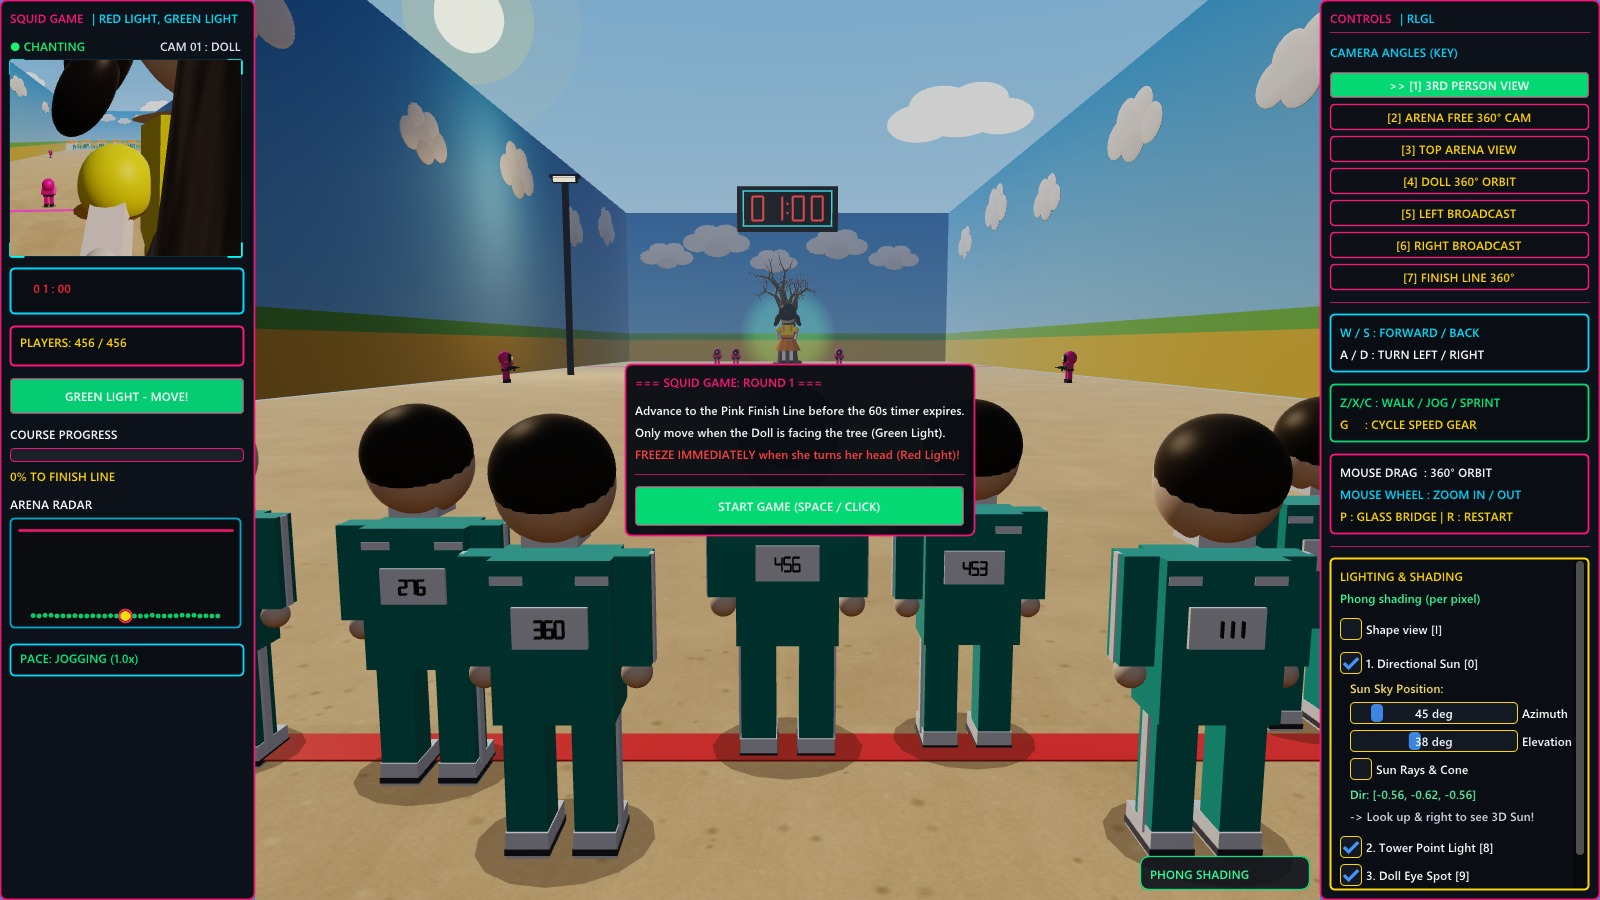
\includegraphics[width=\linewidth]{figures/ui_rlgl_start.jpg}
\caption{Start screen. Left panel: live doll camera, timer, player count, progress bar and a mini radar.
Right panel: camera buttons, controls and the lighting panel.}
\end{figure}

\begin{figure}[H]
\centering
\begin{subfigure}{0.495\linewidth}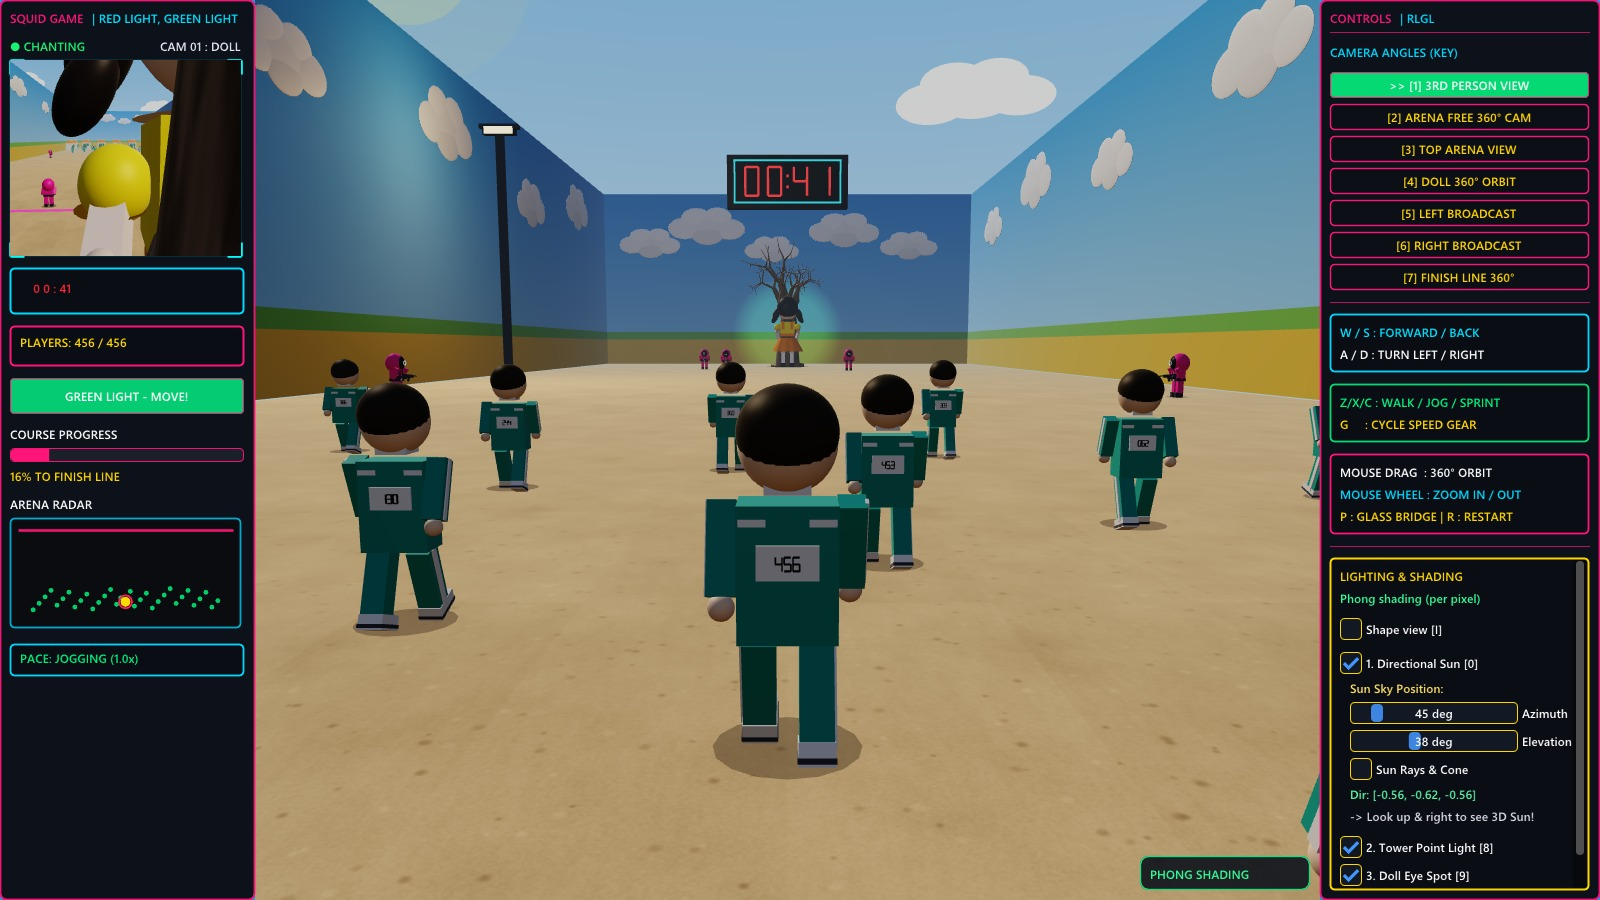
\includegraphics[width=\linewidth]{figures/ui_rlgl_green.jpg}
\caption{Green light -- everyone walks.}\end{subfigure}\hfill
\begin{subfigure}{0.495\linewidth}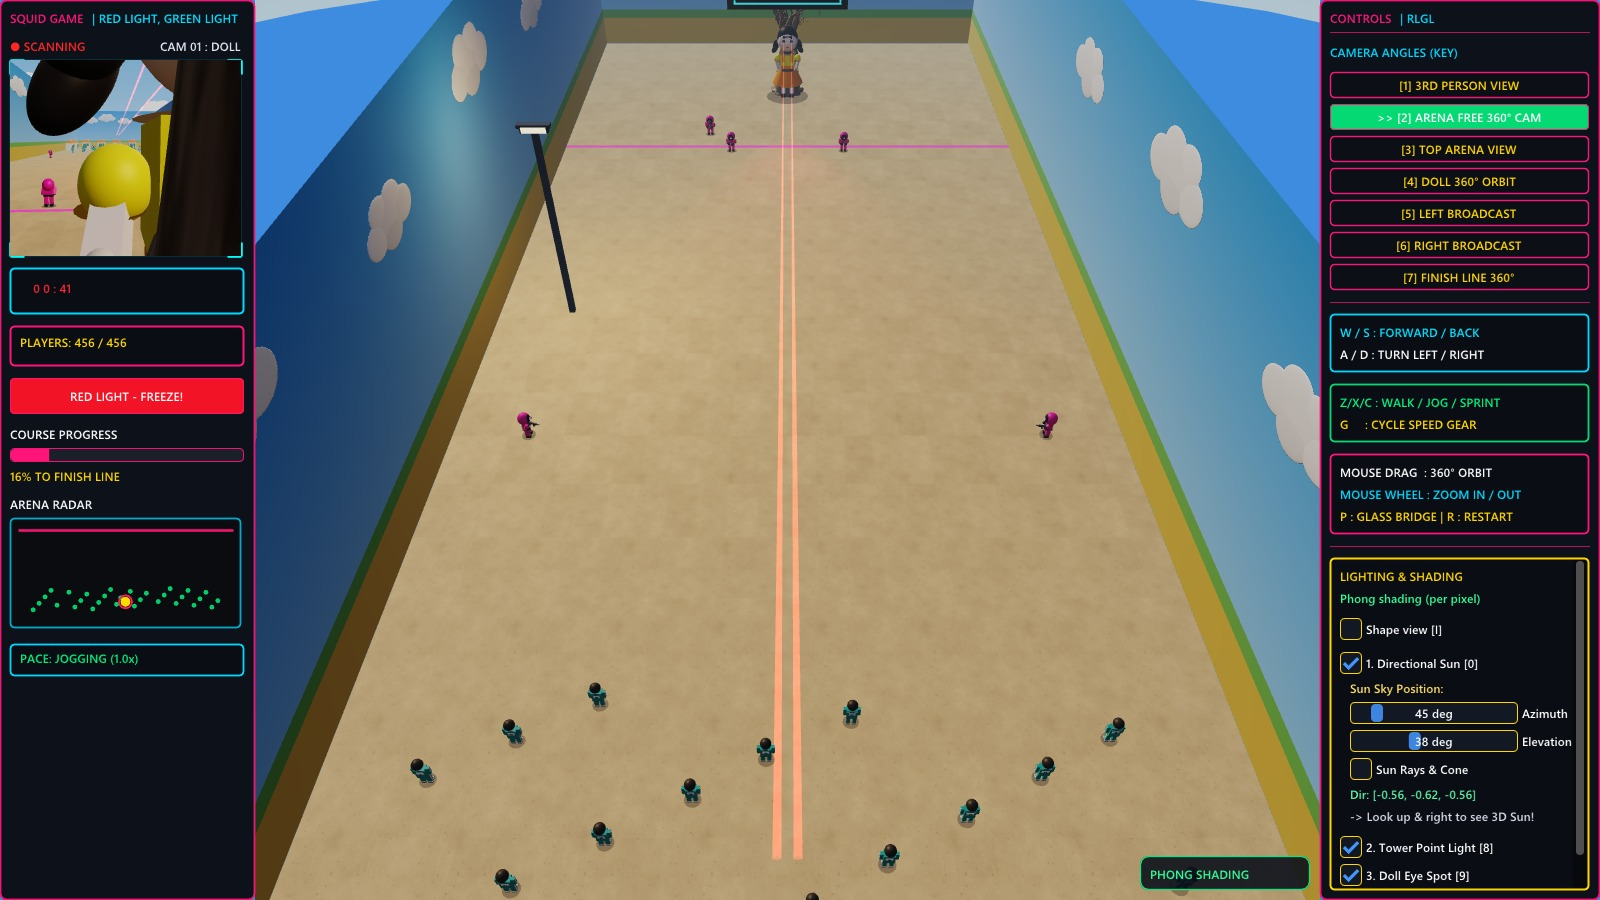
\includegraphics[width=\linewidth]{figures/ui_rlgl_red.jpg}
\caption{Red light -- the doll turns and scans with red lasers.}\end{subfigure}\\[4pt]
\begin{subfigure}{0.495\linewidth}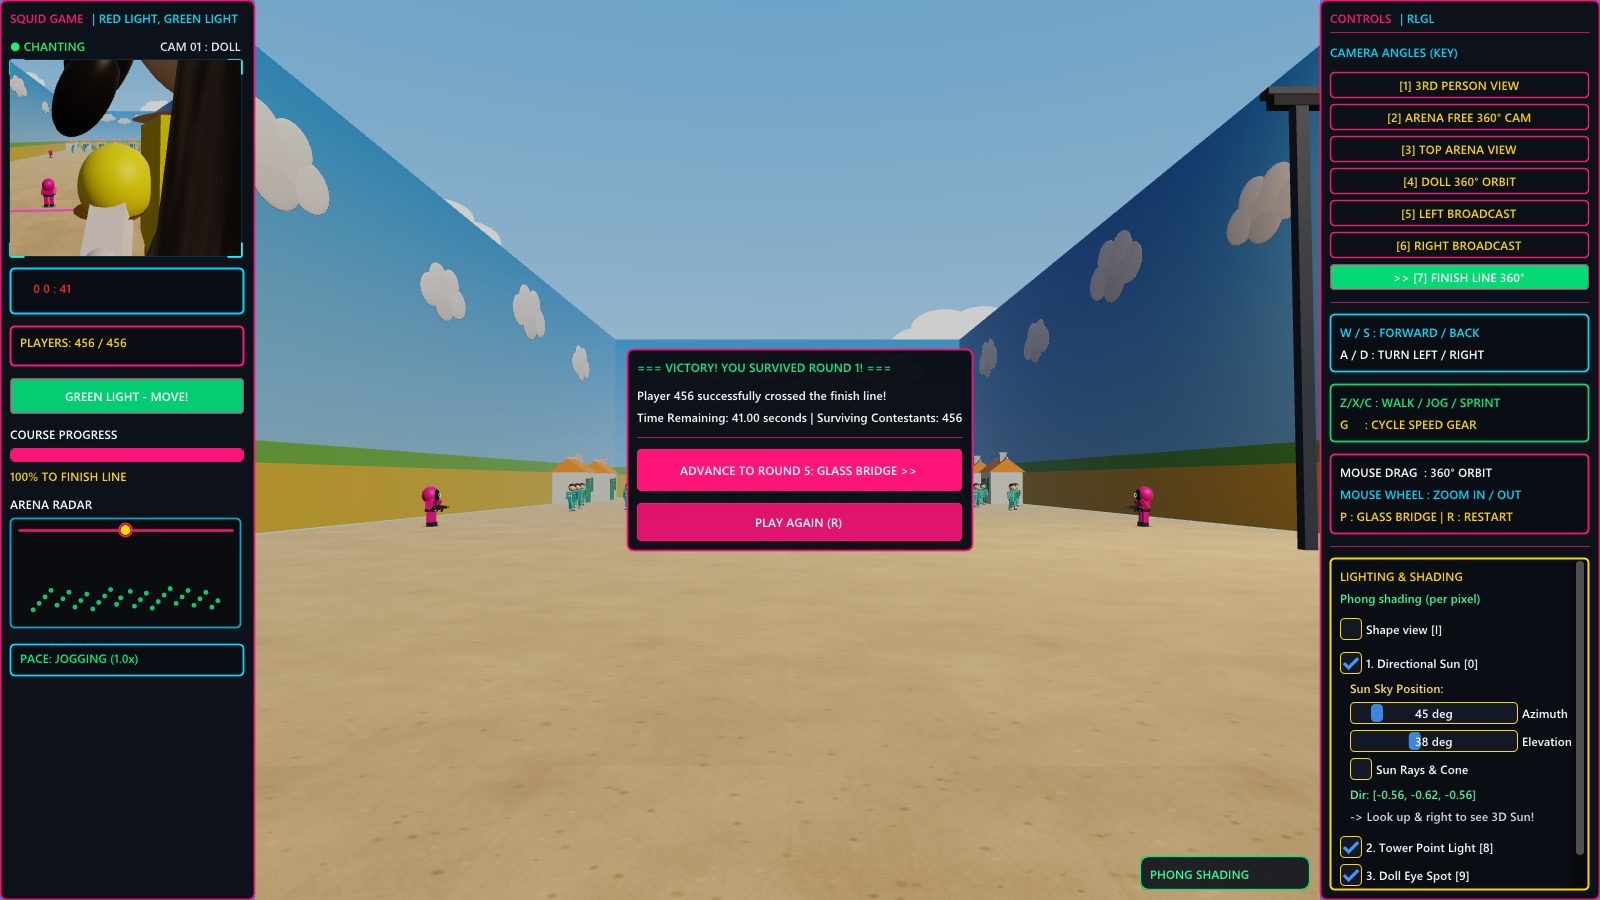
\includegraphics[width=\linewidth]{figures/ui_rlgl_won.jpg}
\caption{Player 456 crossed the finish line.}\end{subfigure}\hfill
\begin{subfigure}{0.495\linewidth}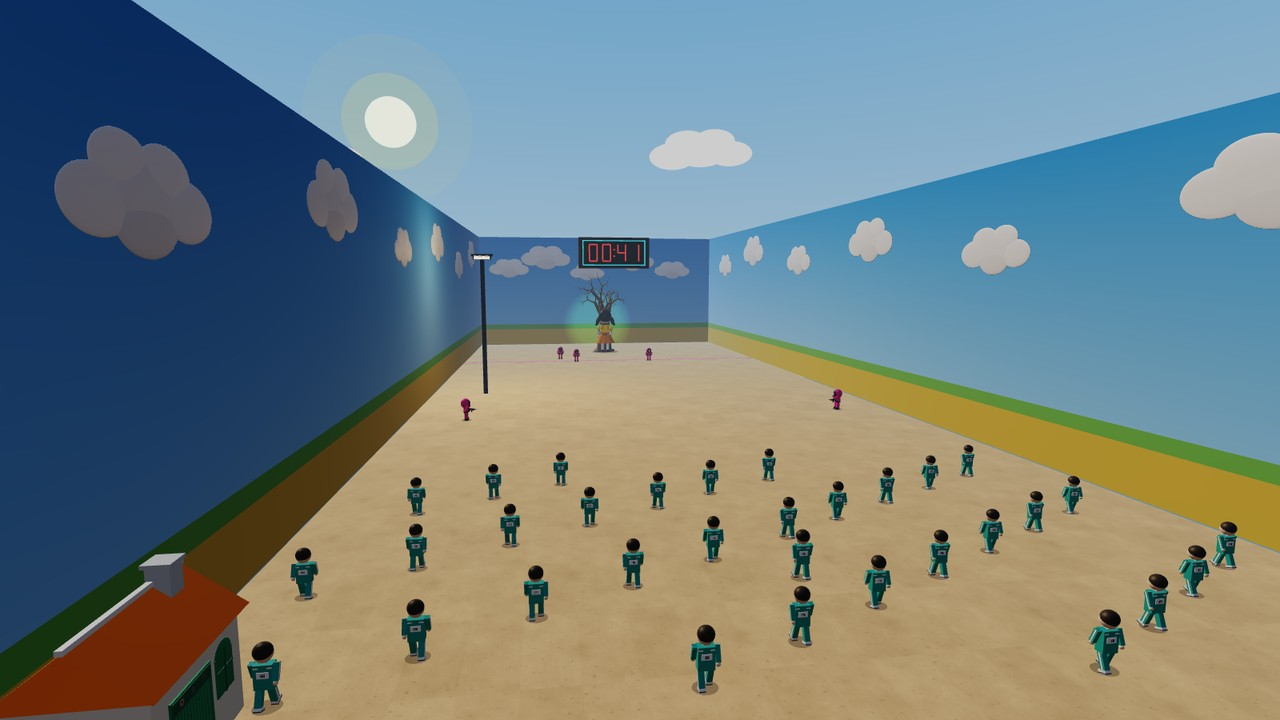
\includegraphics[width=\linewidth]{figures/rlgl_wide.jpg}
\caption{The whole arena, seen from behind the start.}\end{subfigure}
\caption{Round 1 while playing.}
\end{figure}

\subsection{Round 2: The Glass Bridge}

\begin{figure}[H]
\centering
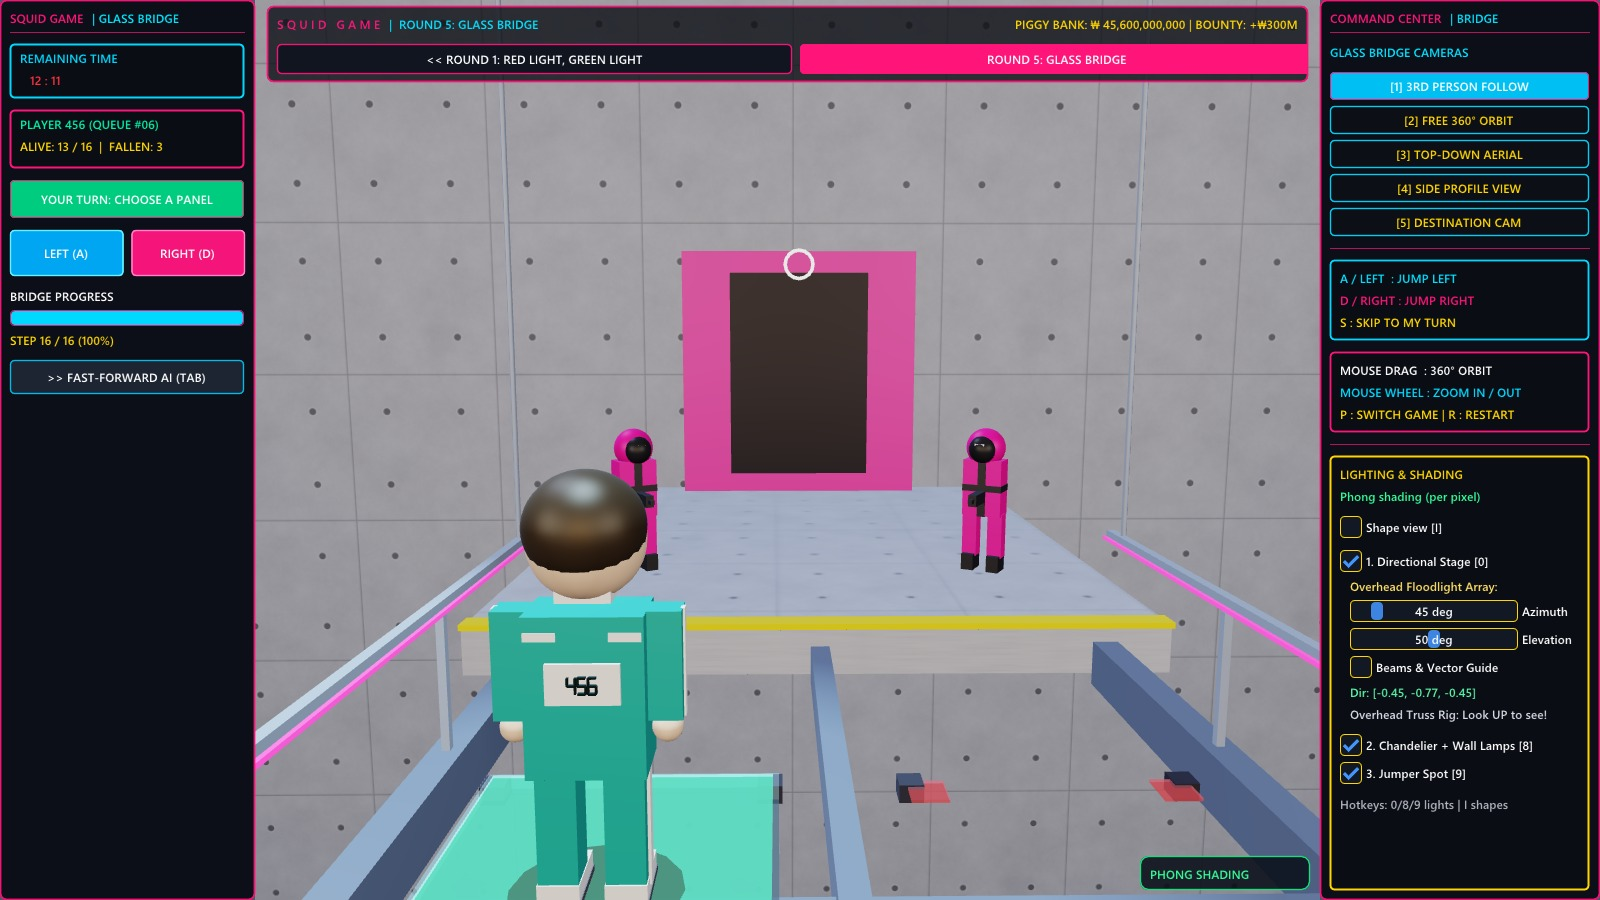
\includegraphics[width=0.74\linewidth]{figures/ui_gb_turn.jpg}
\caption{Player 456's turn. Green panes are proven safe, the red marks show broken panes. The cyan and pink
panes in front are the two choices: press \keybox{A} for left or \keybox{D} for right.}
\end{figure}

\begin{figure}[H]
\centering
\begin{subfigure}{0.32\linewidth}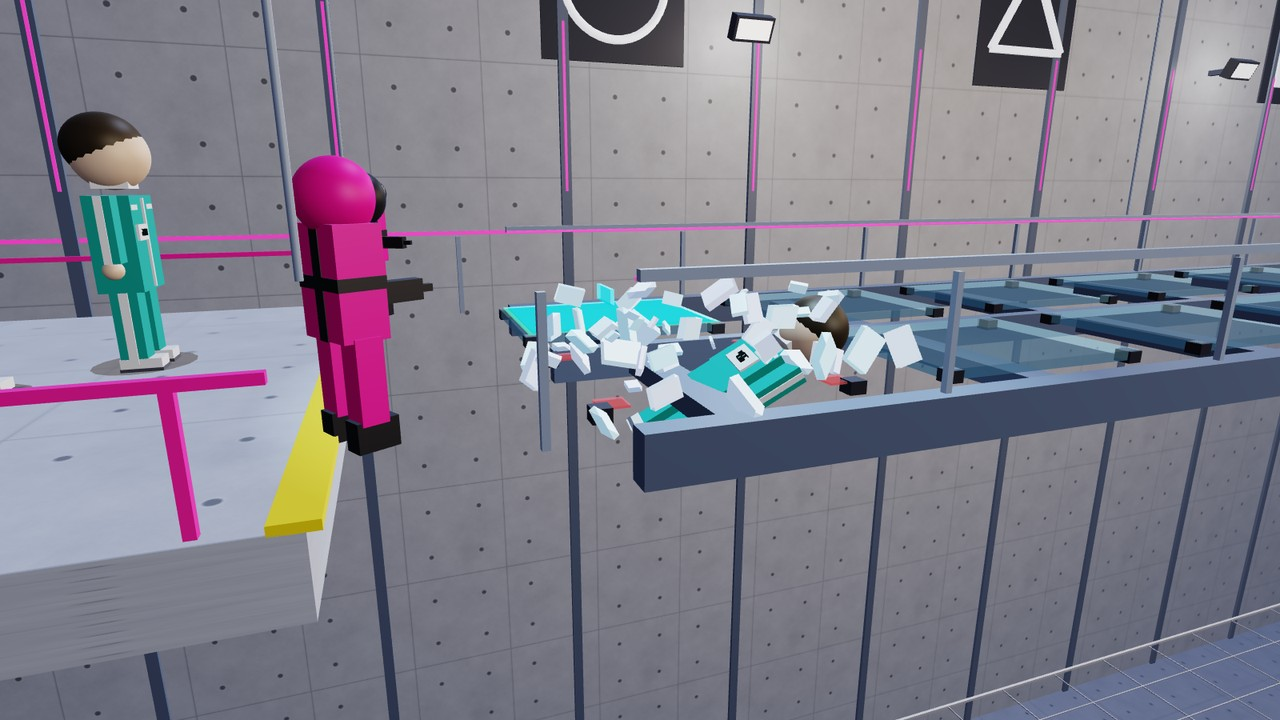
\includegraphics[width=\linewidth]{figures/gb_shatter.jpg}
\caption{Pane shatter physics}\end{subfigure}\hfill
\begin{subfigure}{0.32\linewidth}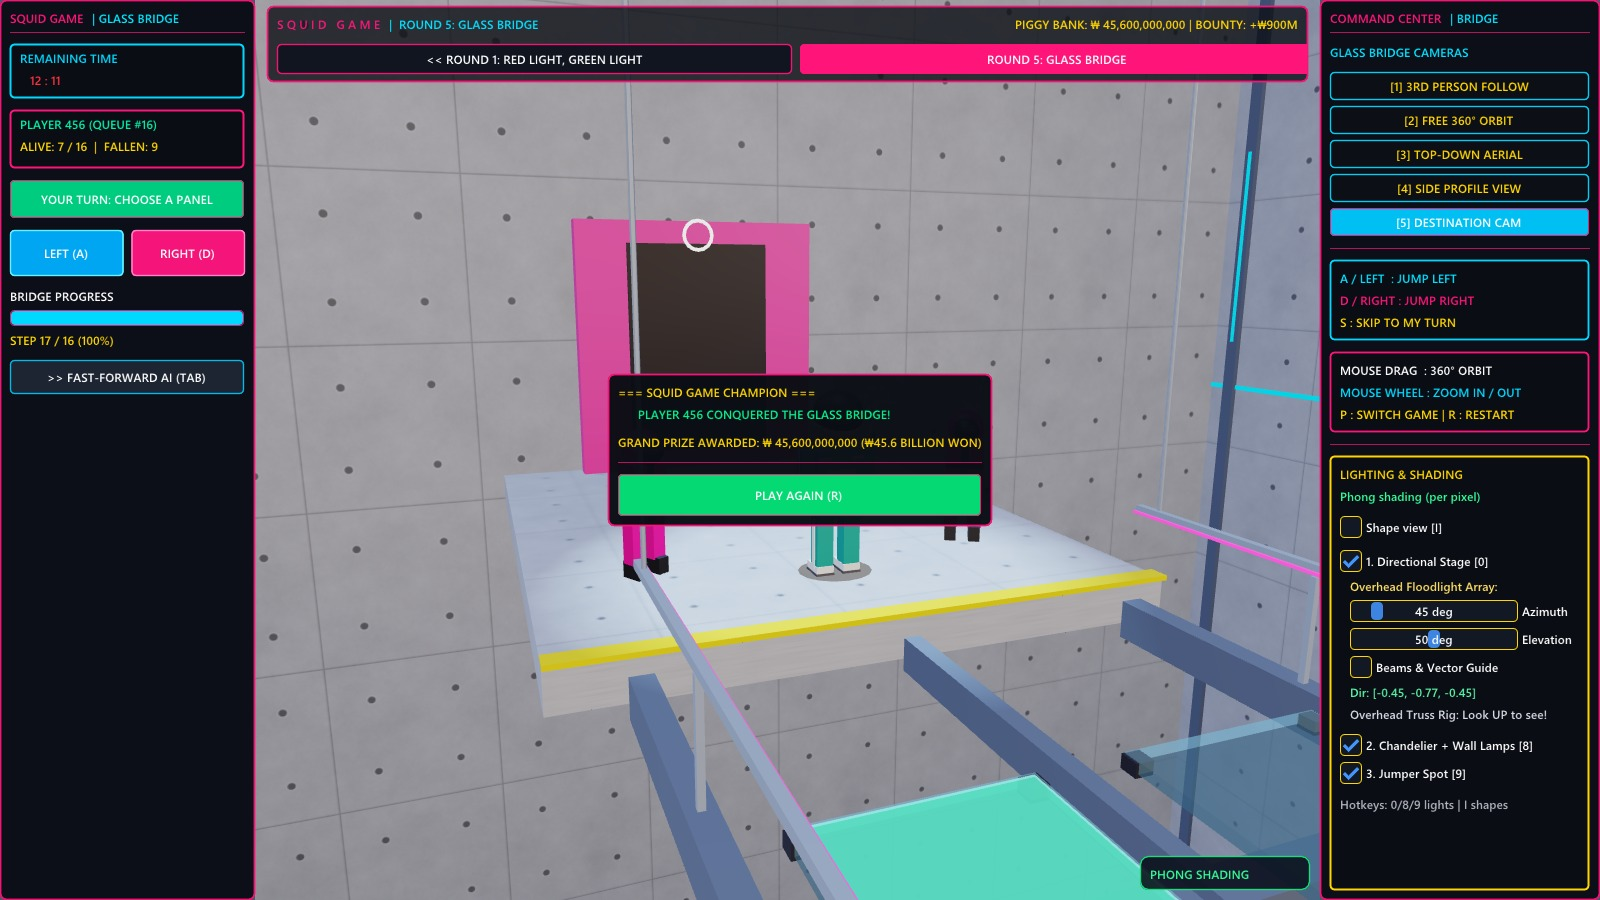
\includegraphics[width=\linewidth]{figures/ui_gb_won.jpg}
\caption{Player 456 victory}\end{subfigure}\hfill
\begin{subfigure}{0.32\linewidth}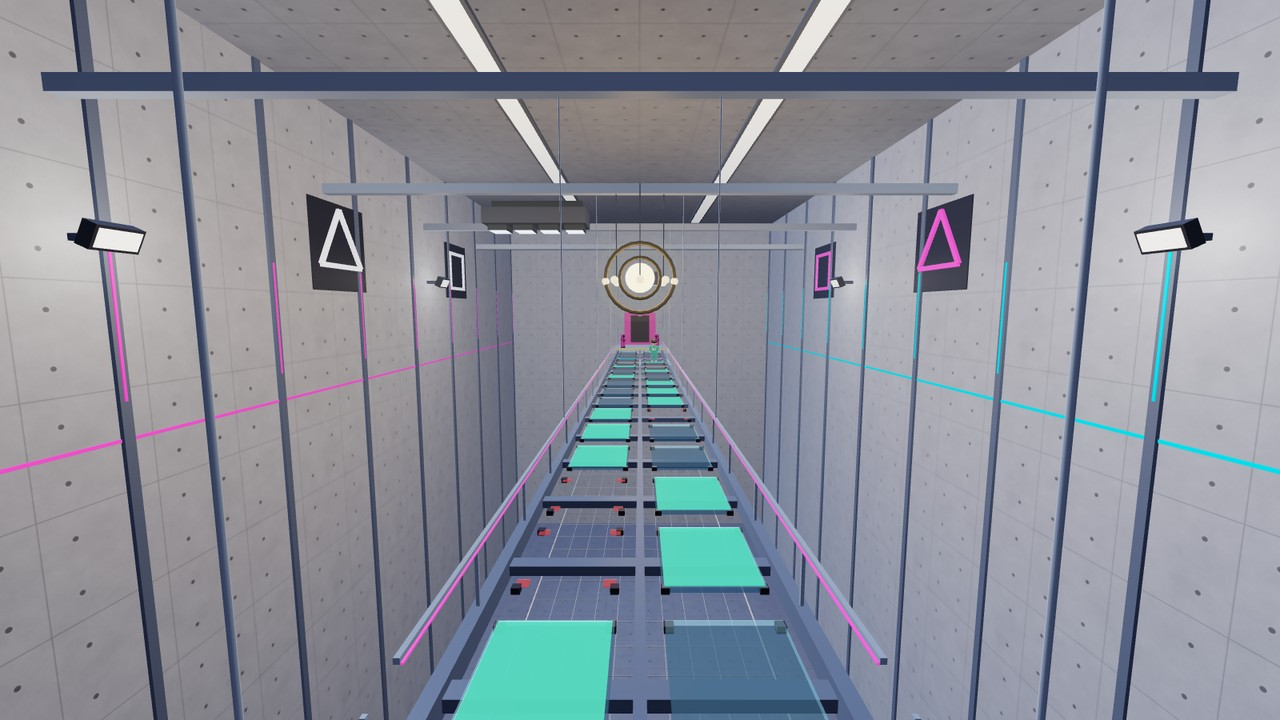
\includegraphics[width=\linewidth]{figures/gb_sides.jpg}
\caption{Light hall architecture}\end{subfigure}
\caption{Round 2 in-game moments and environment.}
\end{figure}

% =====================================================================================
\section{Tools Used}
% =====================================================================================
\begin{table}[H]
\centering\small
\rowcolors{2}{white}{rowgray}
\begin{tabularx}{\linewidth}{>{\bfseries}p{3.6cm} L}
\toprule
\rowcolor{white}Item & What we used \\ \midrule
Language & C++17, compiled with MinGW-w64 g++ \\
Graphics & OpenGL 3.3 Core Profile with GLSL 330 shaders \\
Window and input & GLFW 3 \\
OpenGL loader & GLAD \\
Math & GLM (vectors and matrices) \\
User interface & Dear ImGui (side panels, buttons, overlays) \\
Images & stb\_image (loads the PNG textures) \\
Sound & Windows multimedia API (song + generated sound effects) \\
3D models & None imported -- every object is built in code from basic shapes \\
\bottomrule
\end{tabularx}
\end{table}

% =====================================================================================
\section{How to Play}
% =====================================================================================
\begin{table}[H]
\centering\small
\rowcolors{2}{white}{rowgray}
\begin{tabularx}{\linewidth}{>{\ttfamily}p{3.4cm} L}
\toprule
\rowcolor{white}\normalfont\textbf{Key} & \textbf{Action} \\ \midrule
\multicolumn{2}{l}{\cellcolor{white}\textbf{\color{sgteal}Both rounds}} \\
P & Switch between Round 1 and Round 2 \\
R & Restart the round \\
0 / 8 / 9 & Turn the directional / point / spot light on or off \\
I & Shape view: color every part by its basic shape \\
Mouse drag, wheel & Orbit the camera, zoom \\
\multicolumn{2}{l}{\cellcolor{white}\textbf{\color{sgteal}Round 1}} \\
W / S & Walk forward / backward \\
A / D, Q / E & Turn left / right, step sideways \\
Z / X / C (or Shift) & Walk / jog / sprint \\
1 -- 7 & Camera modes \\
\multicolumn{2}{l}{\cellcolor{white}\textbf{\color{sgteal}Round 2}} \\
A / D & Jump to the left / right pane \\
S & Skip to Player 456's turn \\
Tab & Fast-forward the other players \\
1 -- 5 & Camera modes \\
7 & Toggle wall lamps \\
\bottomrule
\end{tabularx}
\end{table}

% =====================================================================================
\section{Program Structure}
% =====================================================================================
The code is split into small folders, one job each:

\begin{table}[H]
\centering\small
\rowcolors{2}{white}{rowgray}
\begin{tabularx}{\linewidth}{>{\ttfamily}p{3.5cm} L}
\toprule
\rowcolor{white}\normalfont\textbf{Folder} & \textbf{What it does} \\ \midrule
main\_modern.cpp & Main loop, keyboard/mouse, lights setup, user interface, capture mode \\
engine/ & OpenGL building blocks: Shader, VAO, VBO, EBO, Mesh, Texture, basic shapes, matrix stack \\
shaders/ & \texttt{default.vert} and \texttt{default.frag} (Phong lighting) \\
render/ & Light fixture models, the three textures \\
contestants/, guards/, doll/ & The characters \\
environment/ & Round 1 arena: sky, sand, walls, houses, clock \\
glassbridge/ & Round 2: bridge, hall, platforms, glass shards, cameras, game rules \\
camera/, audio/ & Round 1 cameras, sound \\
core/Config.h & All colors, sizes, speeds and timers in one place \\
tools/ & Shape showcase (report figures), texture generator, figure script \\
\bottomrule
\end{tabularx}
\end{table}

Every frame the program does the same five steps:

\begin{figure}[H]
\centering
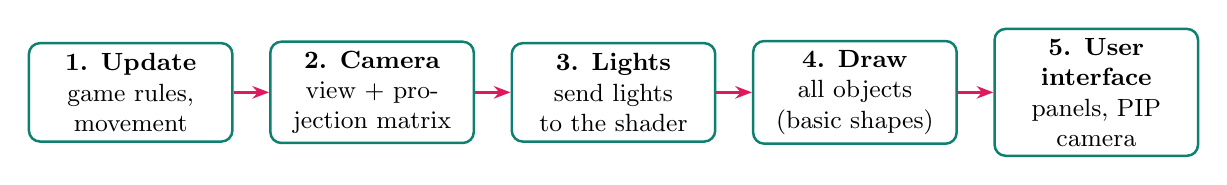
\begin{tikzpicture}[
  node distance=0.45cm,
  box/.style={draw=sgteal, line width=0.9pt, rounded corners=4pt, fill=white, align=center,
              minimum height=1.25cm, text width=2.35cm, font=\small},
  arr/.style={-{Stealth[length=6pt]}, line width=1pt, color=sgpink}]
\node[box] (a) {\textbf{1. Update}\\game rules, movement};
\node[box, right=of a] (b) {\textbf{2. Camera}\\view + projection matrix};
\node[box, right=of b] (c) {\textbf{3. Lights}\\send lights to the shader};
\node[box, right=of c] (d) {\textbf{4. Draw}\\all objects (basic shapes)};
\node[box, right=of d] (e) {\textbf{5. User interface}\\panels, PIP camera};
\draw[arr] (a) -- (b); \draw[arr] (b) -- (c); \draw[arr] (c) -- (d); \draw[arr] (d) -- (e);
\end{tikzpicture}
\caption{What happens in one frame (about 60 times per second).}
\end{figure}

\textbf{World size.} All sizes are in game units. Round 1 arena: $x$ from $-24$ to $24$, $z$ from $-75$ to $75$,
walls 22 high. Start line at $z=-52$, finish line at $z=45$, doll at $(0,0,58)$, 2.6 times bigger than normal.
Round 2: 16 glass steps, the first at $z=3$, one step every 3.3 units, at height $y=16$.

% =====================================================================================
\section{Basic Shapes}\label{sec:shapes}
% =====================================================================================
The whole game is built from only seven basic shapes. Figure~\ref{fig:shapes} shows each one, rendered by the
program itself. The thin dark lines show the triangles the GPU actually draws.

\begin{figure}[H]
\centering
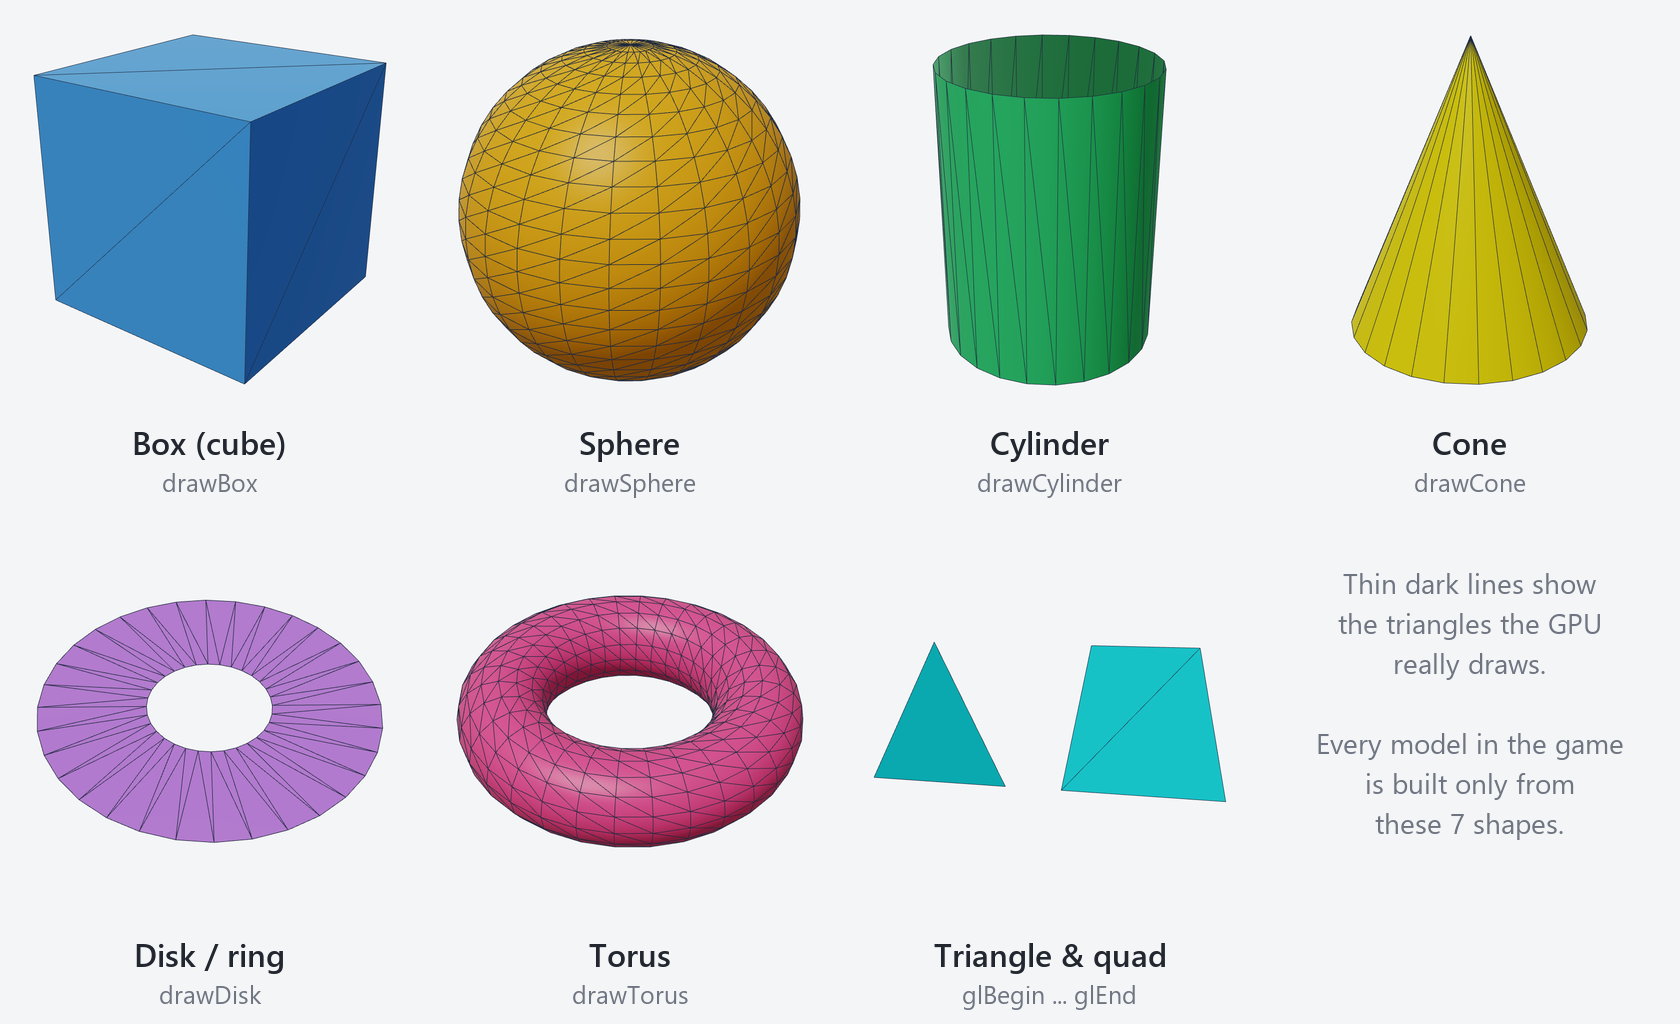
\includegraphics[width=0.92\linewidth]{figures/basic_shapes.png}
\caption{The seven basic shapes and the function that draws each one.}
\label{fig:shapes}
\end{figure}

\begin{table}[H]
\centering\small
\rowcolors{2}{white}{rowgray}
\begin{tabularx}{\linewidth}{p{2.4cm} p{3.6cm} L L}
\toprule
\rowcolor{white}\textbf{Shape} & \textbf{Settings} & \textbf{How it is made} & \textbf{Used for (examples)} \\ \midrule
\shBox & width, height, depth & 6 faces $\times$ 4 corners = 24 vertices, 12 triangles & bodies, legs, walls, glass panes, rails \\
\shSph & radius & 24 rings $\times$ 24 slices = 1152 triangles & heads, eyes, hands, clouds, bulbs \\
\shCyl & bottom radius, top radius, height & a ring of side rectangles (no lids) & tree branches, neck, cables \\
\shCon & radius, height & a cylinder whose top radius is 0 & (cone beams) \\
\shDsk & inner radius, outer radius & flat ring of triangles & doll's collar, lens, sleeve cuffs \\
\shTor & tube radius, ring radius & a tube bent into a ring & chandelier rings, circle symbols \\
\shPol & any corner points & triangles / quads typed in by hand & roofs, sand floor, skirt, sky \\
\bottomrule
\end{tabularx}
\caption{The basic shapes. A box is always made as a $1\times1\times1$ cube and stretched with \emph{scale};
a sphere is always radius 1 and scaled to the wanted size.}
\end{table}

% =====================================================================================
\clearpage
\section{Transformations}\label{sec:transform}
% =====================================================================================
Each shape is moved into place with three transformations. In 3D we use $4\times4$ matrices:

\[
T=\begin{bmatrix}1&0&0&t_x\\0&1&0&t_y\\0&0&1&t_z\\0&0&0&1\end{bmatrix}\quad
S=\begin{bmatrix}s_x&0&0&0\\0&s_y&0&0\\0&0&s_z&0\\0&0&0&1\end{bmatrix}\quad
R_y(\theta)=\begin{bmatrix}\cos\theta&0&\sin\theta&0\\0&1&0&0\\-\sin\theta&0&\cos\theta&0\\0&0&0&1\end{bmatrix}
\]

\begin{itemize}
  \item \textbf{Translate} ($T$ / \texttt{glTranslatef}) moves a part or character in 3D world or local coordinate space.
  \item \textbf{Rotate} ($R$ / \texttt{glRotatef}) turns a part or body joint (e.g., pendulum limb swing, doll head $180^\circ$ scan).
  \item \textbf{Scale} ($S$ / \texttt{glScalef}) sizes primitives: deforms unit boxes and spheres into anatomical body parts (thin soles, flat walls, oval blushes) and scales the colossal doll ($2.5\times$) relative to normal contestants.
  \item \textbf{Hierarchical Modeling} (\texttt{glPushMatrix} / \texttt{glPopMatrix}): A part's final matrix is $\text{parent} \times T \times R \times S$. Child parts inherit parent transformations (the hand follows the arm, and the arm follows the body). \texttt{glPushMatrix()} preserves the parent matrix and \texttt{glPopMatrix()} restores it, isolating local changes from adjacent objects.
\end{itemize}

Example -- one leg of Player 456 (from \texttt{Contestants.cpp}):
\begin{lstlisting}
glPushMatrix();
glTranslatef(side * 0.15f, 0.62f, 0.0f);  // move to the hip joint
glRotatef(legAngle, 1.0f, 0.0f, 0.0f);     // swing the leg forward/back (walk)
glTranslatef(0.0f, -0.279f, 0.0f);         // the leg hangs below the hip
glScalef(0.18f, 0.558f, 0.18f);            // stretch the unit cube into a leg
glutSolidCube(1.0);
glPopMatrix();
\end{lstlisting}
\note{Note: these old-style function names are kept on purpose, but they run on modern OpenGL. Our
\texttt{GLCompat} layer keeps its own matrix stack (GLM) and draws the shape with VAO/VBO buffers and shaders.}

\subsection{Multi-View Orthographic and Isometric Projections}
In engineering computer graphics and 3D geometric modeling, standard multi-view projections are employed to inspect and verify 3D objects across principal coordinate axes without perspective distortion:
\begin{itemize}
  \item \textbf{Front View (Elevation):} Projection along the principal viewing axis ($xy$-plane) displaying the frontal silhouette, facial features, and vertical proportion hierarchy.
  \item \textbf{Side View (Profile):} Projection along the orthogonal lateral axis ($yz$-plane) capturing depth profile, limb swing stance, and front-to-back extents.
  \item \textbf{Top View (Plan):} Projection down the vertical $y$-axis ($xz$-plane) displaying structural footprint, horizontal symmetry, and planar orientations.
  \item \textbf{Isometric View:} An axonometric 3D projection where coordinate axes are equally foreshortened, revealing volumetric depth and spatial relationships ($R_x\,35.264^\circ \cdot R_y\,45^\circ$).
\end{itemize}

\[
P_{\text{ortho}} = \begin{bmatrix}
\frac{1}{r} & 0 & 0 & 0 \\
0 & \frac{1}{t} & 0 & 0 \\
0 & 0 & -\frac{2}{f-n} & -\frac{f+n}{f-n} \\
0 & 0 & 0 & 1
\end{bmatrix}
\qquad
R_{\text{iso}} = R_x(35.264^\circ) \cdot R_y(45^\circ)
\]
Canonical views are rendered with \texttt{glm::ortho(-w, w, -h, h, 0.1f, 100.0f)} and \texttt{glm::lookAt(eye, center, up)}.

% =====================================================================================
\clearpage
\section{Objects and the Shapes They Are Made Of}\label{sec:objects}
% =====================================================================================
Every 3D model in the project is procedurally assembled from the seven primitive shapes introduced in Section~\ref{sec:shapes}, without importing third-party mesh files. For each object, we provide a complete technical specification sheet across three core dimensions:
\begin{enumerate}
  \item \textbf{Canonical Multi-View Projections:} High-resolution orthogonal elevations and axonometric view displaying \textbf{(a) Front (elevation)}, \textbf{(b) Side (profile)}, \textbf{(c) Top (plan)}, and \textbf{(d) Isometric} aspects.
  \item \textbf{Hierarchical Shape Decomposition:} The finished textured model rendered alongside its exploded primitive view, color-coded by shape category:
  \shape{cbox}{Box}\quad \shape{csphere}{Sphere}\quad \shape{ccyl}{Cylinder}\quad \shape{ccone}{Cone}\quad
  \shape{cdisk}{Disk}\quad \shape{ctorus}{Torus}\quad \shape{cpoly}{Polygon}.
  \item \textbf{Mathematical Transformation Hierarchy:} Exact local translations ($T$), rotations ($R$), scales ($S$), and primitive dimensions.
\end{enumerate}

\textbf{Coordinate Conventions and Hierarchy.} All local coordinate descriptions use a right-handed Cartesian system: $+x$ points right, $+y$ points vertically upward, and $+z$ points forward along the principal facing direction. Child parts inherit their parent's coordinate frame via the matrix stack (\texttt{glPushMatrix()} / \texttt{glPopMatrix()}). The notation ``$\pm$'' designates symmetric left/right pairs. Rotations indicate axis and angle (e.g., $R_x\,25^\circ$).

\begin{table}[H]
\centering\small
\rowcolors{2}{white}{rowgray}
\begin{tabularx}{\linewidth}{p{2.8cm} p{2.2cm} L}
\toprule
\rowcolor{white}\textbf{Shape Primitive} & \textbf{Color Code} & \textbf{Parametric Generation / Topology} \\ \midrule
\shBox & Cyan & 12 triangles from unit cube, scaled by $(s_x, s_y, s_z)$ \\
\shSph & Orange & UV sphere ($24\times24$ rings), polar coordinates $(\theta, \phi)$ \\
\shCyl & Blue & Longitudinal triangle strip with taper $(r_{\text{base}} \to r_{\text{top}})$ \\
\shCon & Green & Degenerate tapered cylinder ($r_{\text{top}} = 0$, apex vertex) \\
\shDsk & Yellow & Planar annular ring ($r_{\text{inner}} \le r \le r_{\text{outer}}$) \\
\shTor & Magenta & Torus swept by ring radius $R$ and tube radius $r$ \\
\shPol & Red & Planar vertex arrays (roofs, sand ground, sky quads) \\
\bottomrule
\end{tabularx}
\caption{Primitive shapes and color assignments used in all exploded decomposition figures.}
\end{table}

\begin{table}[H]
\centering\small
\rowcolors{2}{white}{rowgray}
\begin{tabularx}{\linewidth}{L r r r r r r r r}
\toprule
\rowcolor{white}\textbf{Object} & \textbf{Box} & \textbf{Sphere} & \textbf{Cyl.} & \textbf{Disk} & \textbf{Torus} & \textbf{Poly.} & \textbf{Line} & \textbf{Total} \\ \midrule
Player 456 / contestant & 49 & 4 & & & & & & 53 \\
Pink guard (Round 1) & 19 & 4 & & & & & & 23 \\
Bridge guard (Round 2) & 9 & 2 & & & 1 & & & 12 \\
Young-hee doll (body) & 40 & 30 & 3 & 5 & & 18 & & 96 \\
Young-hee doll head & 10 & 40 & 1 & & & & & 51 \\
Dead tree & & 157 & 156 & & & & & 313 \\
Village house & 21 & 1 & & & 3 & 2 & 2 & 29 \\
Countdown clock & 55 & & & & & & & 55 \\
Glass bridge (3 steps shown) & 48 & & & & & & & 48 \\
Start platform & 17 & & & & & & & 17 \\
Light fixtures (5 kinds) & 21 & 9 & 1 & 1 & 2 & & & 34 \\
\bottomrule
\end{tabularx}
\caption{Number of parts in each object, counted by the program while drawing it.}
\end{table}

\textbf{Documentation Structure.} The following sheets detail each 3D asset individually on a dedicated page, verifying its geometric symmetry, proportions, and procedural transformation pipeline.

% -------------------------------------------------------------------------------------
\clearpage
\subsection{Player 456 and the other contestants}
% -------------------------------------------------------------------------------------
The same model is used for every contestant in both rounds; only the number on the chest and back changes.
\textbf{Placed in the world with:} $T(x,0,z)\cdot R_y(\text{facing})\cdot S(1.15)$ (other contestants $S(1.10)$).

\begin{figure}[H]
\centering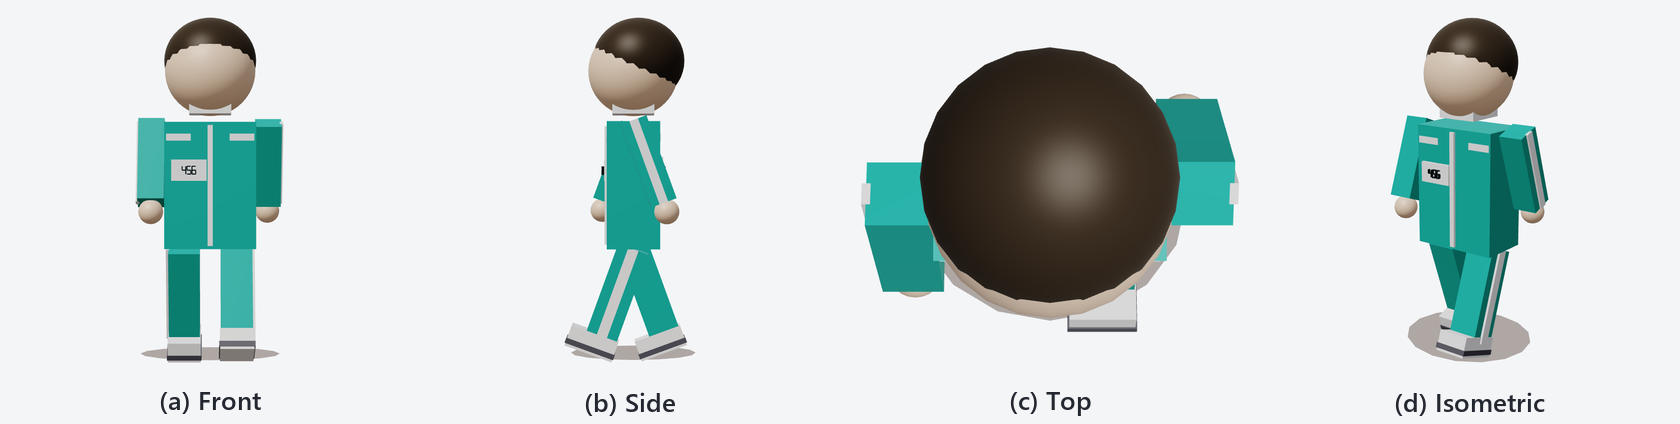
\includegraphics[width=0.84\linewidth]{figures/views_player.png}
\caption{Player 456 multi-view projections: (a) Front, (b) Side profile, (c) Top view, (d) Isometric 3D view.}
\end{figure}

\begin{figure}[H]
\centering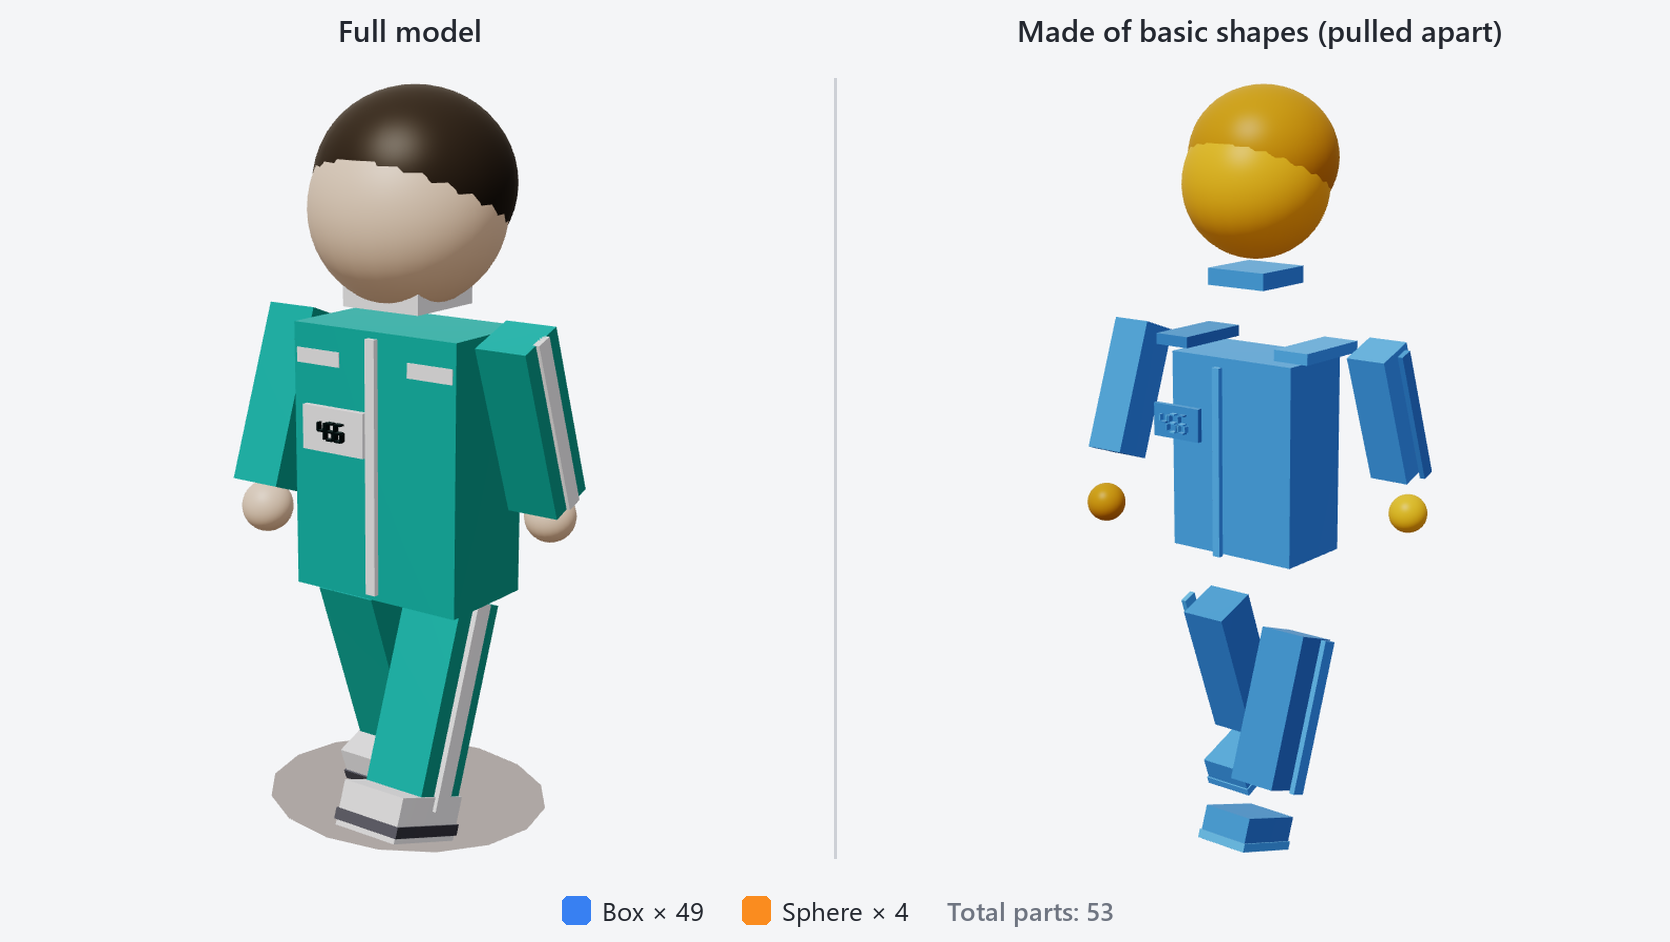
\includegraphics[width=0.50\linewidth]{figures/decomp_player.png}
\caption{Player 456 shape decomposition: 49 boxes and 4 spheres.}
\end{figure}

\begin{parttable}
Legs $\times2$ & \shBox & $0.18\times0.56\times0.18$ & $(\pm0.15,\ 0.34,\ 0)$ & $R_x$ swing at hip ($y{=}0.62$) \\
Leg stripes $\times2$ & \shBox & $0.02\times0.56\times0.06$ & $(\pm0.245,\ 0.34,\ 0)$ & moves with leg \\
Shoes $\times2$ & \shBox & $0.19\times0.12\times0.28$ & $(\pm0.15,\ 0.04,\ 0.04)$ & moves with leg \\
Shoe soles $\times2$ & \shBox & $0.20\times0.03\times0.29$ & $(\pm0.15,\ 0.01,\ 0.04)$ & moves with leg \\
Jacket (body) & \shBox & $0.52\times0.72\times0.30$ & $(0,\ 0.98,\ 0)$ & -- \\
Zipper & \shBox & $0.03\times0.68\times0.02$ & $(0,\ 0.98,\ 0.16)$ & -- \\
Shoulder stripes $\times2$ & \shBox & $0.14\times0.04\times0.31$ & $(\pm0.18,\ 1.25,\ 0)$ & -- \\
Chest number patch & \shBox & $0.20\times0.12\times0.02$ & $(-0.12,\ 1.07,\ 0.16)$ & -- \\
Back number patch & \shBox & $0.32\times0.18\times0.02$ & $(0,\ 1.05,\ -0.16)$ & $R_y\,180^\circ$ \\
Number ``456'' (front + back) & \shBox{} $\times30$ & 7-segment bars, $0.021\times0.005$ (front) & on the patches & -- \\
Arms $\times2$ & \shBox & $0.15\times0.49\times0.15$ & $(\pm0.335,\ 1.10,\ 0)$ & $R_x$ swing at shoulder ($y{=}1.34$) \\
Arm stripes $\times2$ & \shBox & $0.02\times0.49\times0.05$ & $(\pm0.41,\ 1.10,\ 0)$ & moves with arm \\
Hands $\times2$ & \shSph & radius $0.07$ & $(\pm0.335,\ 0.80,\ 0)$ & moves with arm \\
Collar & \shBox & $0.24\times0.06\times0.24$ & $(0,\ 1.42,\ 0)$ & -- \\
Face & \shSph & radius $0.26$ & $(0,\ 1.64,\ 0)$ & -- \\
Hair & \shSph & radius $0.26$, $S(1.02,0.95,1.02)$ & $(0,\ 1.70,\ -0.03)$ & -- \\
\end{parttable}

% -------------------------------------------------------------------------------------
\clearpage
\subsection{Pink guard (Round 1)}
% -------------------------------------------------------------------------------------
Five guards stand around the arena. The mask symbol shows the rank: circle, triangle or square.
\textbf{Placed with:} $T(x,0,z)\cdot R_y(\text{facing})\cdot S(1.2)$. When a guard shoots, it turns to the target:
$\text{facing}=\operatorname{atan2}(x_t-x_g,\ z_t-z_g)$.

\begin{figure}[H]
\centering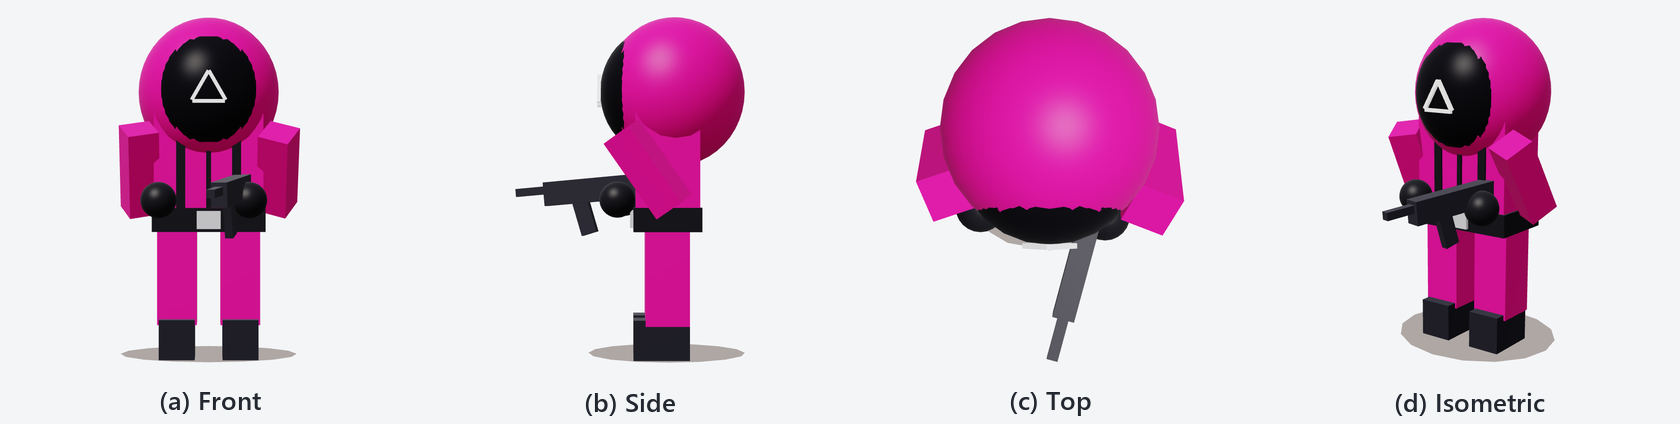
\includegraphics[width=0.84\linewidth]{figures/views_guard.png}
\caption{Pink guard multi-view projections: (a) Front, (b) Side profile, (c) Top view, (d) Isometric 3D view.}
\end{figure}

\begin{figure}[H]
\centering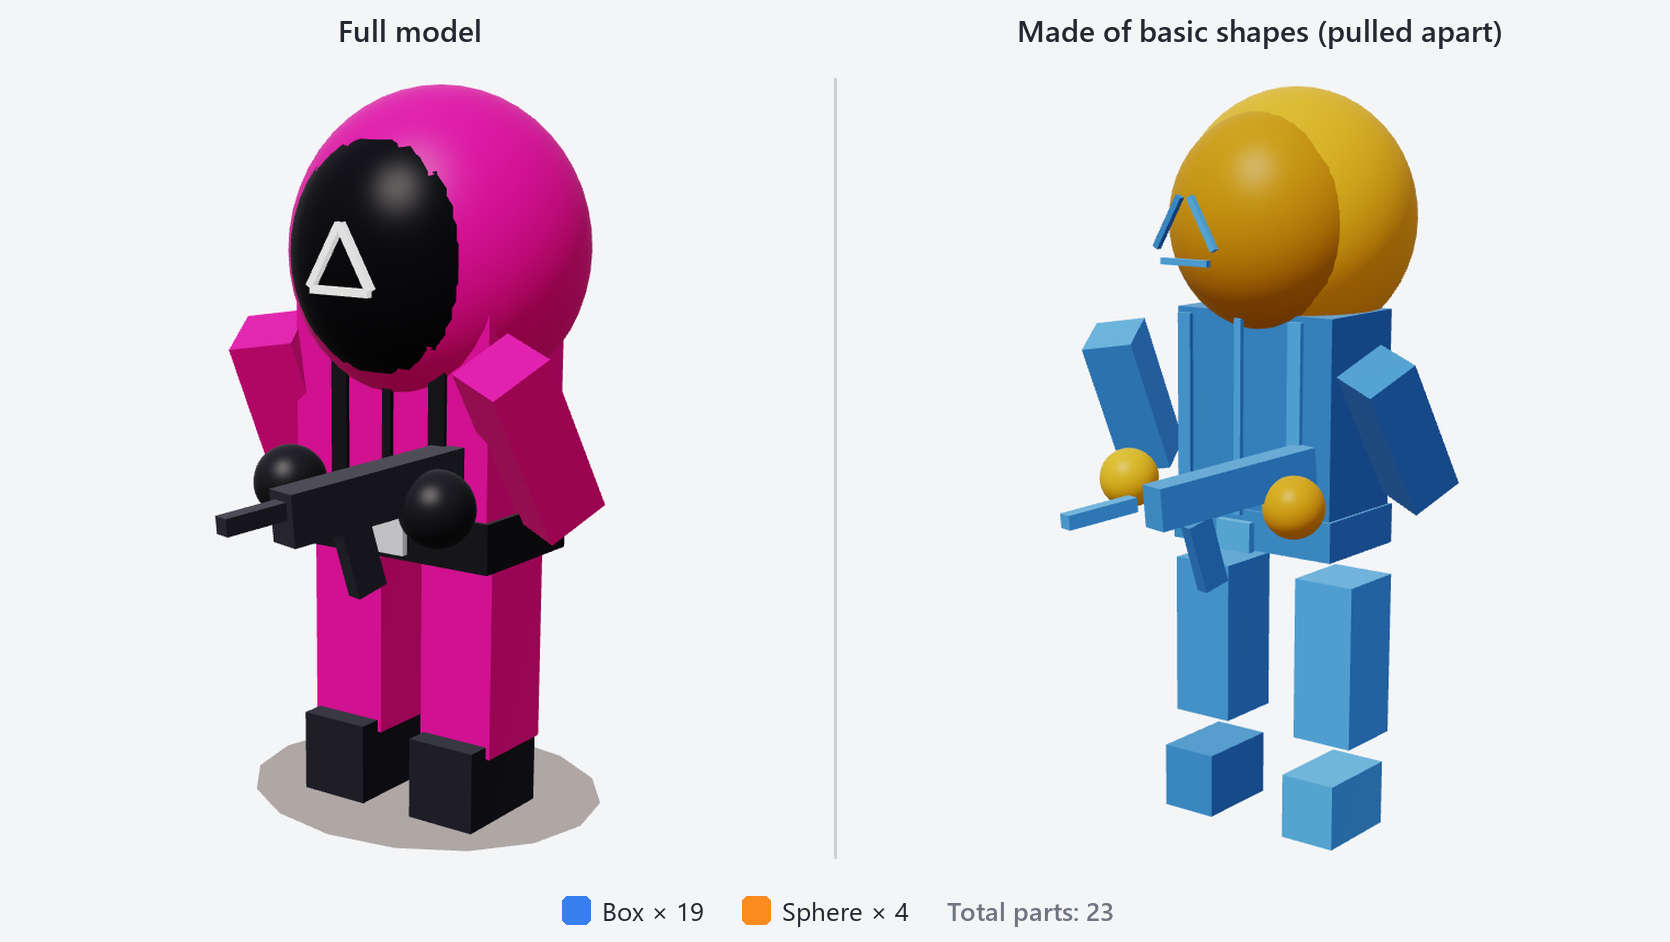
\includegraphics[width=0.50\linewidth]{figures/decomp_guard.png}
\caption{Triangle guard shape decomposition: 19 boxes and 4 spheres.}
\end{figure}

\begin{parttable}
Boots $\times2$ & \shBox & $0.18\times0.20\times0.28$ & $(\pm0.16,\ 0.10,\ 0.03)$ & -- \\
Legs $\times2$ & \shBox & $0.20\times0.50\times0.22$ & $(\pm0.16,\ 0.42,\ 0)$ & -- \\
Body & \shBox & $0.55\times0.60\times0.32$ & $(0,\ 0.95,\ 0)$ & -- \\
Zipper & \shBox & $0.024\times0.58\times0.015$ & $(0,\ 0.95,\ 0.165)$ & -- \\
Belt + buckle & \shBox{} $\times2$ & $0.57\times0.12\times0.34$; $0.12\times0.09\times0.025$ & $(0,\ 0.70,\ 0)$; $(0,\ 0.70,\ 0.175)$ & -- \\
Shoulder straps $\times2$ & \shBox & $0.045\times0.50\times0.015$ & $(\pm0.14,\ 0.98,\ 0.163)$ & -- \\
Neck collar & \shBox & $0.34\times0.09\times0.32$ & $(0,\ 1.22,\ 0)$ & -- \\
Left / right arm & \shBox & $0.16\times0.45\times0.16$ & $(-0.35,\ 0.95,\ 0.08)$ / $(0.35,\ 0.95,\ 0.10)$ & $R_x25^\circ R_y20^\circ$ / $R_x35^\circ R_y{-25}^\circ$ \\
Gloves $\times2$ & \shSph & radius $0.09$ & $(-0.25,\ 0.80,\ 0.22)$, $(0.20,\ 0.80,\ 0.25)$ & -- \\
Hood & \shSph & $S(0.36,0.38,0.36)$ & $(0,\ 1.35,\ -0.04)$ & -- \\
Black mask & \shSph & $S(0.30,0.32,0.28)$ & $(0,\ 1.35,\ 0.06)$ & -- \\
Triangle symbol & \shBox{} $\times3$ & base $0.16\times0.018$, sides $0.018\times0.165$ & mask $+(0,0,0.285)$; sides at $x{=}\pm0.042$ & sides $R_z\,\mp30^\circ$ \\
Gun body & \shBox & $0.08\times0.12\times0.55$ & $(0.12,\ 0.85,\ 0.35)$ & $R_y{-15}^\circ\,R_x5^\circ$ \\
Barrel, magazine & \shBox{} $\times2$ & $0.04\times0.04\times0.22$; $0.04\times0.20\times0.08$ & gun $+(0,0.02,0.32)$; gun $+(0,-0.12,0.08)$ & magazine $R_x12^\circ$ \\
Muzzle flash (only when shooting) & \shSph & radius $0.14$ & gun $+(0,\ 0.02,\ 0.48)$ & -- \\
\end{parttable}
\note{Circle guards use one \shTor{} (tube 0.016, ring 0.088) and square guards use four boxes instead of the triangle.}

% -------------------------------------------------------------------------------------
\clearpage
\subsection{Young-hee, the giant doll}
% -------------------------------------------------------------------------------------
The doll stands with her arms around the tree. Only her head turns.
\textbf{Placed with:} $T(0,0,58)\cdot S(2.6)$; the head adds $T(0,2.50,0)\cdot R_y(\text{headAngle})$.

\begin{figure}[H]
\centering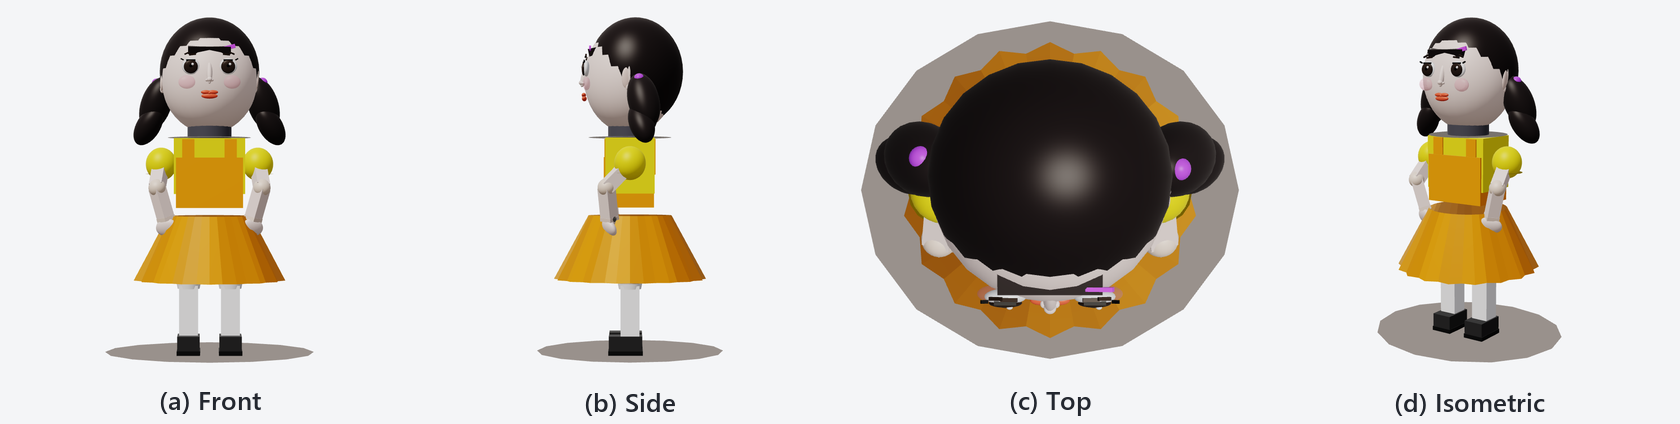
\includegraphics[width=0.84\linewidth]{figures/views_doll.png}
\caption{Young-hee giant doll multi-view projections: (a) Front, (b) Side profile, (c) Top view, (d) Isometric 3D view.}
\end{figure}

\begin{figure}[H]
\centering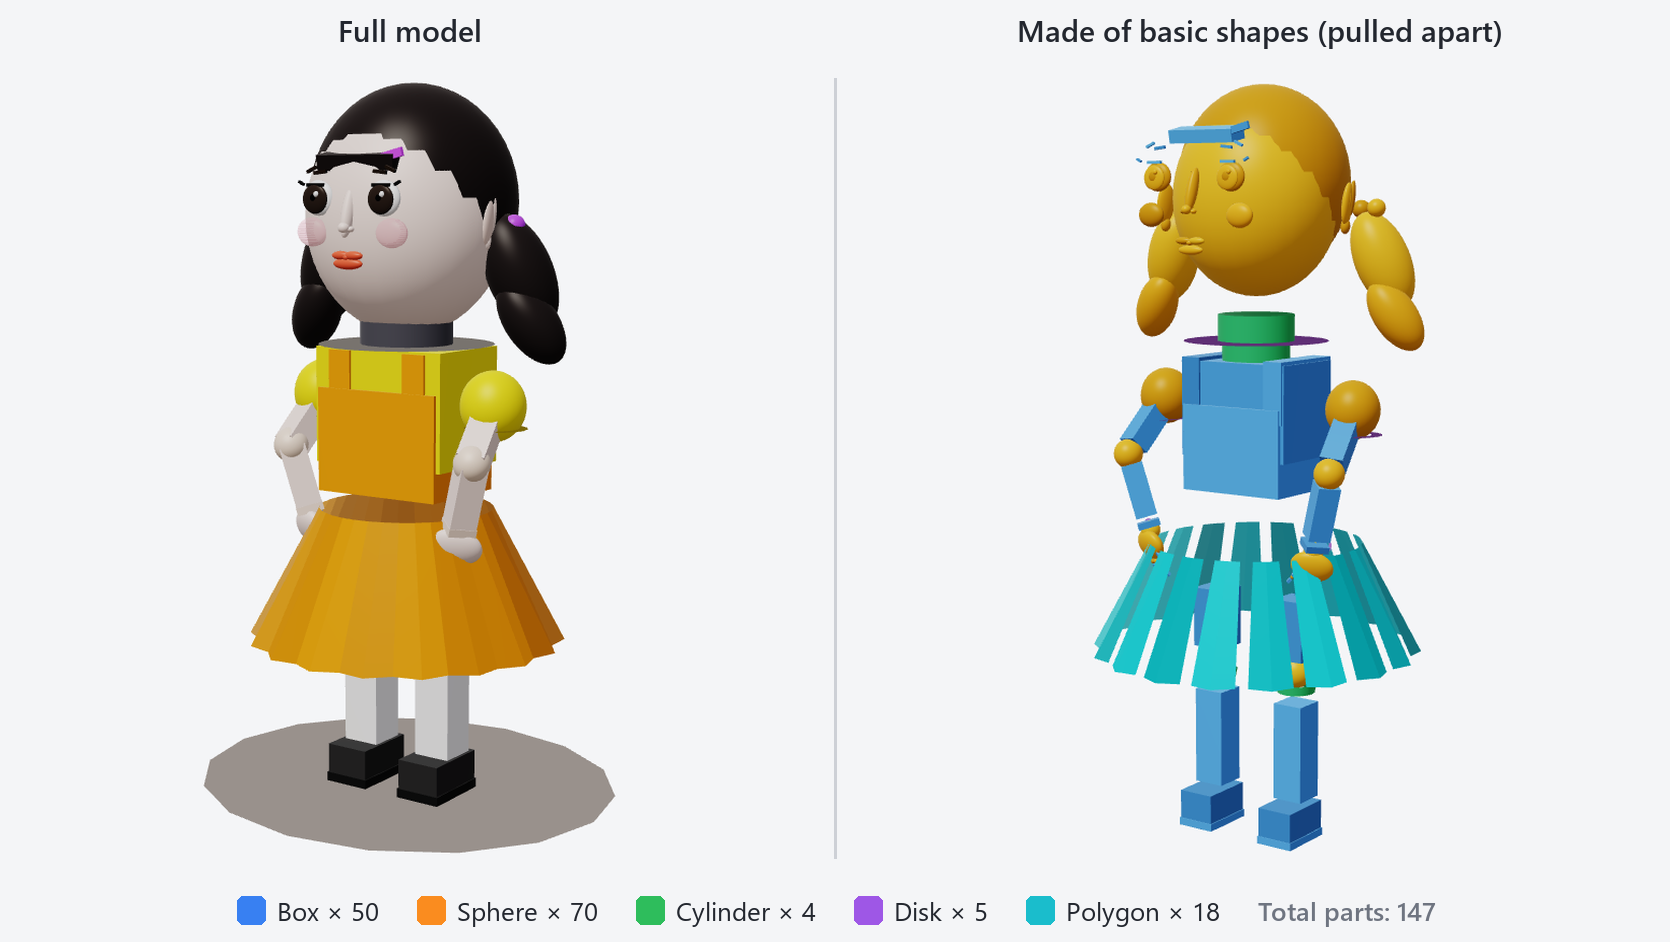
\includegraphics[width=0.50\linewidth]{figures/decomp_doll.png}
\caption{The doll body shape decomposition: 96 parts. The skirt is 18 hand-made polygon pleats.}
\end{figure}

\begin{parttable}
Neck & \shCyl & radius $0.18$, height $0.28$ & $(0,\ 2.05,\ 0)$ & $R_x\,90^\circ$ \\
White collar & \shDsk & radius $0.18\to0.38$ & $(0,\ 1.96,\ 0)$ & $R_x\,90^\circ$ \\
Yellow shirt & \shBox & $0.64\times0.50\times0.44$ & $(0,\ 1.70,\ 0)$ & -- \\
Orange dress top & \shBox & $0.60\times0.45\times0.45$ & $(0,\ 1.55,\ 0.01)$ & -- \\
Dress straps $\times2$ & \shBox & $0.11\times0.32\times0.46$ & $(\pm0.19,\ 1.78,\ 0)$ & -- \\
Pleated skirt & \shPol{} $\times18$ & top radius $0.38$, bottom $0.65$, height $0.58$ & $(0,\ 1.25,\ 0)$ & pleat $i$ at $i\times20^\circ$ \\
Sleeves $\times2$ & \shSph{} + \shDsk & $S(0.14,0.15,0.14)$; ring $0.08\to0.135$ & shoulder $(\pm0.44,\ 1.72,\ 0)$ & cuff $R_x\,90^\circ$ \\
Upper arms $\times2$ & \shBox & $0.12\times0.30\times0.12$ & shoulder $+(0,-0.15,0)$ & $R_x{-46}^\circ R_y{\pm16}^\circ R_z{\pm6}^\circ$ \\
Elbows $\times2$ & \shSph{} + \shBox & radius $0.078$; ring $0.082\times0.02$ & shoulder $+(0,-0.30,0)$ & follows upper arm \\
Forearms $\times2$ & \shBox & $0.115\times0.29\times0.115$ & elbow $+(0,-0.15,0)$ & $R_x58^\circ R_y{\pm34}^\circ R_z{\mp8}^\circ$ \\
Wrists $\times2$ & \shBox{} + \shSph{} + \shDsk & cuff $0.12\times0.035$; ball $r\,0.052$; hole $r\,0.024$ & elbow $+(0,-0.29,0)$ & hole $R_y{\mp90}^\circ$ \\
Palms $\times2$ & \shSph & $S(0.11,0.085,0.045)$ & wrist $+(0,-0.08,0.015)$ & $R_y{\mp24}^\circ R_x12^\circ$ \\
Fingers $\times8$, thumbs $\times2$ & 2 \shSph{} + 2 \shBox{} each & joints $r\,0.010$--$0.014$ & finger $f$ at $x=-0.038+0.025f$ & curl $R_x16^\circ$ \\
Thighs $\times2$ & \shBox & $0.18\times0.32\times0.18$ & $(\pm0.19,\ 0.85,\ 0)$ & -- \\
Knees $\times2$ & \shSph & radius $0.09$ & $(\pm0.19,\ 0.68,\ 0)$ & -- \\
Sock tops $\times2$ & \shCyl & radius $0.11\to0.10$, height $0.05$ & $(\pm0.19,\ 0.64,\ 0)$ & $R_x\,90^\circ$ \\
Socks $\times2$ & \shBox & $0.17\times0.52\times0.17$ & $(\pm0.19,\ 0.36,\ 0)$ & -- \\
Shoes + soles $\times2$ & \shBox{} $\times2$ & $0.20\times0.16\times0.30$; $0.21\times0.04\times0.31$ & $(\pm0.19,\ 0.09,\ 0.04)$; $y{=}0.02$ & -- \\
\end{parttable}

% -------------------------------------------------------------------------------------
\clearpage
\subsection{Young-hee doll head detail}
% -------------------------------------------------------------------------------------
The head rotates independently by $\pm180^\circ$ for player scanning and features dual ocular laser spotlights.
\textbf{Placed with:} local offset $T(0,2.50,0)\cdot R_y(\text{headAngle})$ relative to the torso.

\begin{figure}[H]
\centering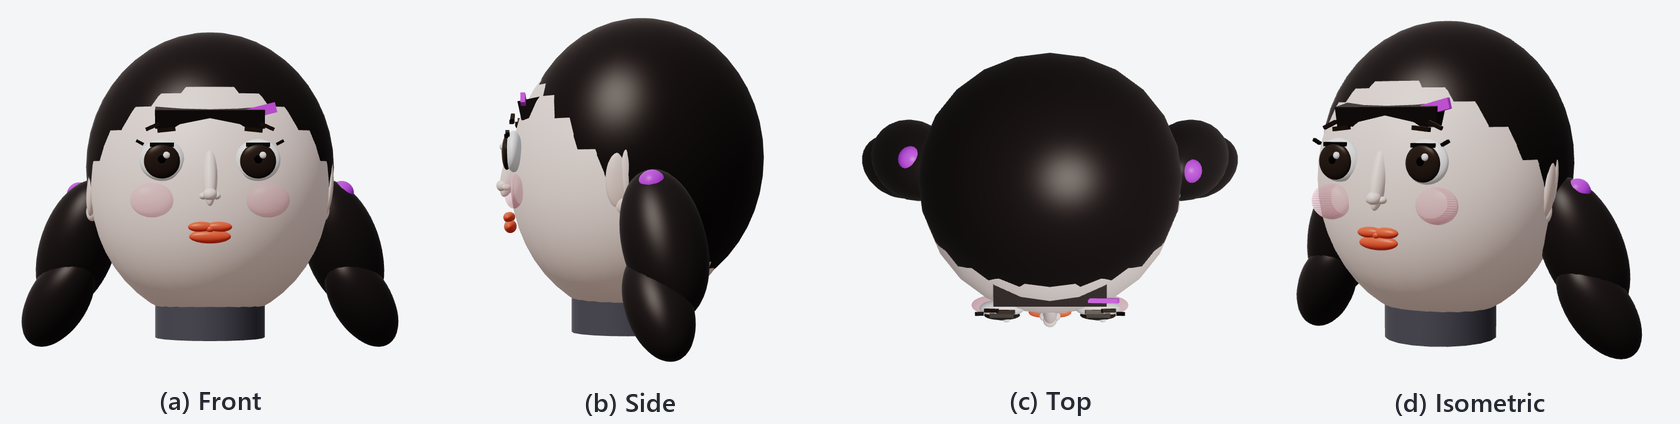
\includegraphics[width=0.84\linewidth]{figures/views_dollhead.png}
\caption{Doll head multi-view projections: (a) Front, (b) Side profile, (c) Top view, (d) Isometric 3D view.}
\end{figure}

\begin{figure}[H]
\centering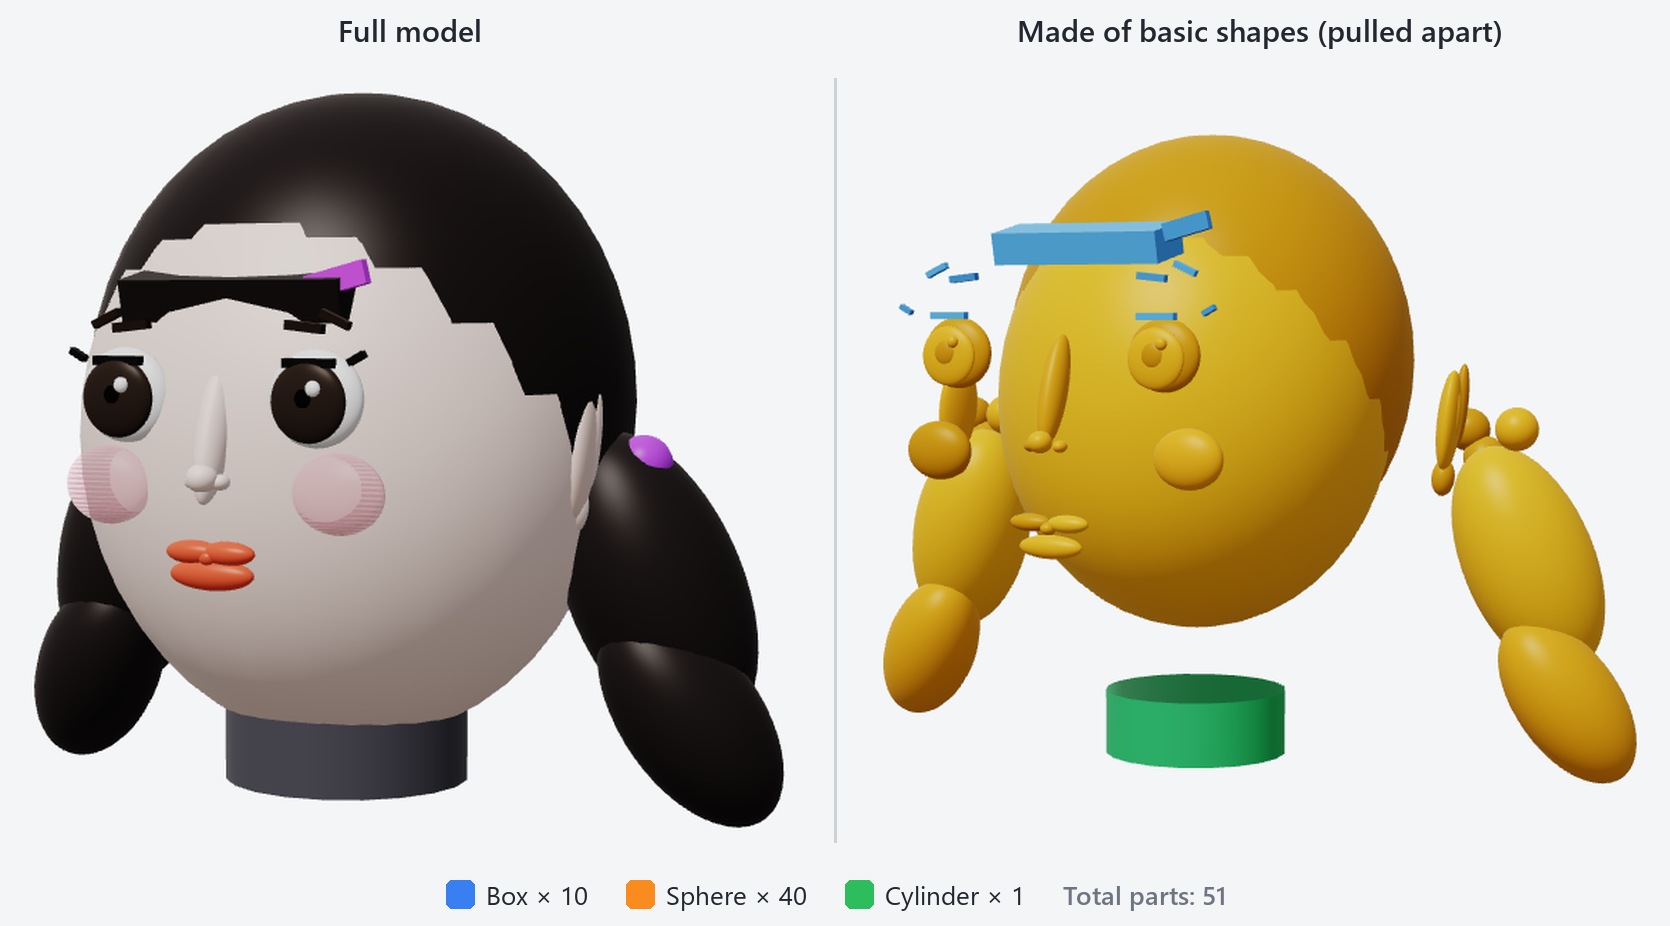
\includegraphics[width=0.50\linewidth]{figures/decomp_dollhead.png}
\caption{The doll's head on its own: 51 parts, mostly squashed spheres.}
\end{figure}

\begin{parttable}
Neck joint ring & \shCyl & radius $0.20$, height $0.14$ & $(0,\ -0.42,\ 0)$ & $R_x\,90^\circ$ \\
Face & \shSph & $S(0.44,0.50,0.42)$ & $(0,\ 0,\ 0)$ & -- \\
Nose bridge, tip & \shSph{} $\times2$ & $S(0.026,0.115,0.034)$; $S(0.024,0.022,0.024)$ & $(0,0.03,0.408)$; $(0,-0.04,0.444)$ & bridge $R_x{-18}^\circ$ \\
Nostrils $\times2$ & \shSph & $S(0.014,0.012,0.016)$ & $(\pm0.023,\ -0.046,\ 0.430)$ & -- \\
Lips (4 parts) & \shSph{} $\times4$ & upper $S(0.046,0.018,0.019)$, lower $S(0.072,0.024,0.022)$ & $(\pm0.030,-0.152,0.422)$, $(0,-0.185,0.418)$ & -- \\
Blush $\times2$ (32\% see-through) & \shSph & $S(0.075,0.060,0.034)$ & $(\pm0.20,\ -0.06,\ 0.392)$ & -- \\
Eyes $\times2$ & 4 \shSph{} + 2 \shBox{} each & white $S(0.078,0.072,0.030)$, iris, pupil, shine, lashes & $(\pm0.165,\ 0.078,\ 0.395)$ & lash wing $R_z{\pm28}^\circ$ \\
Eyebrows $\times2$ & \shBox{} $\times2$ each & $0.062\times0.014$; $0.050\times0.012$ & $(\pm0.150,0.182,0.402)$; $(\pm0.198,0.193,0.397)$ & $R_z{\mp6}^\circ$; $R_z{\mp24}^\circ$ \\
Hair & \shSph & $S(0.455,0.495,0.435)$ & $(0,\ 0.06,\ -0.05)$ & -- \\
Fringe (bangs) & \shBox & $0.38\times0.065\times0.11$ & $(0,\ 0.23,\ 0.32)$ & $R_x12^\circ$ \\
Hair clip & \shBox & $0.10\times0.035\times0.016$ & $(0.18,\ 0.25,\ 0.36)$ & $R_z14^\circ$ \\
Ears $\times2$ & \shSph{} $\times4$ each & main $S(0.024,0.105,0.055)$ & $(\pm0.42,\ -0.02,\ 0.02)$ & $R_y{\pm14}^\circ R_z{-6}^\circ$ \\
Pigtails $\times2$ & \shSph{} $\times6$ each & 4 beads $r\,0.046$; hair $S(0.14,0.26,0.14)$, $S(0.11,0.20,0.11)$ & $(\pm0.44,\ -0.07,\ -0.10)$ & $R_z{\pm20}^\circ$, $R_z{\pm32}^\circ$ \\
Red-light lasers $\times2$ & \shCyl & radius $0.010\to0.07$, length 34 & from each eye, along $+z$ & follows the head \\
\end{parttable}

% -------------------------------------------------------------------------------------
\clearpage
\subsection{The dead tree}
% -------------------------------------------------------------------------------------
The tree is made by a small \emph{recursive} function: a branch draws itself, then two smaller branches at
its tip, and so on. Every branch is a tapered cylinder with a sphere ``knuckle'' at the end, so joints have
no gaps. The bark is a texture (Section~\ref{sec:textures}).
\textbf{Placed with:} $T(0,0,59.85)$, just behind the doll.

\begin{figure}[H]
\centering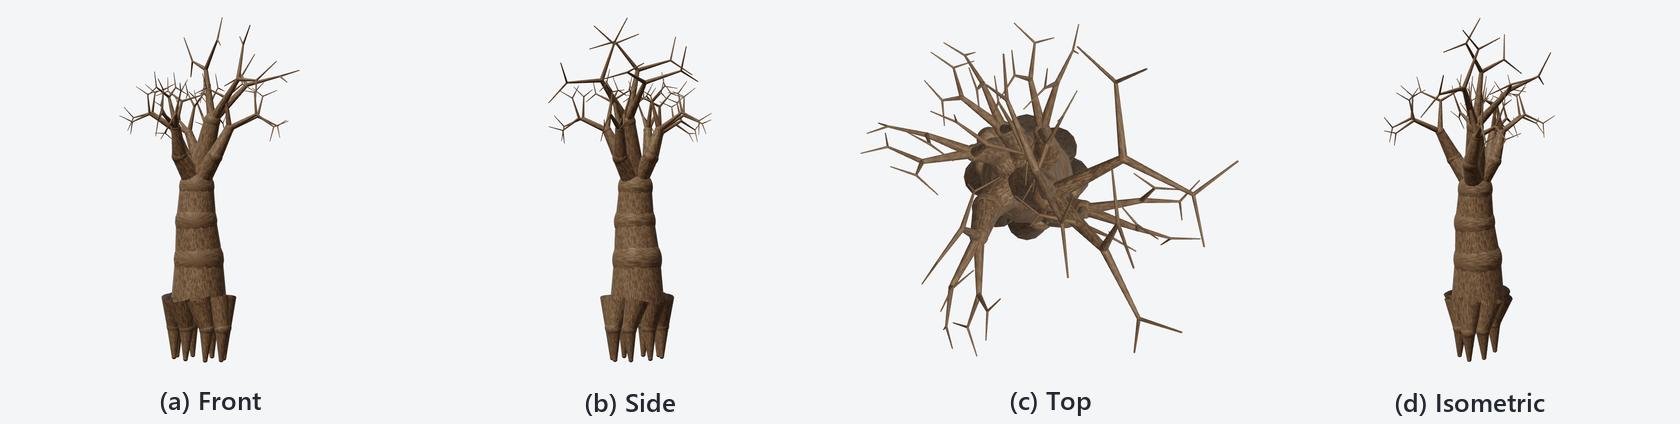
\includegraphics[width=0.84\linewidth]{figures/views_tree.png}
\caption{Dead tree multi-view projections: (a) Front, (b) Side profile, (c) Top view, (d) Isometric 3D view.}
\end{figure}

\begin{figure}[H]
\centering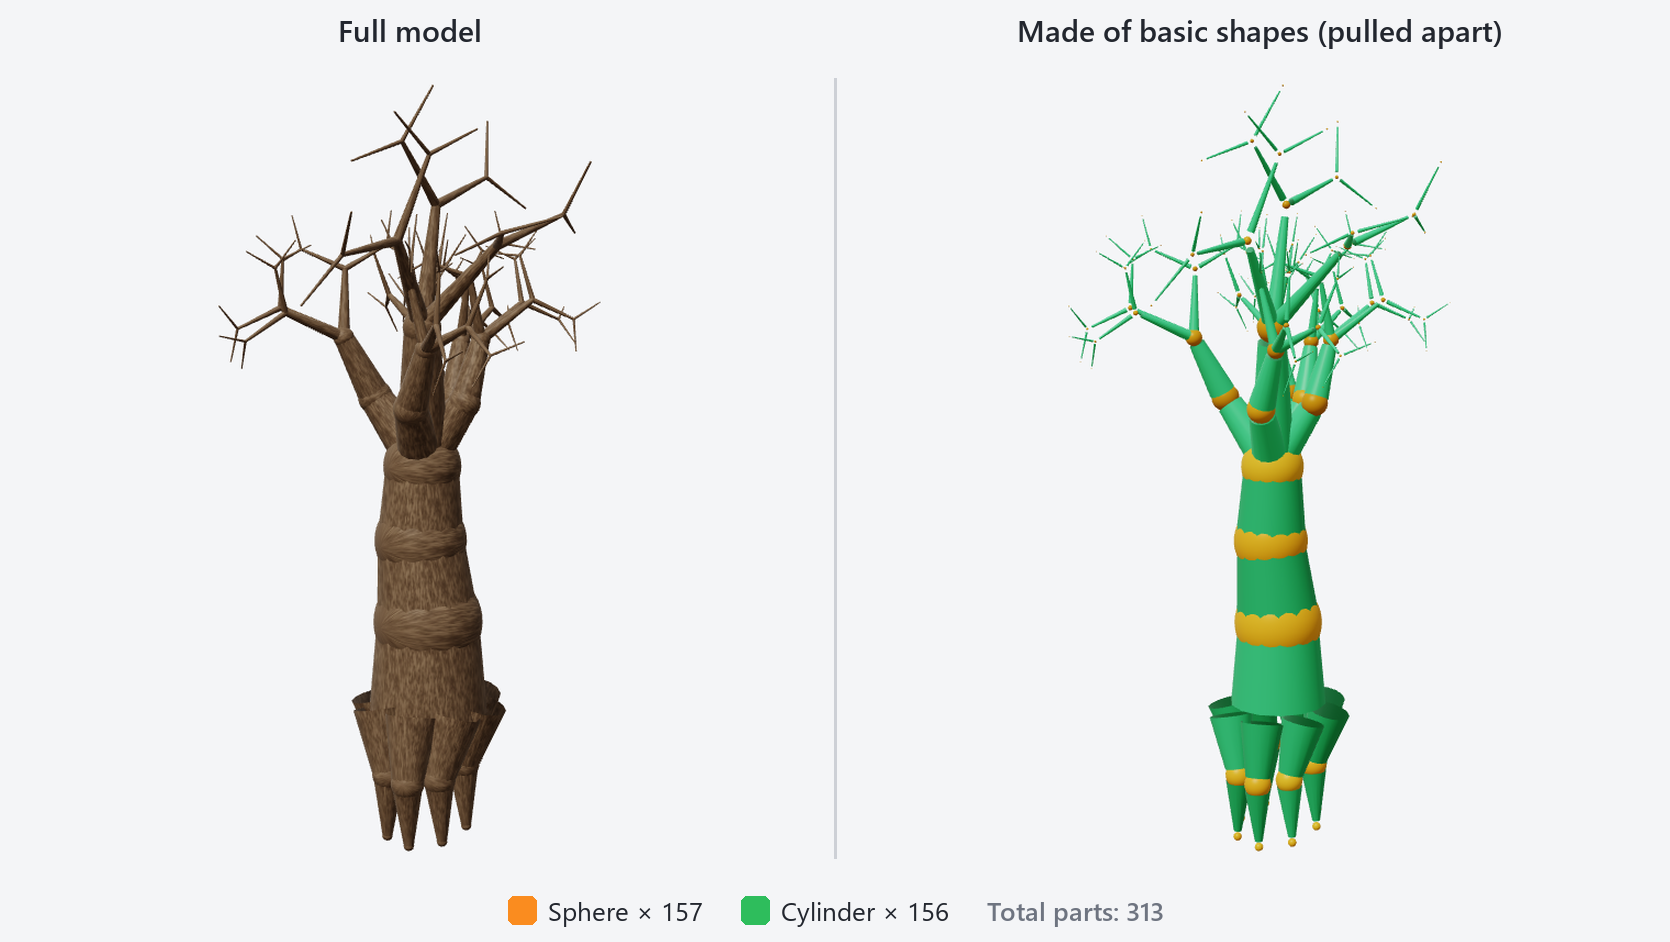
\includegraphics[width=0.50\linewidth]{figures/decomp_tree.png}
\caption{The tree shape decomposition: 156 cylinders and 157 spheres.}
\end{figure}

\begin{parttable}
Roots $\times8$ & 2 \shCyl{} + 2 \shSph{} each & radius $0.65\to0.38\to0.12$, length $1.6+1.6$ & $(1.3\cos\theta,\ 0.25,\ 1.3\sin\theta)$, $\theta=i\cdot45^\circ$ & $R_y\theta\,R_x75^\circ$, then $R_x18^\circ$ \\
Trunk part 1 & \shCyl & radius $1.45\to1.25$, height $2.2$ & $(0,\ 0,\ 0)$ & $R_x{-90}^\circ$ (stand up) \\
Trunk part 2 & \shCyl & radius $1.25\to1.05$, height $2.0$ & on top of part 1 & $R_x3.5^\circ R_y{-4}^\circ$ \\
Trunk part 3 & \shCyl & radius $1.05\to0.88$, height $1.8$ & on top of part 2 & $R_x{-4.5}^\circ R_y5^\circ$ \\
Fork knuckle & \shSph & radius $0.92$ & top of trunk ($\approx6$ high) & -- \\
Big branches $\times5$ & 2 \shCyl{} + 3 twigs each & base radius $0.50$--$0.56$, length $3.2$--$3.6$ & at the fork & $R_z$: $-48^\circ, 48^\circ, -135^\circ, 135^\circ, 180^\circ$; $R_x$: $28^\circ$--$38^\circ$ \\
Top spire & \shCyl{} + 3 twigs & radius $0.65\to0.42$, length $3.5$ & at the fork & $R_x8^\circ R_y12^\circ$ \\
Twigs (recursive) & \shCyl{} + \shSph & each level: length $\times0.70$, radius $\times0.45$ & at the parent's tip & $R_y\pm(26^\circ$--$40^\circ)$, $R_x\pm(35^\circ$--$70^\circ)$ \\
\end{parttable}

% -------------------------------------------------------------------------------------
\clearpage
\subsection{Village house}
% -------------------------------------------------------------------------------------
One house model is drawn 9 times: five in a row behind the start ($z=-67$) and two on each side wall
($x=\pm22$, turned $\pm90^\circ$). \textbf{Placed with:} $T(x,0,z)\cdot R_y(\text{angle})$.

\begin{figure}[H]
\centering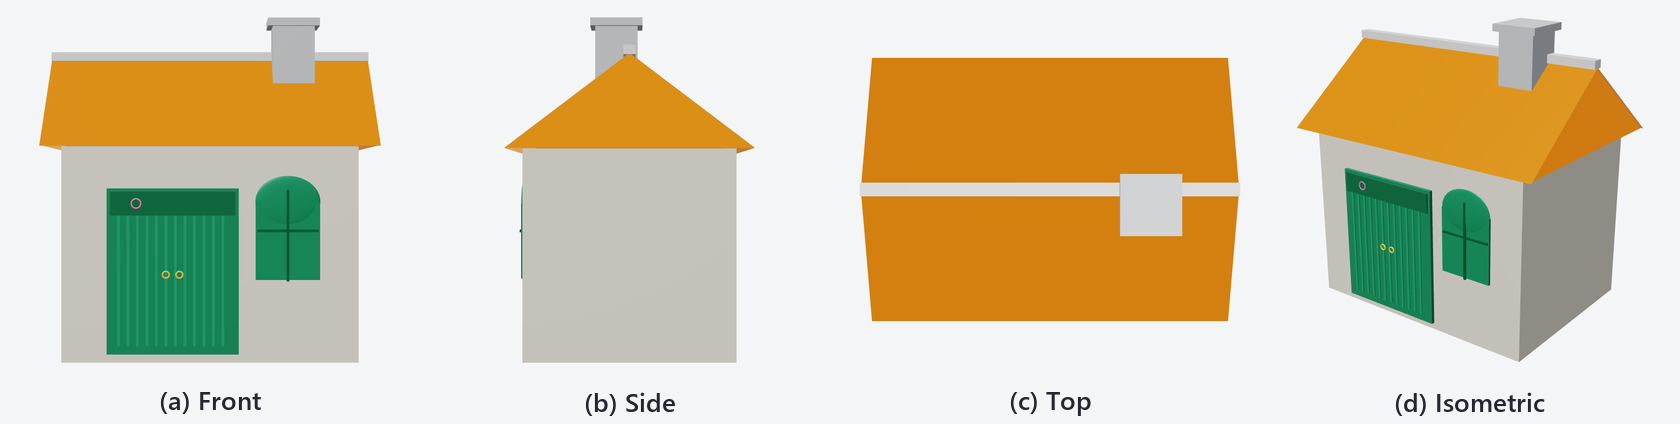
\includegraphics[width=0.84\linewidth]{figures/views_house.png}
\caption{Village house multi-view projections: (a) Front, (b) Side profile, (c) Top view, (d) Isometric 3D view.}
\end{figure}

\begin{figure}[H]
\centering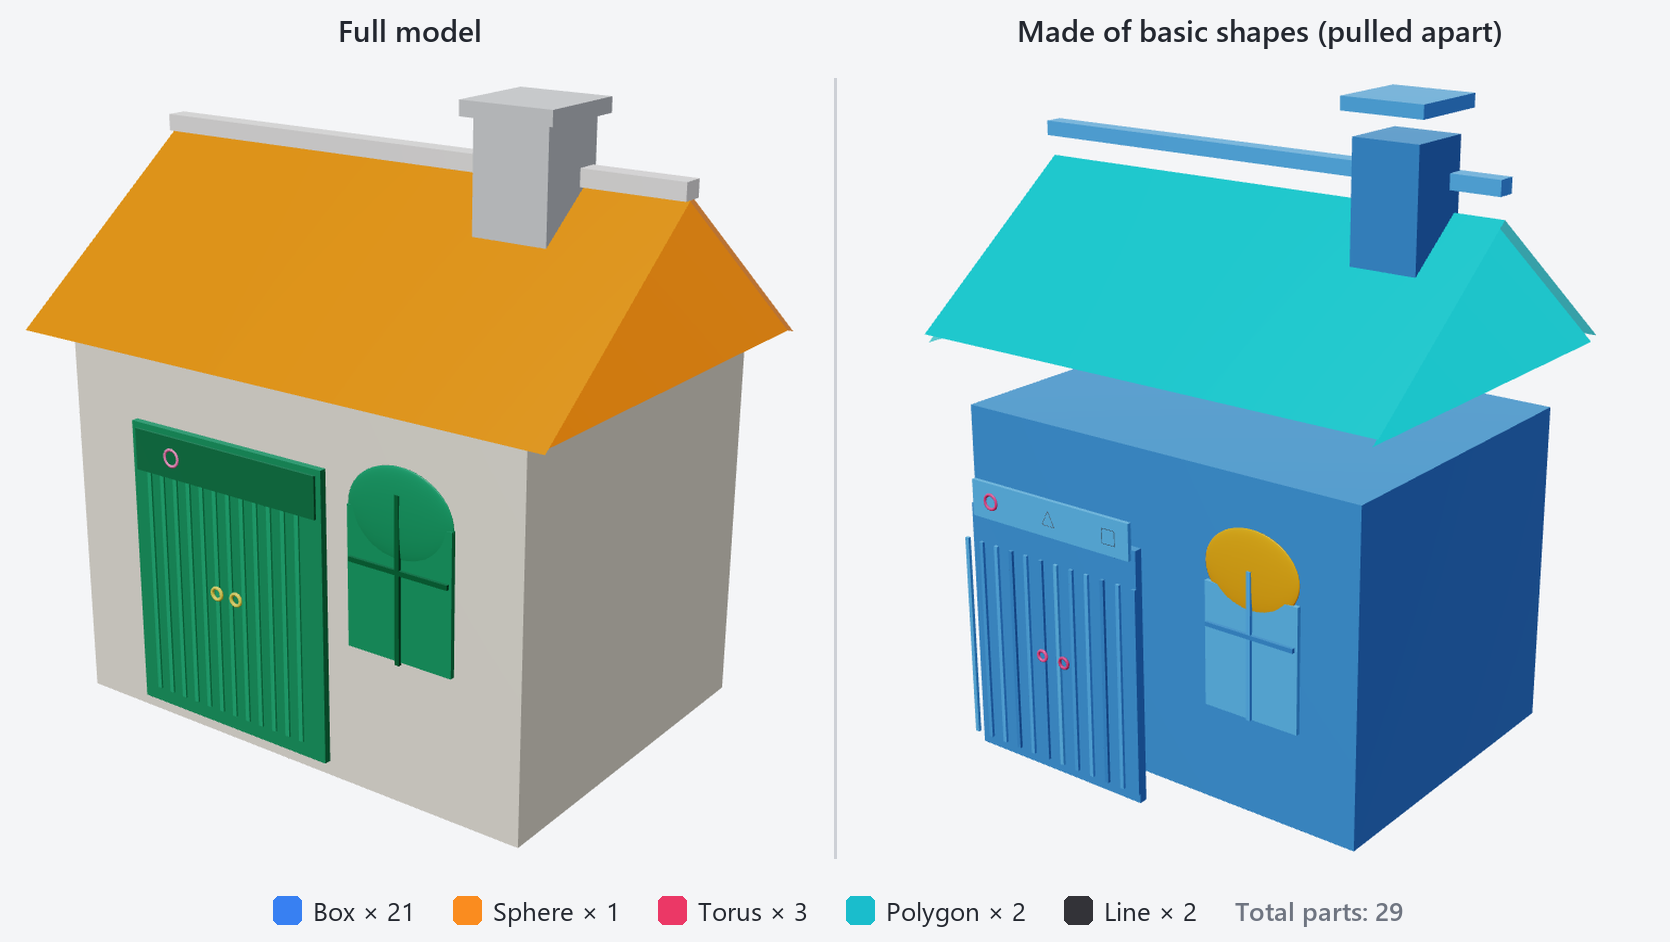
\includegraphics[width=0.50\linewidth]{figures/decomp_house.png}
\caption{Village house shape decomposition: 29 parts. The roof is made of hand-made triangles and quads.}
\end{figure}

\begin{parttable}
Walls (body) & \shBox & $4.4\times3.2\times3.2$ & $(0,\ 1.6,\ 0)$ & -- \\
Roof ends $\times2$ & \shPol{} (triangle) & base $3.7$, height $1.4$ & $x=\pm2.45$, from $y=3.2$ & normal $(\pm0.71,0.71,0)$ \\
Roof sides $\times2$ & \shPol{} (quad) & $5.0$ long, $1.85$ deep, $1.4$ rise & front / back, from $y=3.2$ & normal $(0,0.71,\pm0.71)$ \\
Roof ridge & \shBox & $5.0\times0.14\times0.18$ & $(0,\ 4.65,\ 0)$ & -- \\
Chimney + cap & \shBox{} $\times2$ & $0.65\times1.4\times0.65$; $0.80\times0.12\times0.80$ & $(1.3,\ 4.4,\ 0.2)$; $(1.3,\ 5.15,\ 0.2)$ & -- \\
Door frame & \shBox & $1.95\times2.45\times0.08$ & $(-0.55,\ 1.35,\ 1.62)$ & -- \\
Door bars $\times12$ & \shBox & $0.04\times2.0\times0.03$ & $x=-1.35$ to $0.19$, every $0.14$ & -- \\
Sign above door & \shBox & $1.85\times0.35\times0.04$ & $(-0.55,\ 2.35,\ 1.66)$ & -- \\
Symbols $\bigcirc\,\triangle\,\square$ & \shTor{} + 2 line loops & ring $0.07$; triangle/square $0.14$ wide & on the sign & -- \\
Door rings $\times2$ & \shTor & tube $0.015$, ring $0.05$ & $(-0.65,\ 1.30,\ 1.68)$, $(-0.45,\ 1.30,\ 1.68)$ & -- \\
Window + round top & \shBox{} + \shSph & $0.95\times1.15\times0.04$; $S(0.48,0.38,0.04)$ & $(1.15,\ 1.8,\ 1.64)$; $+(0,0.58,0)$ & -- \\
Window bars $\times2$ & \shBox & $0.04\times1.35$; $0.90\times0.04$ & window $+(0,0.08,0.03)$, $+(0,0.15,0.03)$ & -- \\
\end{parttable}

% % -------------------------------------------------------------------------------------
\clearpage
\subsection{Countdown clock}
% -------------------------------------------------------------------------------------
A digital clock hangs above the finish line and shows the remaining game time on both sides.
Each digit is formed using 7-segment digital bars, updated synchronously each second.
\textbf{Placed with:} $T(0,17.5,42)\cdot S(2)$.

\begin{figure}[H]
\centering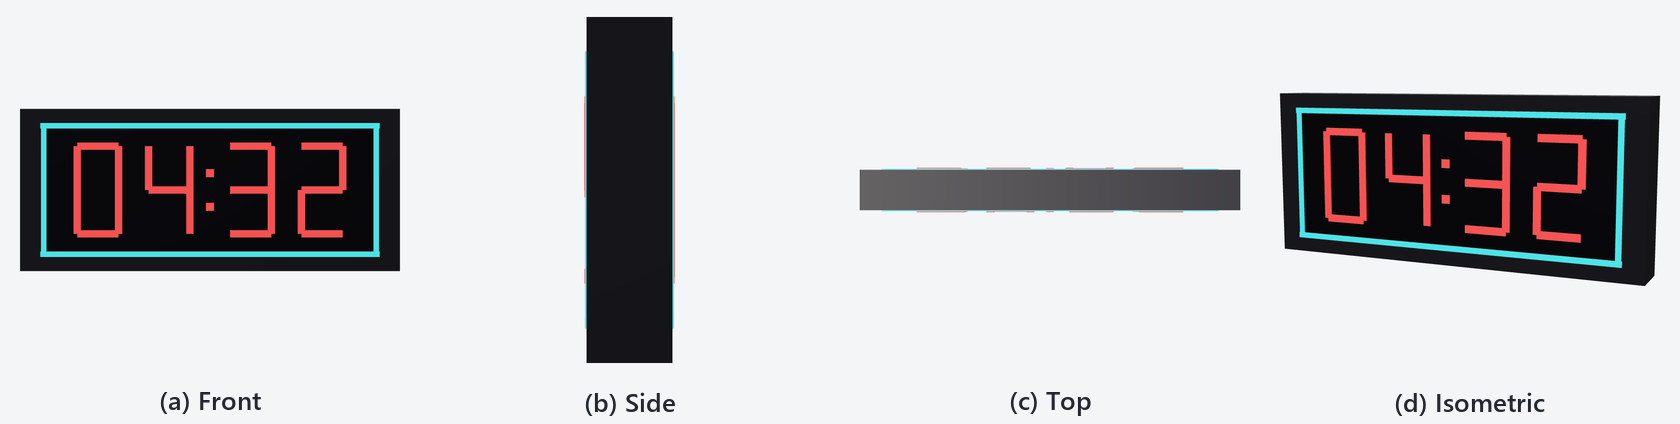
\includegraphics[width=0.92\linewidth]{figures/views_clock.png}
\caption{Countdown scoreboard clock multi-view projections: (a) Front, (b) Side profile, (c) Top view, (d) Isometric 3D view.}
\end{figure}

\begin{figure}[H]
\centering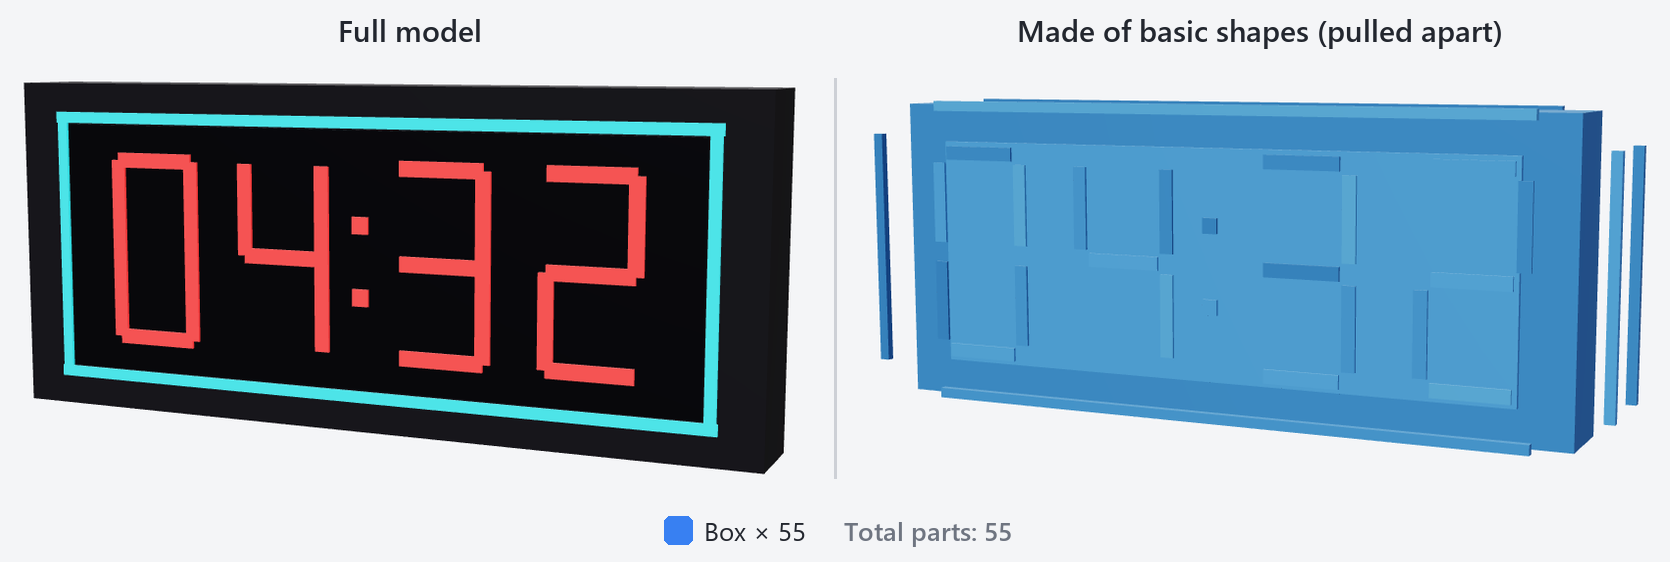
\includegraphics[width=0.62\linewidth]{figures/decomp_clock.png}
\caption{Clock showing 04:32: 55 boxes.}
\end{figure}

\begin{parttable}
Outer frame & \shBox & $5.6\times2.4\times0.6$ & $(0,\ 0,\ 0)$ & -- \\
Glowing border $\times4$ (each side) & \shBox & $5.0\times0.08\times0.06$, $0.08\times1.9\times0.06$ & $y=\pm0.95$; $x=\pm2.45$; $z=\pm0.29$ & -- \\
Black screen (each side) & \shBox & $4.8\times1.8\times0.04$ & $(0,\ 0,\ \pm0.29)$ & -- \\
Digit bars (each digit) & \shBox{} $\times$ up to 7 & across $0.61\times0.11$, up $0.11\times0.65$ & digits at $x=\pm1.65,\ \pm0.60$ & back side mirrored \\
Colon dots $\times2$ (each side) & \shBox & $0.12\times0.12\times0.02$ & $(0,\ \pm0.25,\ \pm0.33)$ & -- \\
\end{parttable}
\note{Seven-segment bitmasks: $A$ (top), $B$ (top-right), $C$ (bottom-right), $D$ (bottom), $E$ (bottom-left), $F$ (top-left), $G$ (mid). Digits are updated via bitwise masks (\texttt{0x3F} for 0, \texttt{0x7F} for 8).}

% -------------------------------------------------------------------------------------
\clearpage
\subsection{The glass bridge}
% -------------------------------------------------------------------------------------
The bridge is entirely boxes. Step $i$ ($i=0..15$) is at $z_i = 3 + 3.3\,i$, at height 16.
The full bridge is $54.3$ long ($z$ from $2.0$ to $56.3$, centre $29.15$).

\begin{figure}[H]
\centering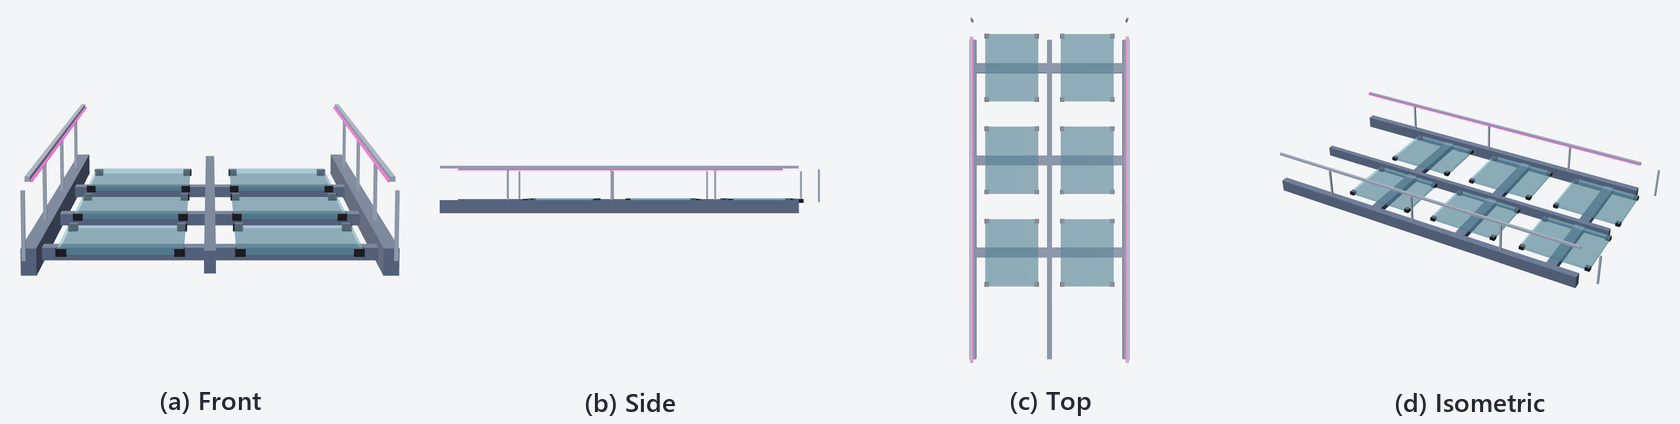
\includegraphics[width=0.88\linewidth]{figures/views_bridge.png}
\caption{Glass bridge stepping stone multi-view projections: (a) Front, (b) Side profile, (c) Top view, (d) Isometric 3D view.}
\end{figure}

\begin{figure}[H]
\centering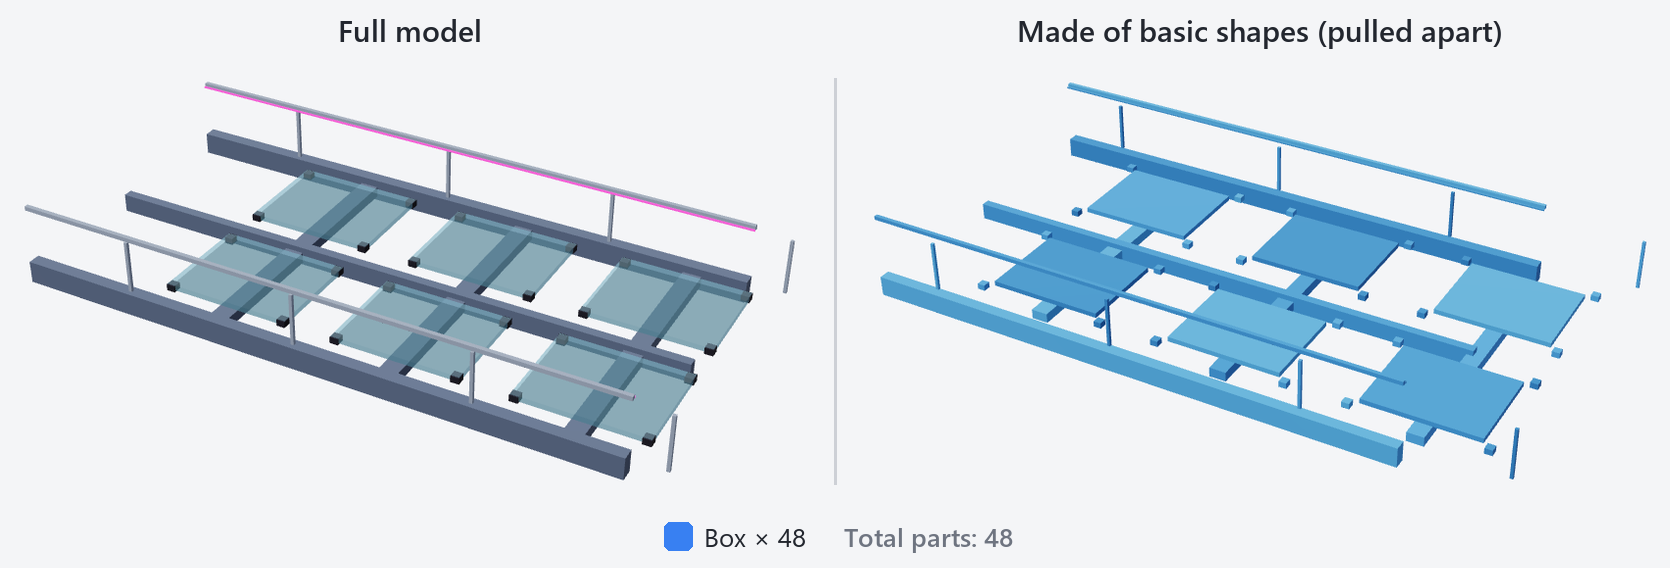
\includegraphics[width=0.56\linewidth]{figures/decomp_bridge.png}
\caption{The first 3 steps of the bridge: 48 boxes (the full 16-step bridge uses 217).}
\end{figure}

\begin{parttable}
Steel beams $\times2$ & \shBox & $0.24\times0.42\times54.3$ & $(\pm2.75,\ 15.78,\ 29.15)$ & -- \\
Hand rails $\times2$ & \shBox & $0.08\times0.08\times54.3$ & $(\pm2.75,\ 17.05,\ 29.15)$ & -- \\
Pink neon strips $\times2$ & \shBox{} (glowing) & $0.03\times0.03\times54.3$ & $(\pm2.69,\ 17.02,\ 29.15)$ & -- \\
Rail posts $\times34$ & \shBox & $0.06\times1.05\times0.06$ & $(\pm2.75,\ 16.45,\ z_i-1.65)$ & -- \\
Middle beam & \shBox & $0.18\times0.35\times54.3$ & $(0,\ 15.78,\ 29.15)$ & -- \\
Cross beams $\times16$ & \shBox & $5.6\times0.20\times0.35$ & $(0,\ 15.75,\ z_i)$ & -- \\
Glass panes $\times32$ & \shBox{} (42\% see-through) & $1.90\times0.10\times2.40$ & $(\pm1.35,\ 15.98,\ z_i)$ & -- \\
Corner clamps $\times128$ & \shBox & $0.16\times0.12\times0.16$ & pane $+(\pm0.89,\ -0.06,\ \pm1.13)$ & -- \\
``Safe'' green glow & \shBox{} (glowing) & $1.82\times0.02\times2.30$ & just above a proven pane & -- \\
Broken pane marks & \shBox{} $\times4$ & $0.24\times0.02\times0.24$ (red) & at the four corners & -- \\
\end{parttable}
\note{Step pairs are generated along $+z$. Alpha blending ($\alpha=0.42$) uses \texttt{glDepthMask(GL\_FALSE)} during transparent rendering to maintain proper depth order.}

% -------------------------------------------------------------------------------------
\clearpage
\subsection{Glass bridge start platform}
% -------------------------------------------------------------------------------------
\textbf{Start platform placed with:} $T(0,\ 15.75,\ -4.5)$. The finish platform is the same idea at the other
end ($z=61$), without rails. The deck uses the concrete texture.

\begin{figure}[H]
\centering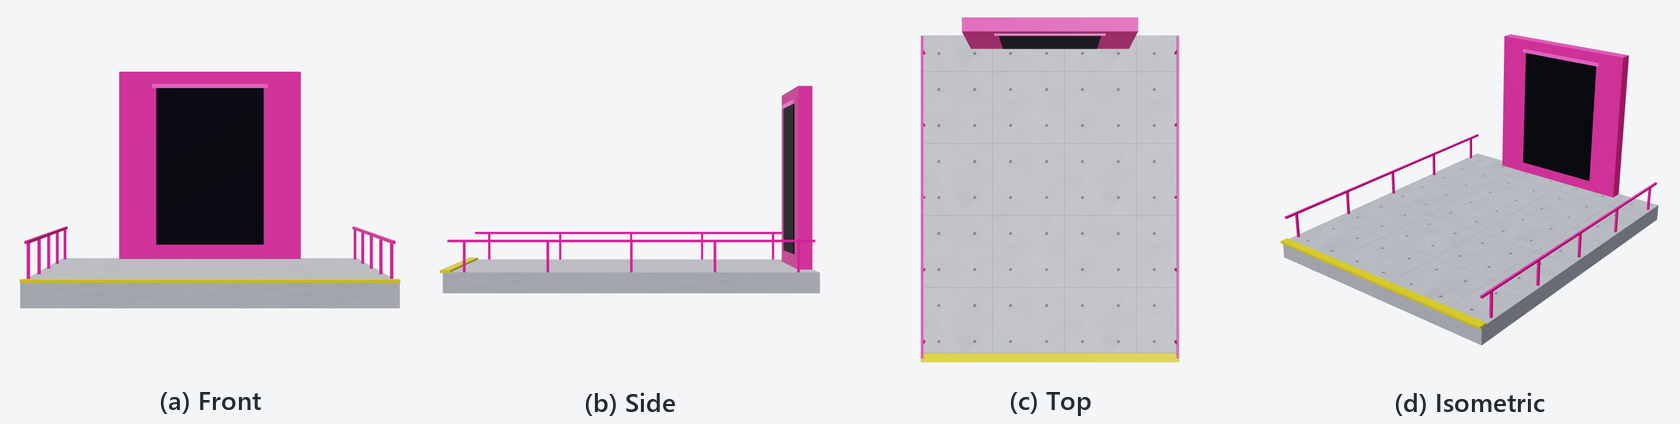
\includegraphics[width=0.92\linewidth]{figures/views_platform.png}
\caption{Glass bridge start platform multi-view projections: (a) Front, (b) Side profile, (c) Top view, (d) Isometric 3D view.}
\end{figure}

\begin{figure}[H]
\centering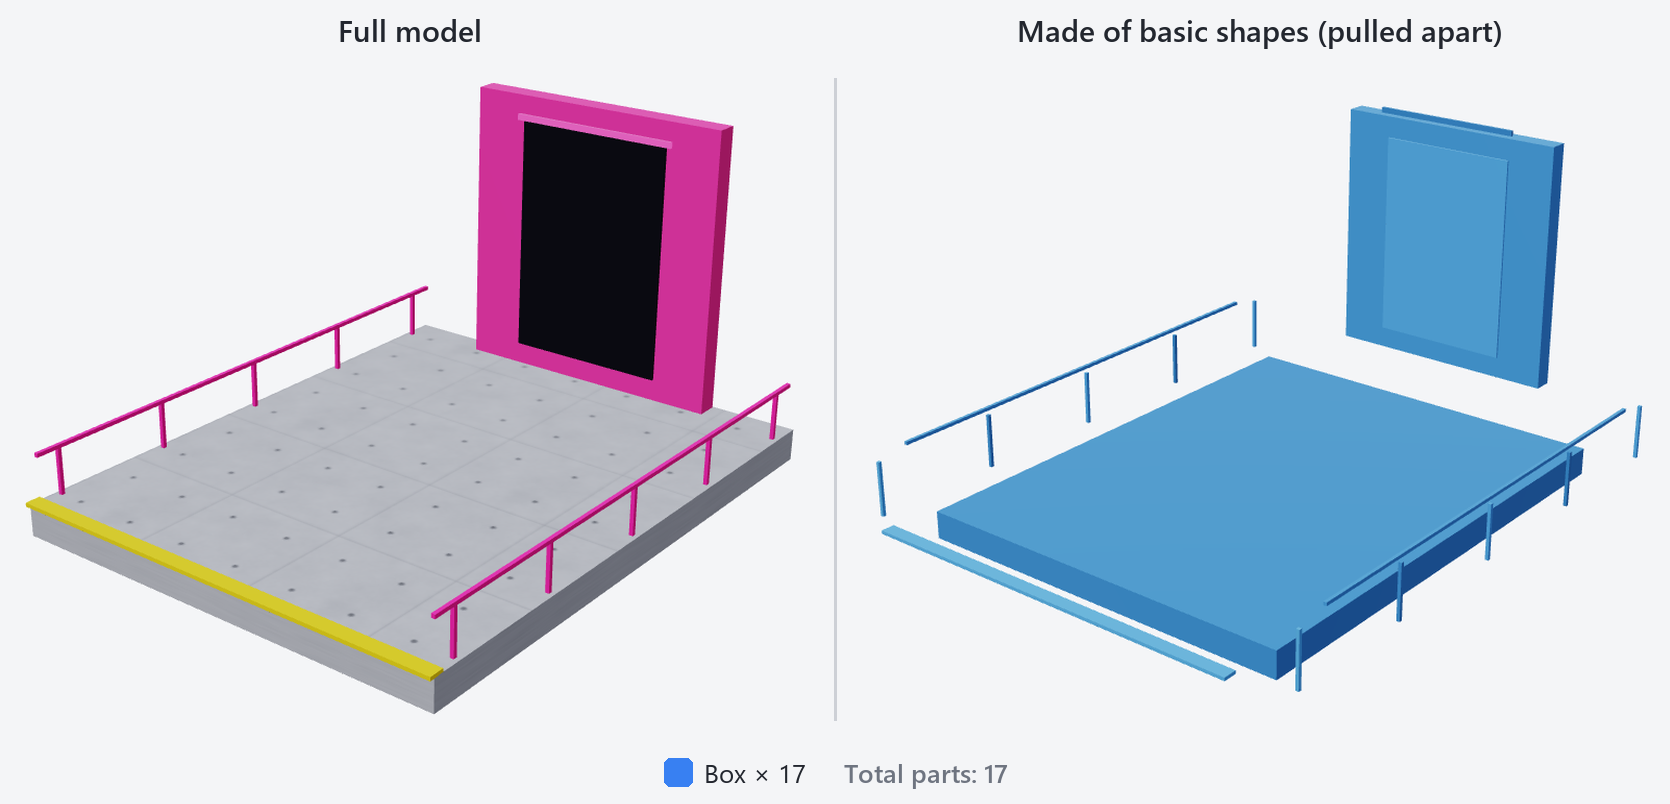
\includegraphics[width=0.62\linewidth]{figures/decomp_platform.png}
\caption{Start platform with its exit door: 17 boxes.}
\end{figure}

\begin{parttable}
Concrete deck & \shBox{} (textured) & $7.2\times0.5\times9.0$ & $(0,\ 0,\ 0)$ & -- \\
Yellow edge & \shBox & $7.2\times0.06\times0.25$ & $(0,\ 0.27,\ 4.45)$ & -- \\
Top rails $\times2$ & \shBox & $0.06\times0.06\times8.8$ & $(\pm3.5,\ 1.0,\ 0)$ & -- \\
Rail posts $\times10$ & \shBox & $0.06\times1.0\times0.06$ & $(\pm3.5,\ 0.5,\ -4,-2,0,2,4)$ & -- \\
Door frame & \shBox & $4.4\times4.6\times0.35$ & $(0,\ 2.5,\ -4.3)$ & -- \\
Dark doorway & \shBox & $2.6\times3.8\times0.42$ & $(0,\ 2.5,\ -4.3)$ & -- \\
Glowing strip & \shBox{} (glowing) & $2.8\times0.10\times0.05$ & door $+(0,\ 1.95,\ 0.22)$ & -- \\
\end{parttable}
\note{The platform anchors contestants at height $y=15.75$ prior to step 1. Bounding box collision restricts premature lateral movement before the round begins.}

% -------------------------------------------------------------------------------------
\clearpage
\subsection{Round 2 bridge guard}
% -------------------------------------------------------------------------------------
Four guards stand watch on the elevated platforms, equipped with rifles and standard geometric uniform harnesses.
\textbf{Placed with:} $T(x,16,z)\cdot R_y(\text{angle})$: two guards at the start ($x=\pm2.4$, angles $\pm30^\circ$) and two at the finish.

\begin{figure}[H]
\centering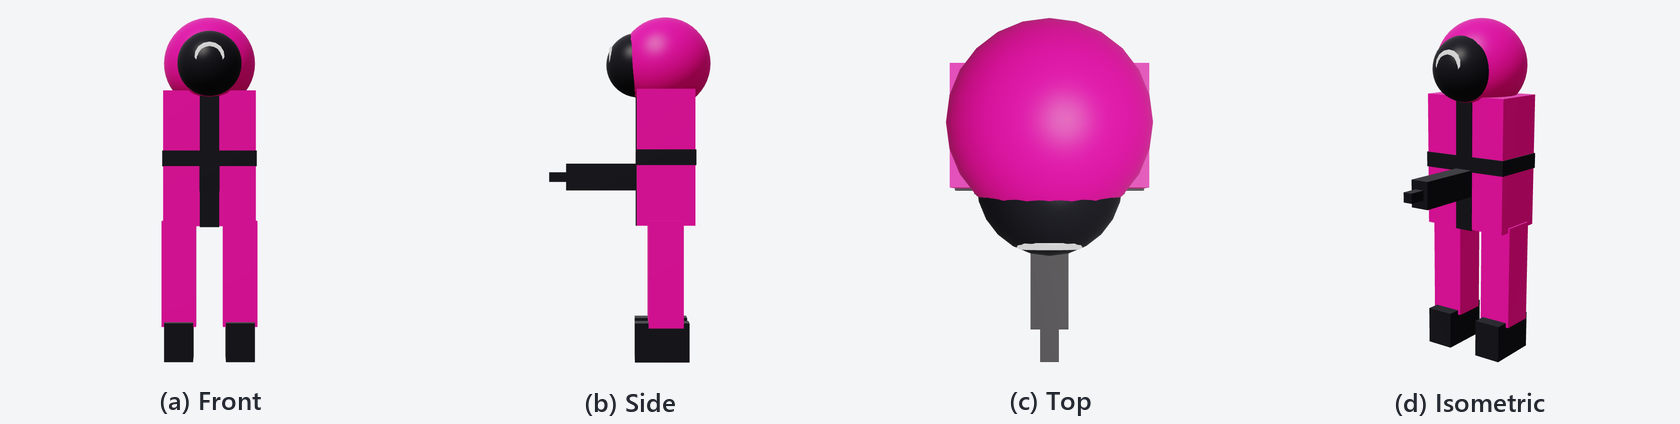
\includegraphics[width=0.92\linewidth]{figures/views_gbguard.png}
\caption{Round 2 bridge guard multi-view projections: (a) Front, (b) Side profile, (c) Top view, (d) Isometric 3D view.}
\end{figure}

\begin{figure}[H]
\centering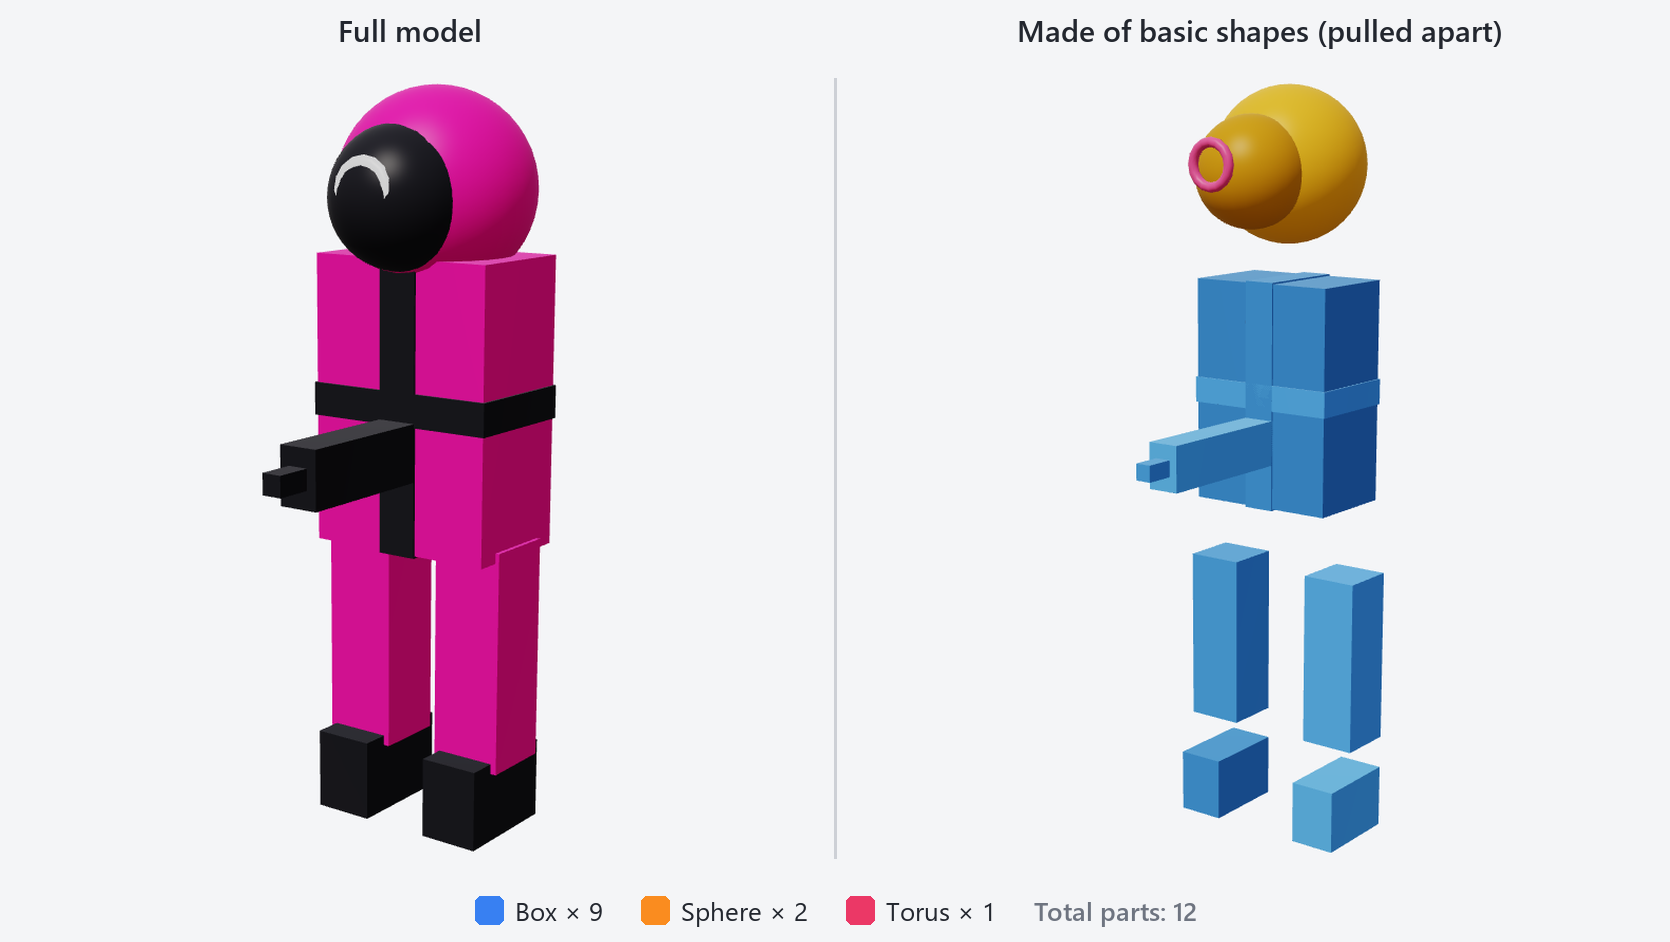
\includegraphics[width=0.62\linewidth]{figures/decomp_gbguard.png}
\caption{Bridge guard (simpler than the Round 1 guard): 9 boxes, 2 spheres, 1 torus.}
\end{figure}

\begin{parttable}
Boots $\times2$ & \shBox & $0.15\times0.20\times0.28$ & $(\pm0.16,\ 0.10,\ 0.02)$ & -- \\
Legs $\times2$ & \shBox & $0.18\times0.55\times0.18$ & $(\pm0.16,\ 0.45,\ 0)$ & -- \\
Body, belt, strap & \shBox{} $\times3$ & $0.48\times0.70\times0.30$; $0.49\times0.08$; $0.10\times0.71$ & $(0,\ 1.05,\ 0)$ & -- \\
Rifle & \shBox{} $\times2$ & $0.10\times0.14\times0.52$; $0.05\times0.05\times0.70$ & $(0,\ 0.95,\ 0.26)$ & -- \\
Head, mask & \shSph{} $\times2$ & radius $0.24$; $0.17$ & $(0,\ 1.55,\ 0)$; $(0,\ 1.54,\ 0.14)$ & -- \\
Circle symbol & \shTor & tube $0.015$, ring $0.065$ & mask $+(0,\ 0.02,\ 0.14)$ & -- \\
\end{parttable}
\note{Bridge overseers feature circle rank emblems on their masks and carry low-poly rifles angled at $R_y\,\mp30^\circ$ toward the contestants.}

% -------------------------------------------------------------------------------------
\clearpage
\subsection{Light fixtures}
% -------------------------------------------------------------------------------------
Each light source in the simulation features a visible geometric housing rendering its physical presence.
\begin{figure}[H]
\centering
\begin{subfigure}{0.48\linewidth}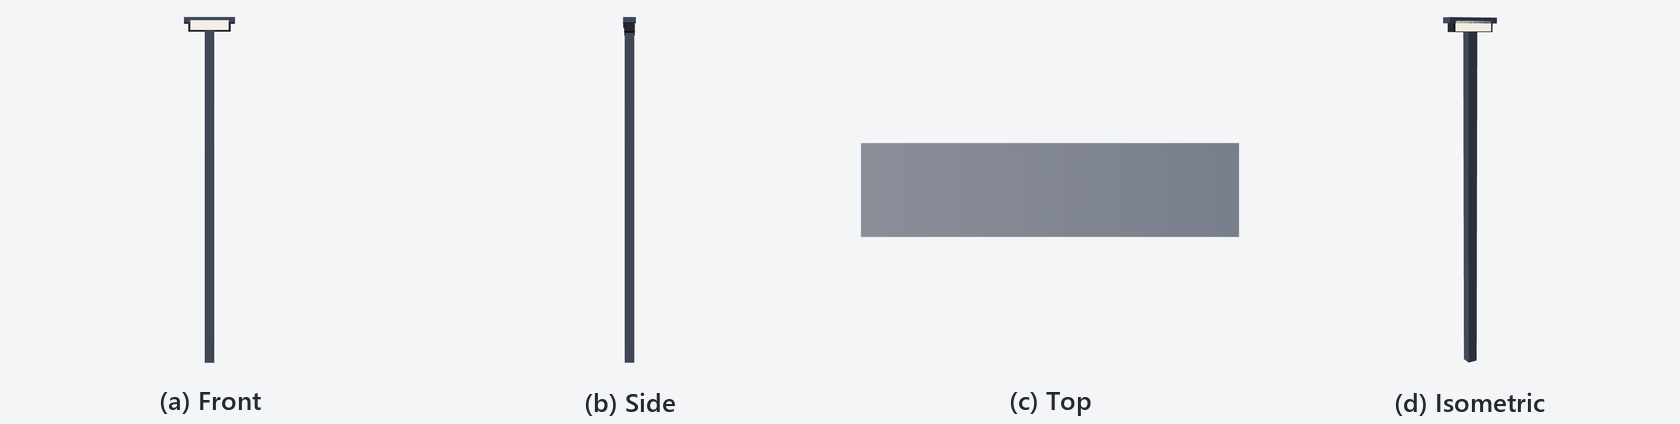
\includegraphics[width=\linewidth]{figures/views_floodlight.png}\caption{Floodlight tower (Round 1)}\end{subfigure}\hfill
\begin{subfigure}{0.48\linewidth}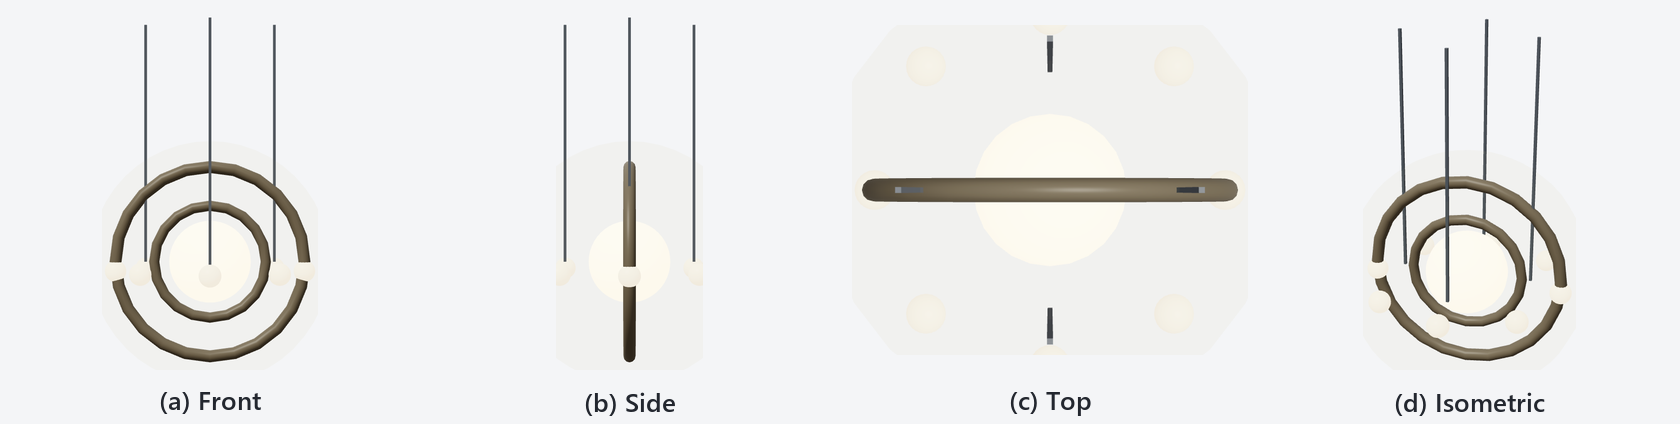
\includegraphics[width=\linewidth]{figures/views_chandelier.png}\caption{Bridge chandelier (Round 2)}\end{subfigure}
\caption{Light fixtures multi-view projections: (a) Front, (b) Side, (c) Top, (d) Isometric.}
\end{figure}

\begin{figure}[H]
\centering
\begin{subfigure}{0.31\linewidth}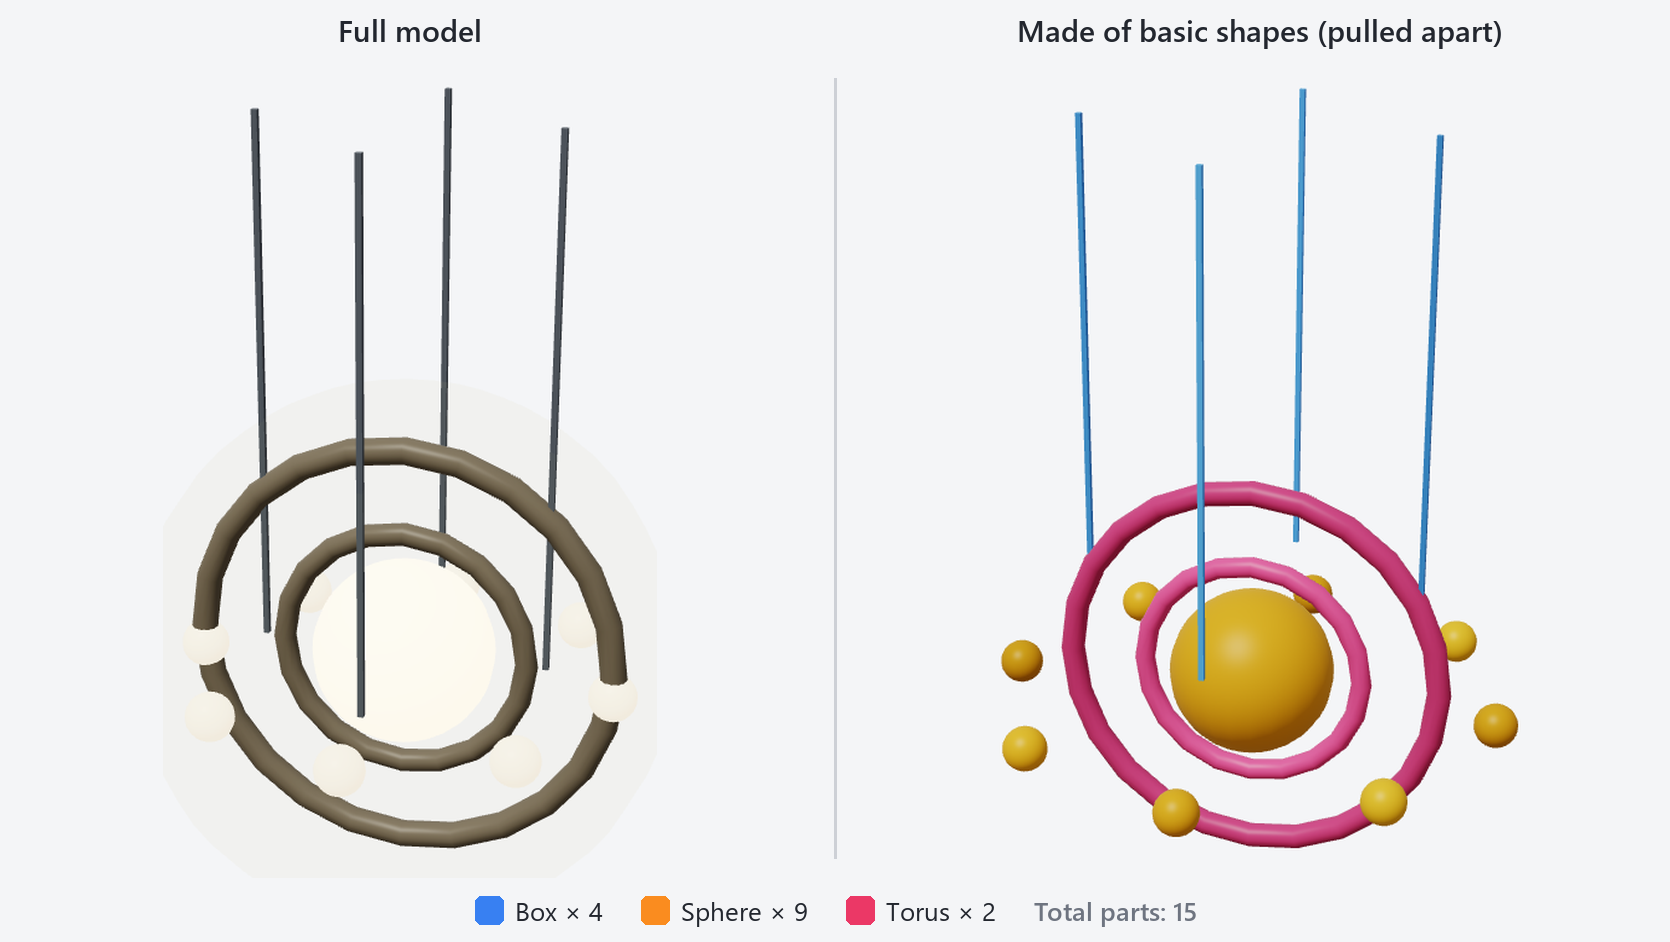
\includegraphics[width=\linewidth]{figures/decomp_chandelier.png}
\caption{Chandelier (point)}\end{subfigure}\hfill
\begin{subfigure}{0.31\linewidth}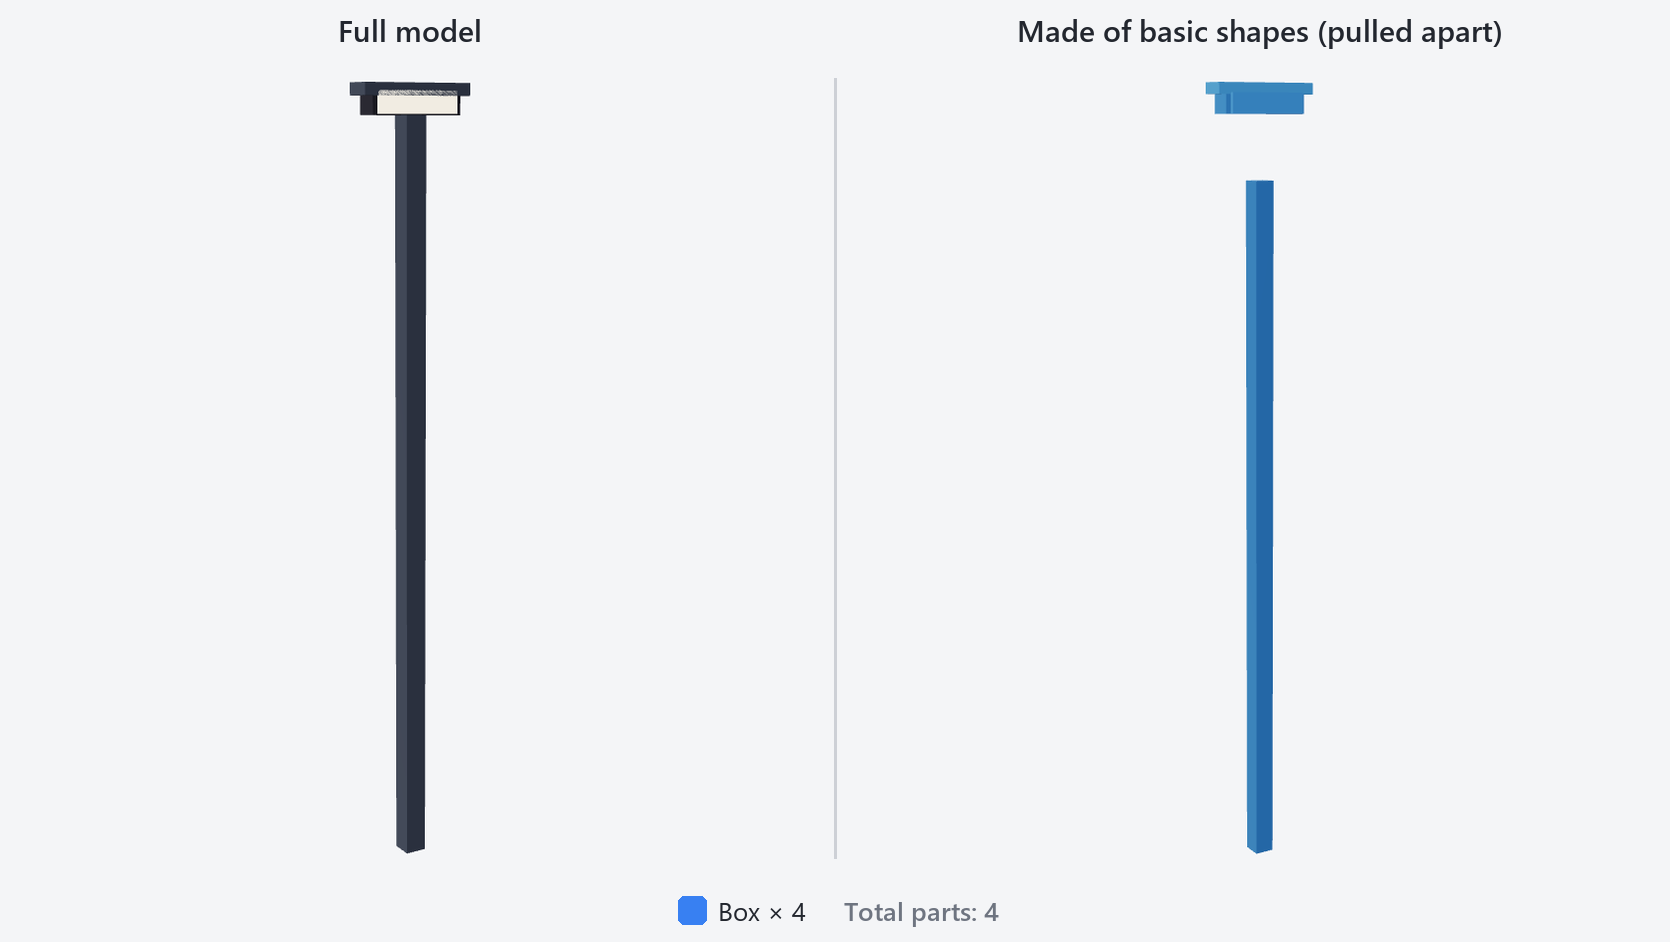
\includegraphics[width=\linewidth]{figures/decomp_floodlight.png}
\caption{Tower (point)}\end{subfigure}\hfill
\begin{subfigure}{0.31\linewidth}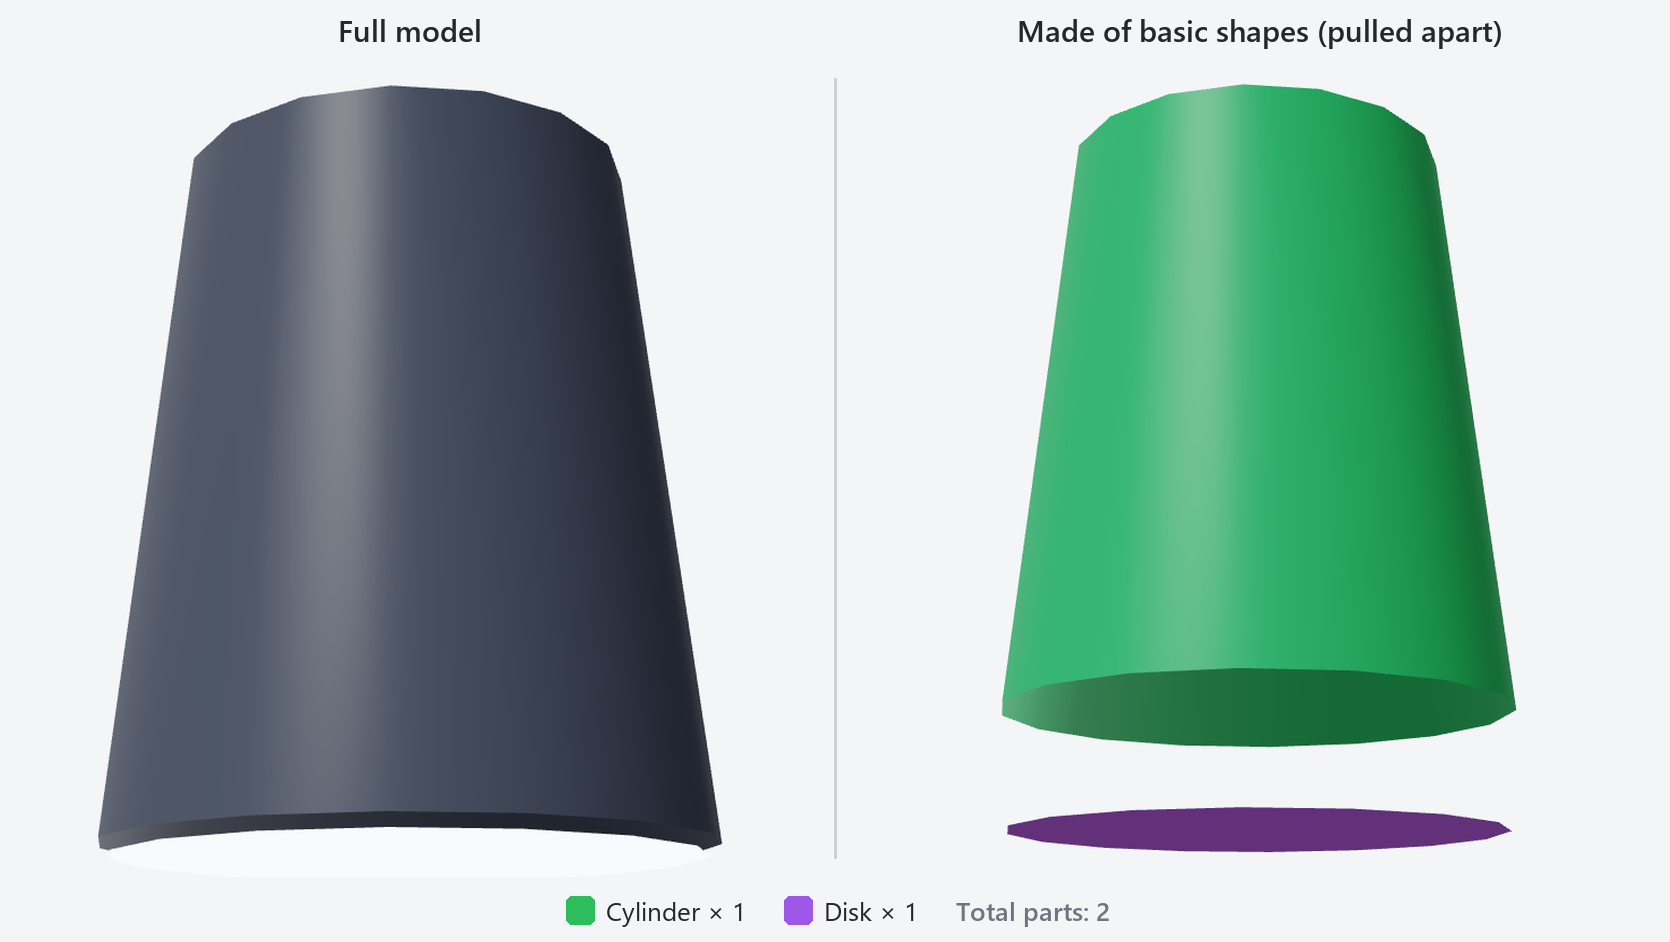
\includegraphics[width=\linewidth]{figures/decomp_spotlight.png}
\caption{Spotlight (spot)}\end{subfigure}\\[2pt]
\begin{subfigure}{0.34\linewidth}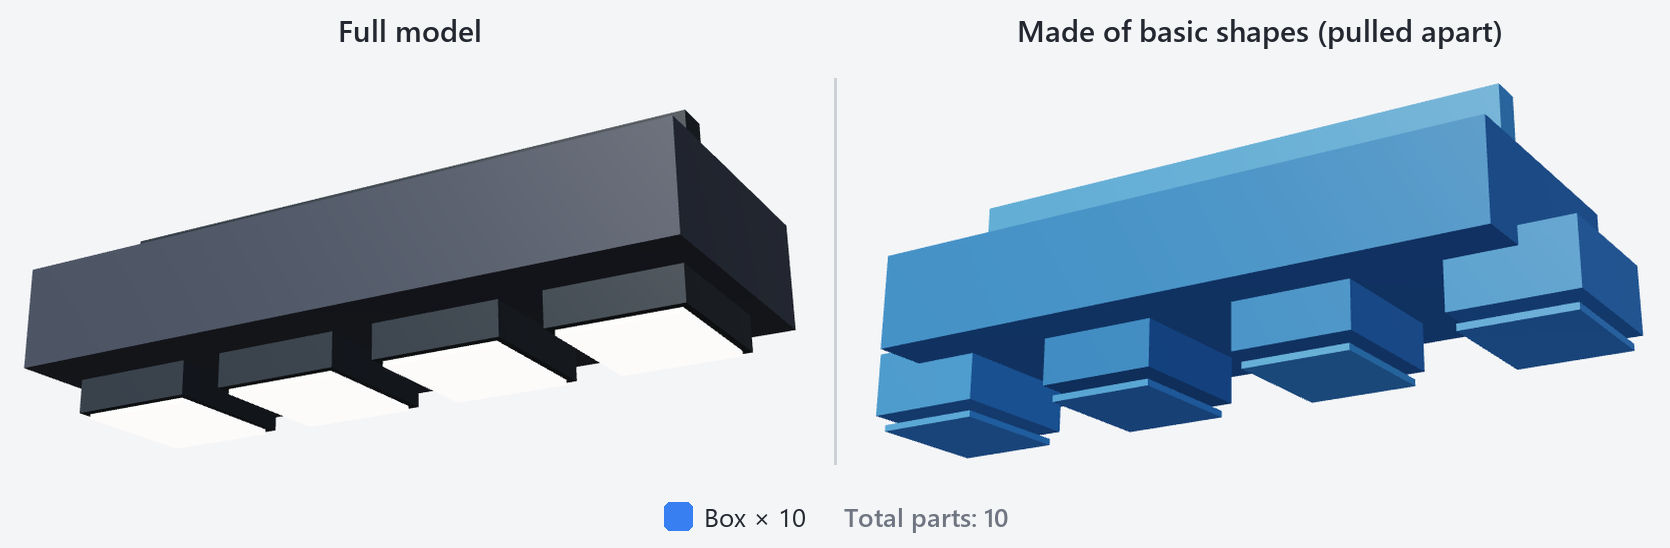
\includegraphics[width=\linewidth]{figures/decomp_gantry.png}
\caption{Gantry (directional)}\end{subfigure}\qquad
\begin{subfigure}{0.34\linewidth}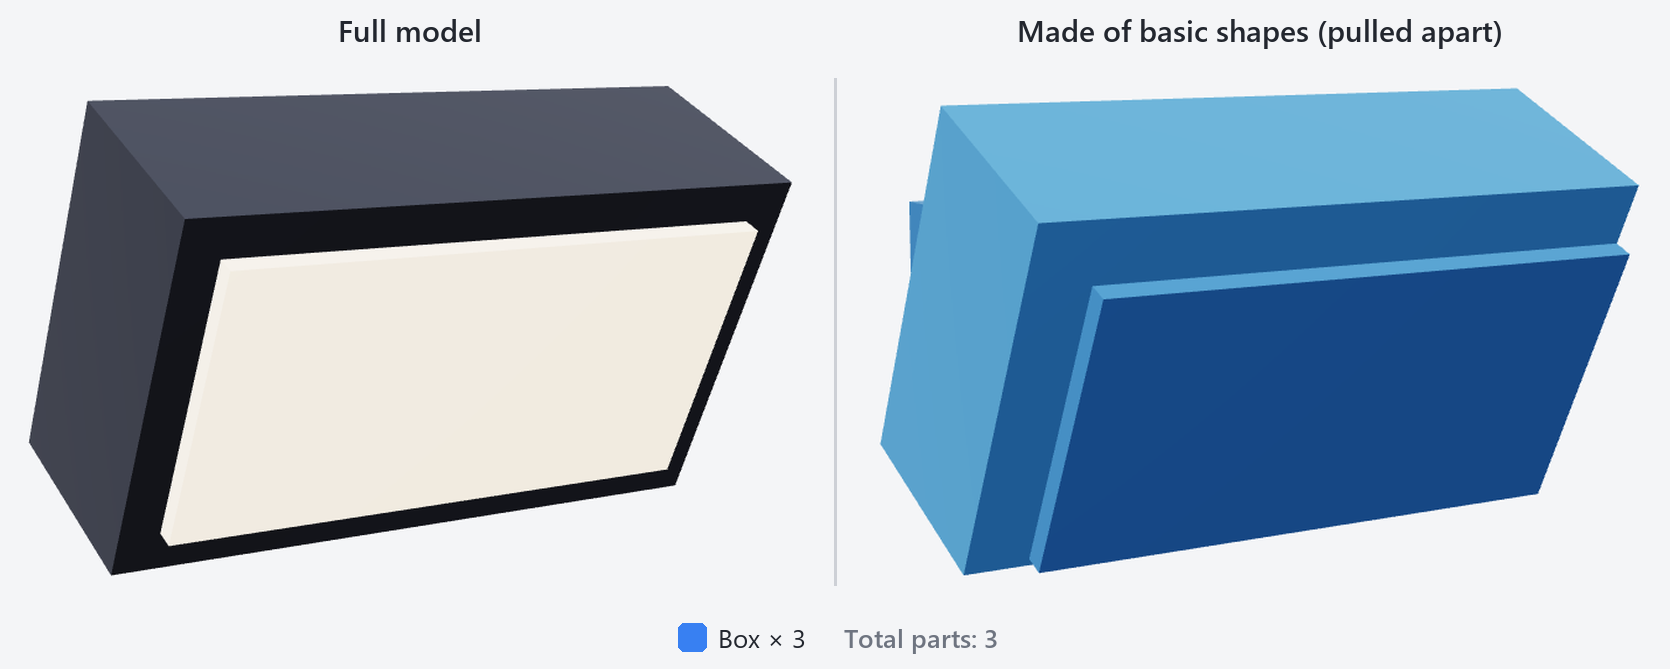
\includegraphics[width=\linewidth]{figures/decomp_walllamp.png}
\caption{Wall lamp (point)}\end{subfigure}
\caption{The light fixtures and their primitive shape composition.}
\end{figure}

\begin{table}[H]
\centering\footnotesize
\rowcolors{2}{white}{rowgray}
\begin{tabularx}{\linewidth}{p{2.6cm} L L}
\toprule
\rowcolor{white}\textbf{Fixture} & \textbf{Parts (shape, size, translate, rotate)} & \textbf{Placed at} \\ \midrule
Floodlight tower & \shBox{} pole $0.45\times16\times0.45$ at $(0,8,0)$; \shBox{} bar $2.4\times0.25\times0.6$ at $(0,16,0)$; \shBox{} housing $2.0\times0.6\times0.5$ at $(0,15.8,0)$; glowing \shBox{} lamp $1.8\times0.45\times0.08$ at $(0,15.75,-0.26)$ & $T(18,0,15)$ \\
Sun & glowing \shSph{} $r\,3.2$ + 2 faint \shSph{} halos $r\,6.0$, $10.5$ & $55\cdot(\cos e\sin a,\ \sin e,\ \cos e\cos a)$, $e{=}38^\circ$, $a{=}45^\circ$ \\
Chandelier & 4 \shBox{} cables $0.06\times5.5\times0.06$ at $(1.5\cos90^\circ k,\ 2.75,\ 1.5\sin90^\circ k)$; 2 \shTor{} rings (ring $2.2$ and $1.3$); 8 \shSph{} bulbs $r\,0.25$ at $(2.2\cos45^\circ i,\ -0.22,\ 2.2\sin45^\circ i)$; glowing \shSph{} core $r\,0.95$ & $T(0,23,28)$ \\
Follow spotlight & \shCyl{} body $r\,0.40\to0.52$, height $1.2$, $R_x90^\circ$ (points down); glowing \shDsk{} lens $r\,0.5$ at $(0,-1.22,0)$ & 8.5 above the jumper \\
Ceiling gantry & \shBox{} rack $8.0\times1.2\times3.2$; \shBox{} hanger $7.2\times0.8\times0.4$ at $(0,0.95,0)$; 4 \shBox{} projectors $1.5\times0.8\times1.8$ at $(-3+2i,\ -0.6,\ 0)$, each with a glowing \shBox{} lens $1.35\times0.08\times1.6$ & ceiling, $y{=}28.2$ \\
Wall lamp $\times4$ & \shBox{} bracket $0.25\times0.25\times1.5$ at $(0,0,-0.75)$; \shBox{} housing $1.6\times0.9\times0.5$, $R_x25^\circ$; glowing \shBox{} face $1.4\times0.7\times0.05$ & $(\pm18.4,\ 23.5,\ 14\text{ or }42)$, $R_y\mp90^\circ$ \\
\bottomrule
\end{tabularx}
\caption{Light fixture parts.}
\end{table}

% -------------------------------------------------------------------------------------
\clearpage
\subsection{Round 1 arena environment}
% -------------------------------------------------------------------------------------
\begin{figure}[H]
\centering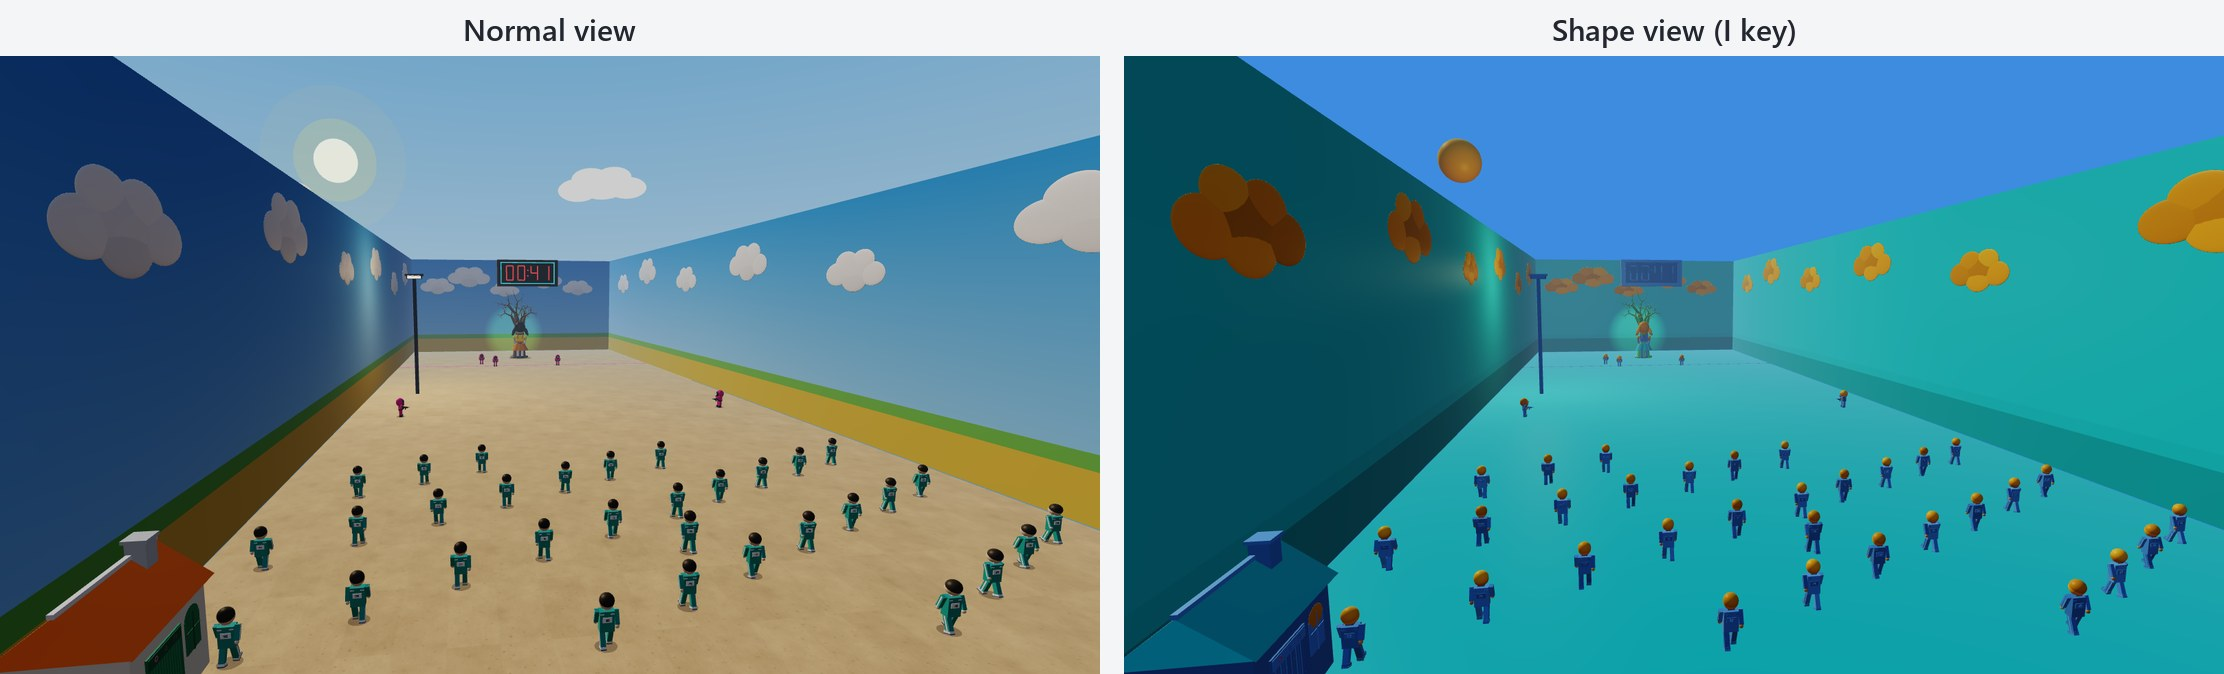
\includegraphics[width=0.92\linewidth]{figures/decomp_arena.jpg}
\caption{Round 1 arena, normal and exploded shape view. Sky dome and sand floor are polygons; clouds are clusters of spheres.}
\end{figure}

\begin{parttable}
Sky dome (new) & \shPol{} $32\times10$ quads & radius 190, pale horizon $\to$ deep blue top & centre $(0,0,0)$ & -- \\
Sky clouds (new) $\times8$ & 5 \shSph{} each & squashed spheres, radius 6.5--9 & 150 away, 34--54 high & turned to face the arena \\
Sand floor & \shPol{} $24\times32$ quads (textured) & $48\times150$, texture repeats every 6 units & $y=-0.05$ & -- \\
Painted sky walls $\times4$ & \shPol{} (quad) & $48$ or $150$ long, $22$ high, blue gradient & $x=\pm24$, $z=\pm75$ & -- \\
Wall clouds $\times23$ & 6 \shSph{} each & $S(r,\ 0.65r,\ 0.08)$, $r=1.7$--$2.5$ & on the walls & -- \\
Wheat and tree bands & \shPol{} $\times8$ & $y=0$--$3.2$ and $3.2$--$4.2$ & just inside each wall & -- \\
Start line & \shBox & $48\times0.01\times0.35$ & $(0,\ 0.01,\ -52)$ & -- \\
Finish line & \shBox{} (glowing) & $48\times0.01\times0.45$ & $(0,\ 0.01,\ 45)$ & -- \\
\end{parttable}
\note{The arena boundary is enclosed by a hemisphere sky dome ($r=190$) with smooth gradient vertex coloring and repeating sand tiles.}

% -------------------------------------------------------------------------------------
\clearpage
\subsection{Round 2 glass bridge hall environment}
% -------------------------------------------------------------------------------------
\begin{figure}[H]
\centering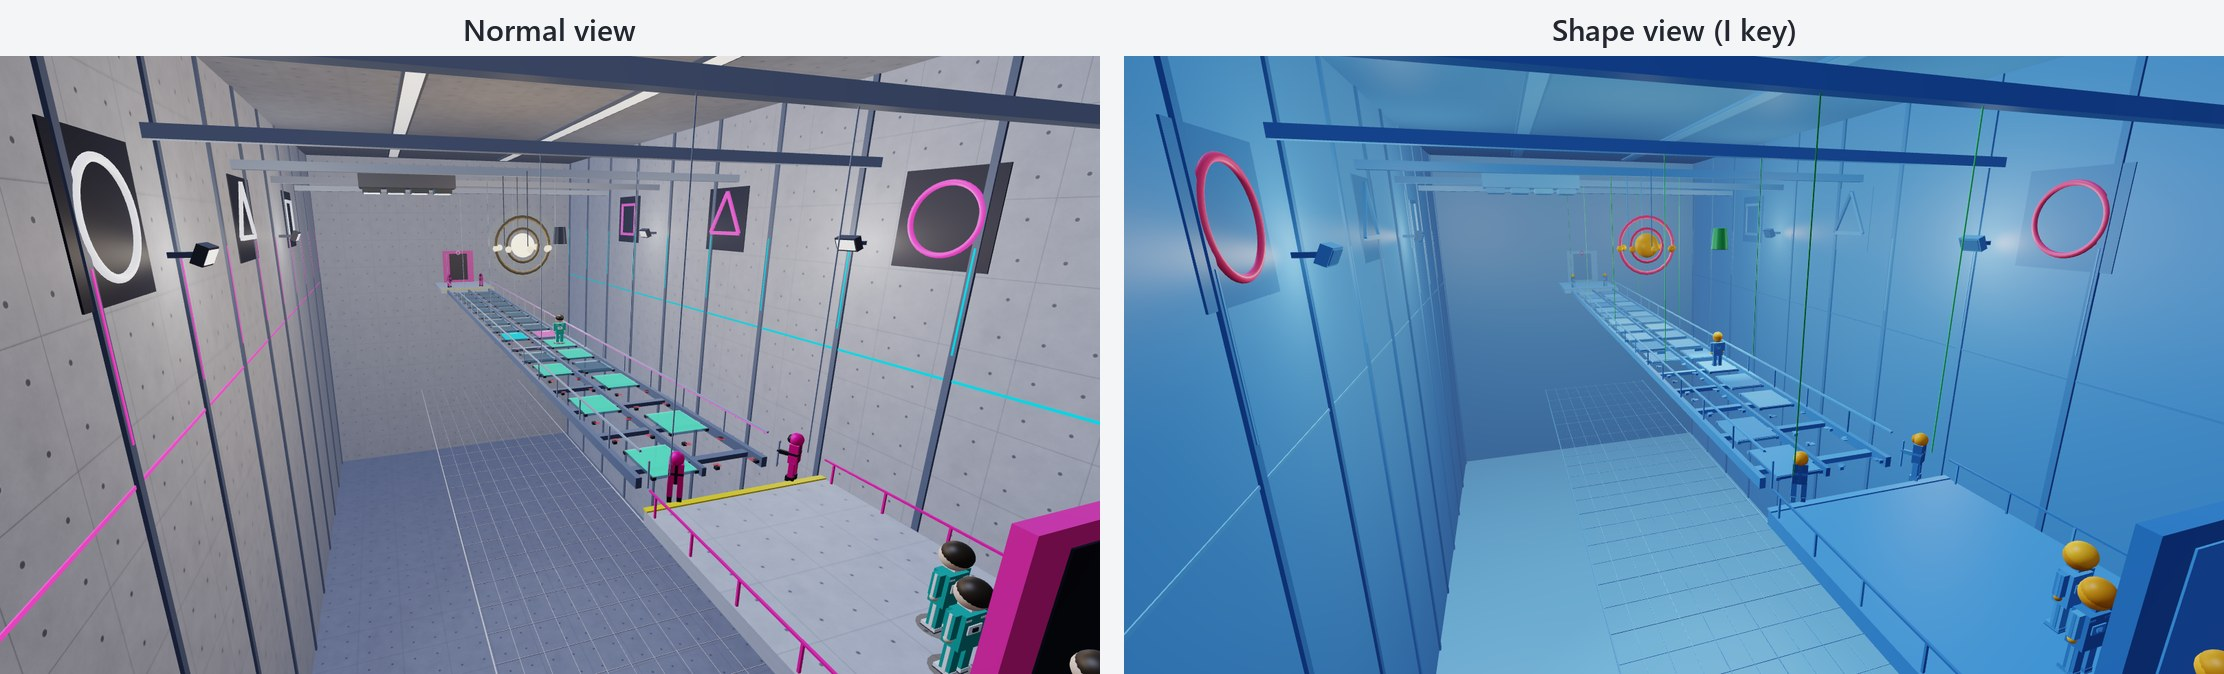
\includegraphics[width=0.92\linewidth]{figures/decomp_hall.jpg}
\caption{Round 2 hall, normal and in exploded shape view.}
\end{figure}

\begin{parttable}
Side walls $\times2$ & \shBox{} (concrete) & $0.4\times48\times88$, texture $11\times6$ times & $(\pm20,\ 10,\ 28)$ & -- \\
End walls $\times2$ & \shBox{} (concrete) & $40\times48\times0.4$ & $(0,\ 10,\ -16)$, $(0,\ 10,\ 72)$ & -- \\
Ceiling, pit floor & \shBox{} (concrete) & $40\times0.4\times88$; $40\times0.5\times88$ & $y=34$; $y=-14$ & -- \\
Ceiling light strips $\times2$ & \shBox{} $\times2$ each & $1.6\times0.25\times82$ + glowing panel & $(\pm8,\ 33.7,\ 28)$ & -- \\
Wall ribs + LED bars $\times22$ & \shBox{} $\times2$ each & $0.22\times48\times0.40$; $0.04\times6\times0.10$ & $x=\pm19.76$, $z=-9,-1,\dots,71$ & -- \\
Neon symbols $\times6$ & \shTor{} or 3/4 \shBox{} + backing \shBox & ring radius 2.0; triangle side 4.2; square side 3.6 & $(\pm19.7,\ 25,\ 9\,|\,29\,|\,49)$ & $R_y\mp90^\circ$; triangle sides $R_z\pm30^\circ$ \\
Neon wall lines $\times2$ & \shBox{} (glowing) & $0.05\times0.14\times88$ & $(\pm19.78,\ 16,\ 28)$ & -- \\
Roof trusses $\times5$ & \shBox & $40\times0.6\times0.6$ & $(0,\ 28.5,\ 0..56$ every $14)$ & -- \\
Hanging cables $\times10$ & \shCyl & radius $0.025$, length $11.4$ & $(\pm2.75,\ 17.1,\ \text{truss } z)$ & $R_x{-90}^\circ$ \\
Safety net & \shBox{} $\times39$ & cables $0.03$ thick & $y=2$, $14\times60$ area & -- \\
\end{parttable}
\note{The hall features 22 pairs of LED wall ribs, structural roof trusses, hanging suspension cables, and an emergency safety net spanning $14\times60$ units.}

% =====================================================================================
\clearpage
\section{Lighting}\label{sec:lighting}
% =====================================================================================
The game uses all three classic light types. The shader adds up the light from every lamp for every pixel.

\begin{table}[H]
\centering\small
\rowcolors{2}{white}{rowgray}
\begin{tabularx}{\linewidth}{p{2.4cm} L L L}
\toprule
\rowcolor{white}\textbf{Light type} & \textbf{Idea} & \textbf{Round 1} & \textbf{Round 2} \\ \midrule
Directional & Far away like the sun. Same direction everywhere, no fading. & The sun (elevation $38^\circ$, azimuth $45^\circ$) & Ceiling gantry (elevation $50^\circ$) \\
Point & Shines in all directions from one spot. Gets weaker with distance. & Floodlight tower at $(18,16,15)$ & Chandelier at $(0,23,28)$ \textbf{+ 4 new wall lamps} \\
Spot & A point light limited to a cone, with a soft edge. & From the doll's eyes: red when she looks, green when she sings & Follows the jumping player from above \\
\bottomrule
\end{tabularx}
\caption{The three light types in each round. Keys \keybox{0}, \keybox{8}, \keybox{9} turn them on and off.}
\end{table}

\textbf{How strong is the light at a point?}

\begin{itemize}
  \item \textbf{Diffuse} (matte brightness): $\;\max(N\cdot L,\ 0)$ -- brightest when the surface faces the light.
  \item \textbf{Specular} (shiny spot, Blinn-Phong): $\;\max(N\cdot H,\ 0)^{n}$, where $H=\dfrac{L+V}{|L+V|}$ and
        $n$ is the shininess (bigger $n$ = smaller, sharper highlight).
  \item \textbf{Point light fading:} $\;f(d)=\dfrac{I}{1+k_l\,d+k_q\,d^2}$ \quad
        (tower: $I{=}1.15,\ k_l{=}0.035,\ k_q{=}0.005$; wall lamps: $I{=}1.25,\ k_l{=}0.030,\ k_q{=}0.004$).
  \item \textbf{Spot cone:} $\;\text{cone}=\operatorname{clamp}\!\left(\dfrac{\cos\theta-\cos23^\circ}{\cos15^\circ-\cos23^\circ},\,0,\,1\right)$.
        Inside $15^\circ$ the light is full, outside $23^\circ$ it is zero, in between it fades.
\end{itemize}

\begin{lstlisting}
// GLSL Point Light computation with quadratic distance attenuation
vec3 calcPointLight(PointLight light, vec3 normal, vec3 fragPos, vec3 viewDir) {
    vec3 lightDir = normalize(light.position - fragPos);
    float diff = max(dot(normal, lightDir), 0.0);
    vec3 halfwayDir = normalize(lightDir + viewDir);
    float spec = pow(max(dot(normal, halfwayDir), 0.0), shininess);
    float dist = length(light.position - fragPos);
    float atten = 1.0 / (light.constant + light.linear * dist + light.quadratic * dist * dist);
    return (light.ambient + diff * light.diffuse + spec * light.specular) * atten;
}
\end{lstlisting}

\begin{figure}[H]
\centering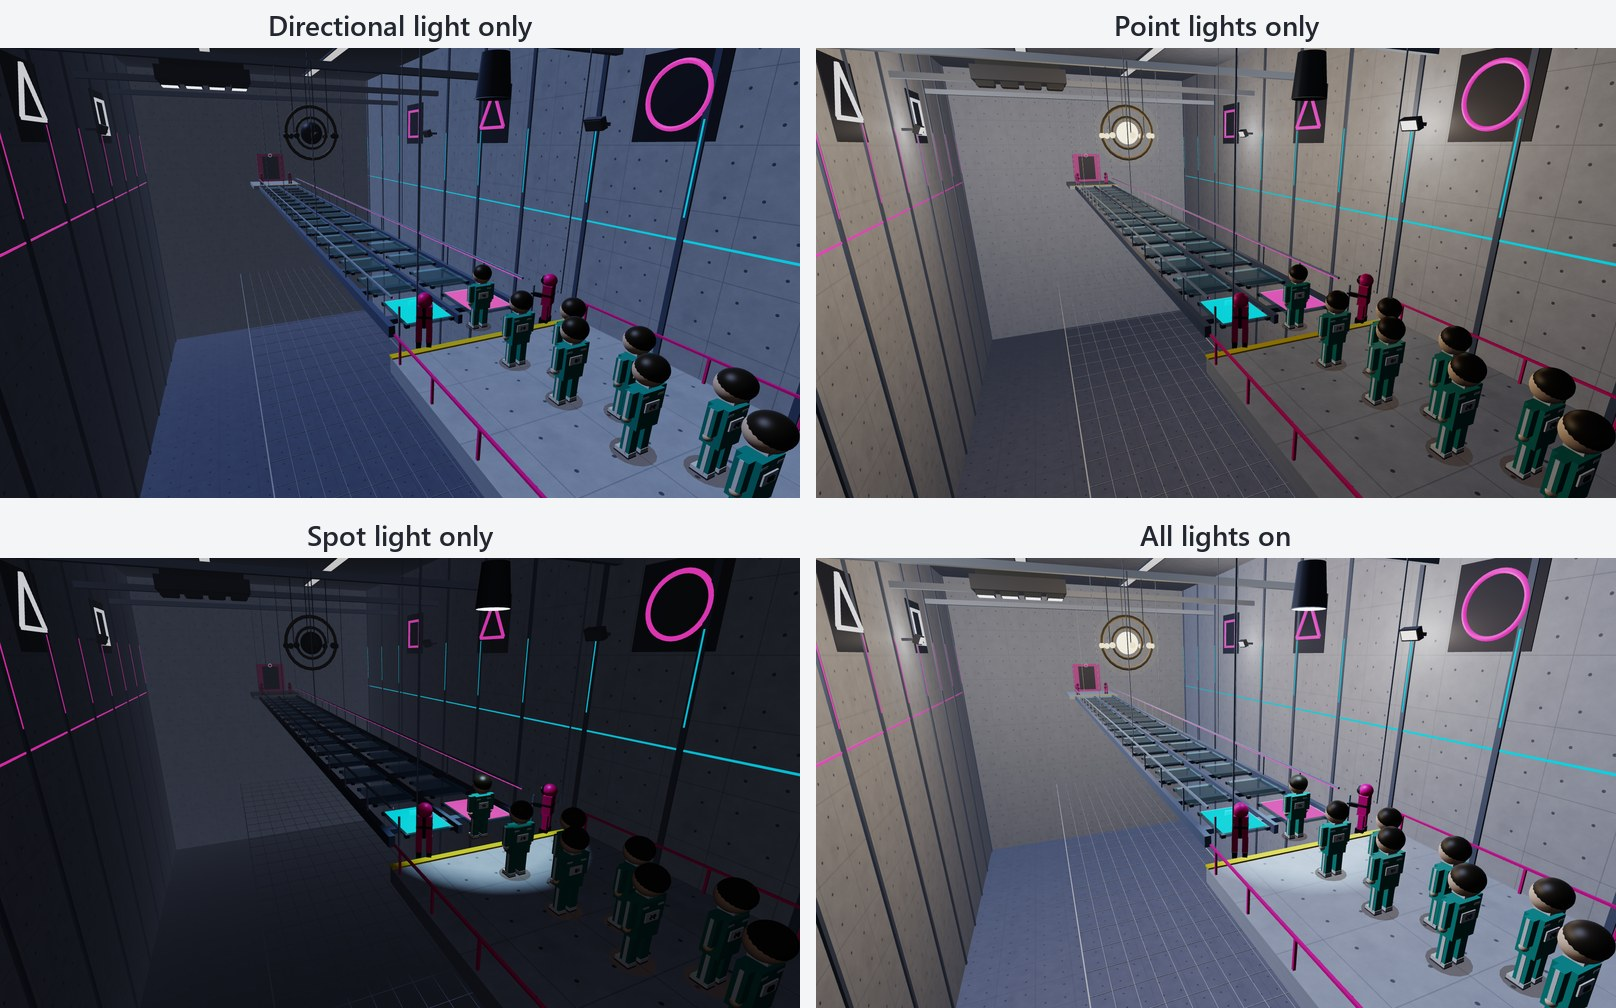
\includegraphics[width=\linewidth]{figures/lights_gb.jpg}
\caption{Round 2. Directional: even light from above. Point: warm light around the chandelier and the
wall lamps. Spot: a bright circle on the player waiting at the front.}
\end{figure}

\begin{figure}[H]
\centering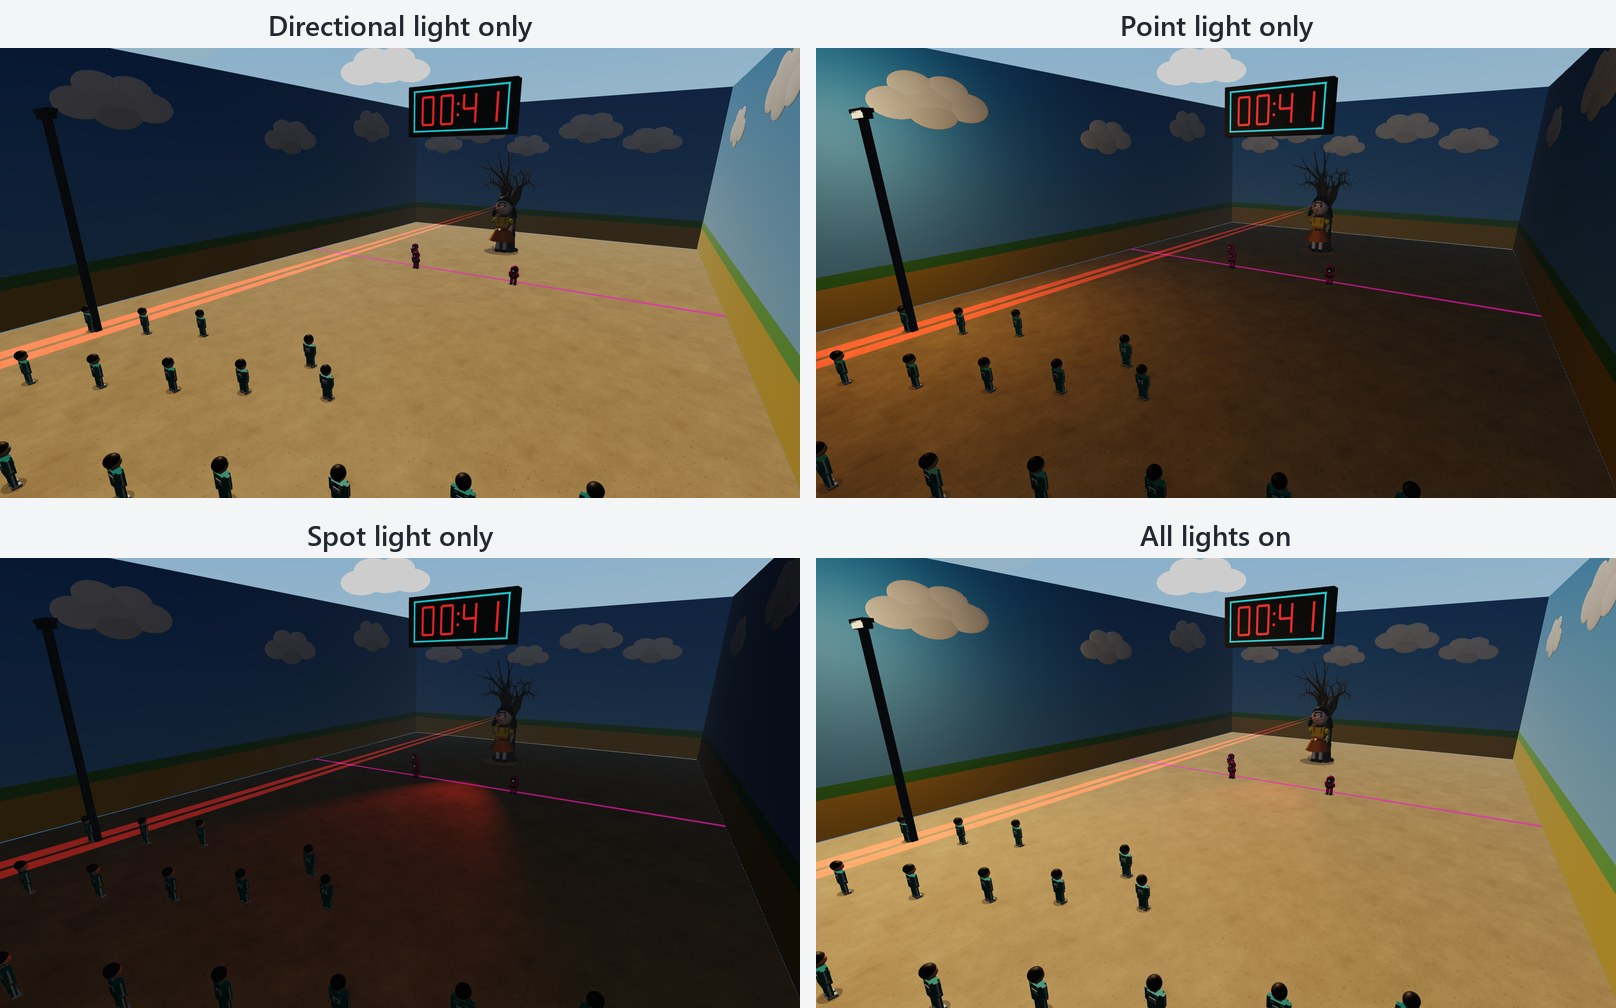
\includegraphics[width=\linewidth]{figures/lights_rlgl.jpg}
\caption{Round 1 (red light). Directional: sunlight on everything. Point: warm glow near the tower.
Spot: a red cone from the doll's eyes lights the sand in front of her.}
\end{figure}

\needspace{6\baselineskip}
\textbf{Extra light effects.}
\begin{itemize}
  \item \textbf{Ambient:} a soft base light so shadows are not pitch black. It mixes a sky color (from above)
        and a ground color (from below).
  \item \textbf{Emission:} glowing parts (neon, lamp faces, the clock digits) add their own color.
  \item \textbf{Haze:} far away surfaces slowly fade into a haze color, $\text{visibility}=e^{-(0.0075\,d)^2}$
        in Round 2. This adds depth to big spaces.
\end{itemize}

% =====================================================================================
\section{Phong Shading}\label{sec:phong}
% =====================================================================================
\textbf{Shading} decides the color of each pixel inside a triangle. This project uses \textbf{Phong shading}:
the light is calculated \emph{separately for every pixel}.

\begin{enumerate}
  \item The \textbf{vertex shader} only moves each corner (vertex) into place and passes its normal on.
  \item The GPU \textbf{interpolates} (blends) the normals across the triangle.
  \item The \textbf{fragment shader} \textbf{re-normalizes} the normal for each pixel and computes
        ambient + diffuse + specular for every light.
\end{enumerate}

\[
\text{color} = \underbrace{k_a\,C_{\text{ambient}}}_{\text{ambient}}
+ \sum_{\text{lights}}\Big(\underbrace{\max(N\!\cdot\!L,0)\,C_{\text{light}}}_{\text{diffuse}}\,\text{base}
+ \underbrace{k_s\max(N\!\cdot\!H,0)^{n}\,C_{\text{light}}}_{\text{specular}}\Big) + \text{emission}
\]

Because the normal is correct at every pixel, curved things look smooth and get small, sharp highlights
even in the middle of a triangle -- see the doll's eyes and lips and the players' heads.

\begin{figure}[H]
\centering
\begin{subfigure}{0.495\linewidth}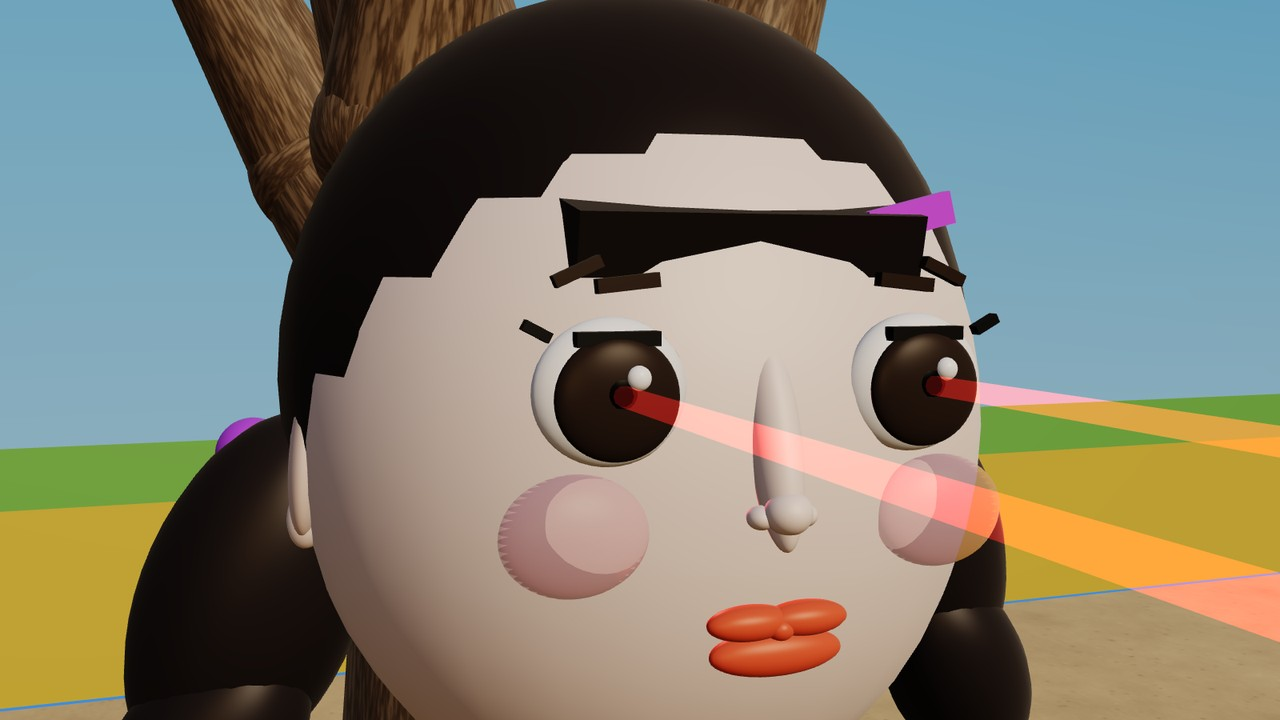
\includegraphics[width=\linewidth]{figures/phong_doll.jpg}
\caption{Shiny highlights on the doll's eyes, lips and hair.}\end{subfigure}\hfill
\begin{subfigure}{0.495\linewidth}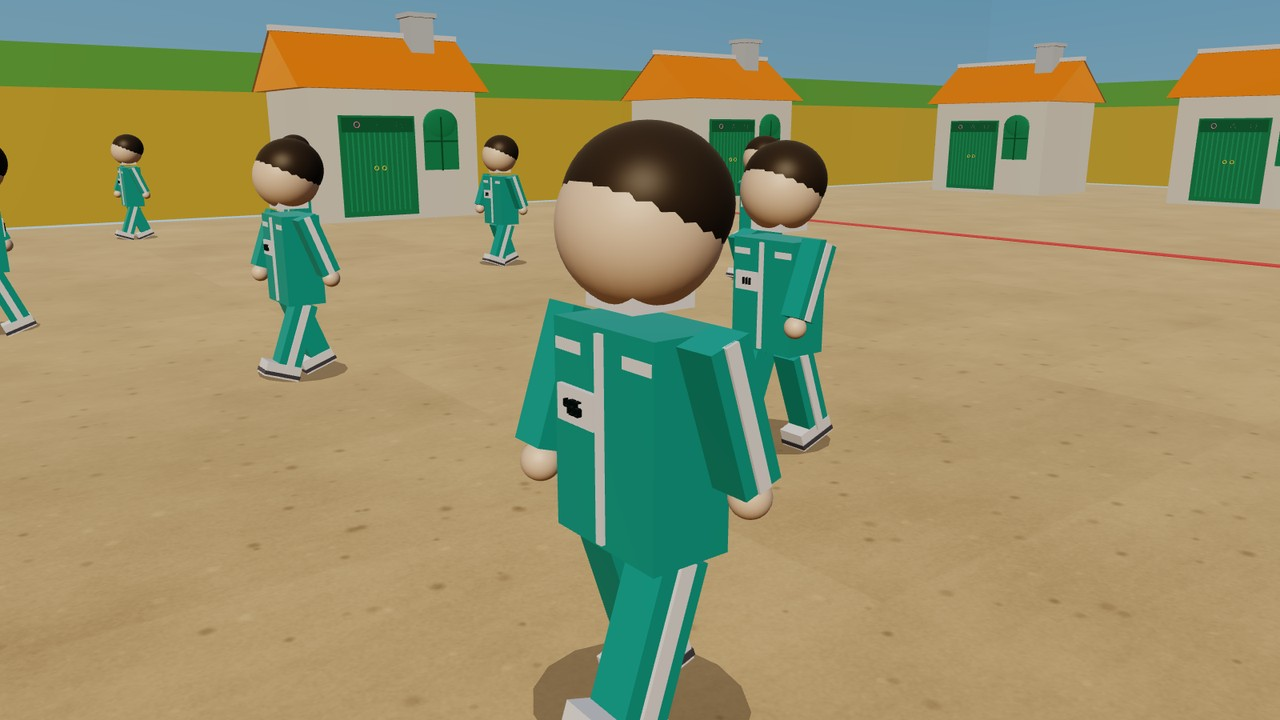
\includegraphics[width=\linewidth]{figures/phong_players.jpg}
\caption{Smooth light and highlights on round heads.}\end{subfigure}
\caption{Phong shading, close up.}
\end{figure}

The heart of the fragment shader (\texttt{src/shaders/default.frag}):
\begin{lstlisting}
// Blinn-Phong diffuse + specular of one light coming from direction L
void addLight(vec3 N, vec3 V, vec3 L, vec3 lightColor, float diffuseScale,
              float specScale, float specExp, inout vec3 diffuse, inout vec3 specular) {
    float diff = max(dot(N, L), 0.0);                 // Lambert: cos(angle to light)
    diffuse += diff * lightColor * diffuseScale;
    vec3 H = normalize(L + V);                        // halfway vector
    float spec = pow(max(dot(N, H), 0.0), specExp);   // shininess = highlight size
    specular += spec * lightColor * specScale * materialSpecularStrength;
}
...
vec3 N = normalize(Normal);                // per-pixel normal: this is Phong shading
vec3 V = normalize(viewPos - FragPos);     // direction to the camera
\end{lstlisting}

% =====================================================================================
\section{Texture Mapping}\label{sec:textures}
% =====================================================================================
A \textbf{texture} is an image wrapped onto a surface. This version adds three textures (on purpose, not
too many). They were made by a small script (\texttt{tools/make\_textures.py}) so they tile without seams.

\begin{figure}[H]
\centering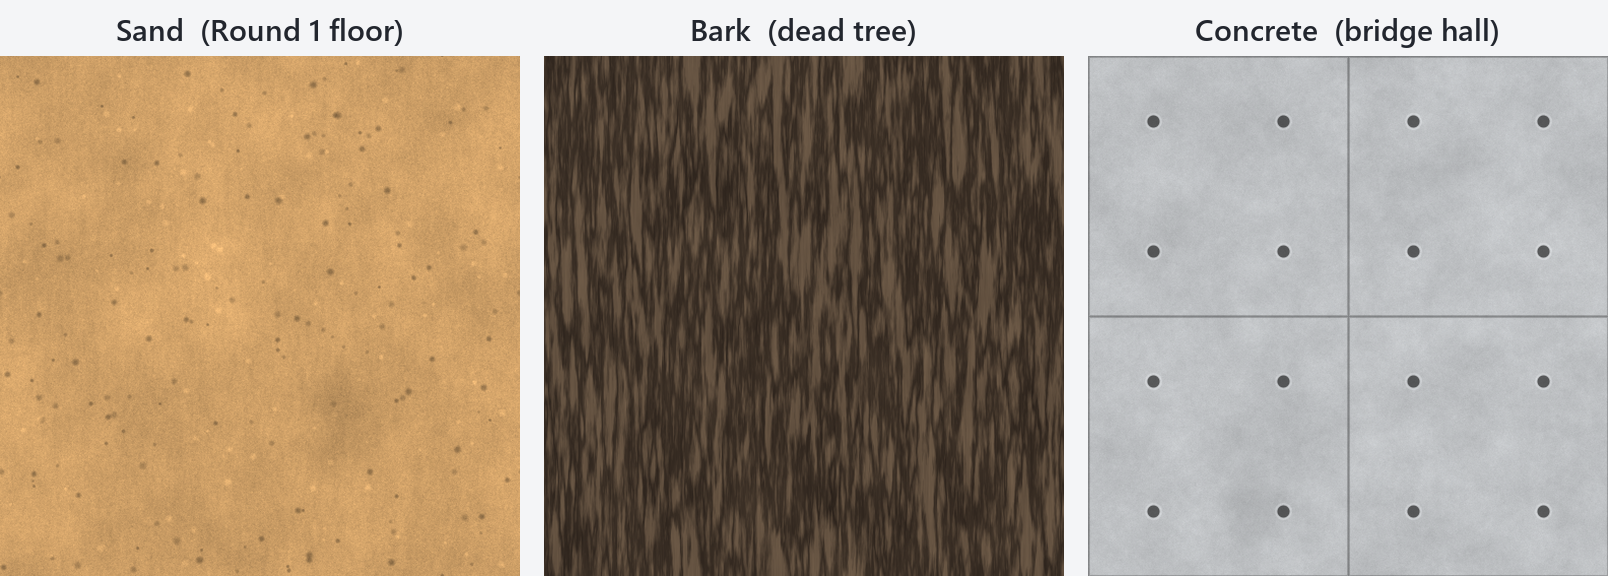
\includegraphics[width=0.92\linewidth]{figures/textures.png}
\caption{The three texture images ($512\times512$ PNG).}
\end{figure}

\textbf{How it works.}
\begin{enumerate}
  \item Each vertex now has a \textbf{texture coordinate} $(u,v)$ between 0 and 1 that says which point of the
        image belongs to it. Boxes get a $(0,0)$--$(1,1)$ square on each face, cylinders wrap $u$ around and run
        $v$ along the length, spheres use longitude/latitude.
  \item The image is loaded with \texttt{stb\_image} and uploaded once as an OpenGL texture with mipmaps
        and \texttt{GL\_REPEAT}.
  \item In the fragment shader: $\;\text{base} = \text{material} \times \text{texture}(u\cdot r_u,\ v\cdot r_v)$.
        The repeat counts $(r_u, r_v)$ tile the image so it keeps a real size on big surfaces.
\end{enumerate}

\begin{table}[H]
\centering\small
\rowcolors{2}{white}{rowgray}
\begin{tabularx}{\linewidth}{p{2.2cm} L L}
\toprule
\rowcolor{white}\textbf{Texture} & \textbf{Used on} & \textbf{How it repeats} \\ \midrule
Sand & Round 1 floor (48 $\times$ 150) & $u=x/6,\ v=z/6$: one image per $6\times6$ units \\
Bark & Every branch of the dead tree & around: $\approx4\times$radius times; along: length$/1.6$ times \\
Concrete & Round 2 walls, ceiling, pit floor and both platforms & one image per $8\times8$ units (e.g.\ side wall $11\times6$) \\
\bottomrule
\end{tabularx}
\end{table}

\begin{lstlisting}
GLCompat::setTexture(&SceneTextures::concrete(), 88.0f / 8.0f, 48.0f / 8.0f); // 11 x 6 repeats
GLCompat::drawBox(0.4f, 48.0f, 88.0f);                                        // side wall
GLCompat::clearTexture();
// fragment shader:
if (useTexture) baseColor *= texture(diffuseTexture, TexCoord * texRepeat).rgb;
\end{lstlisting}

\begin{figure}[H]
\centering
\begin{subfigure}{0.325\linewidth}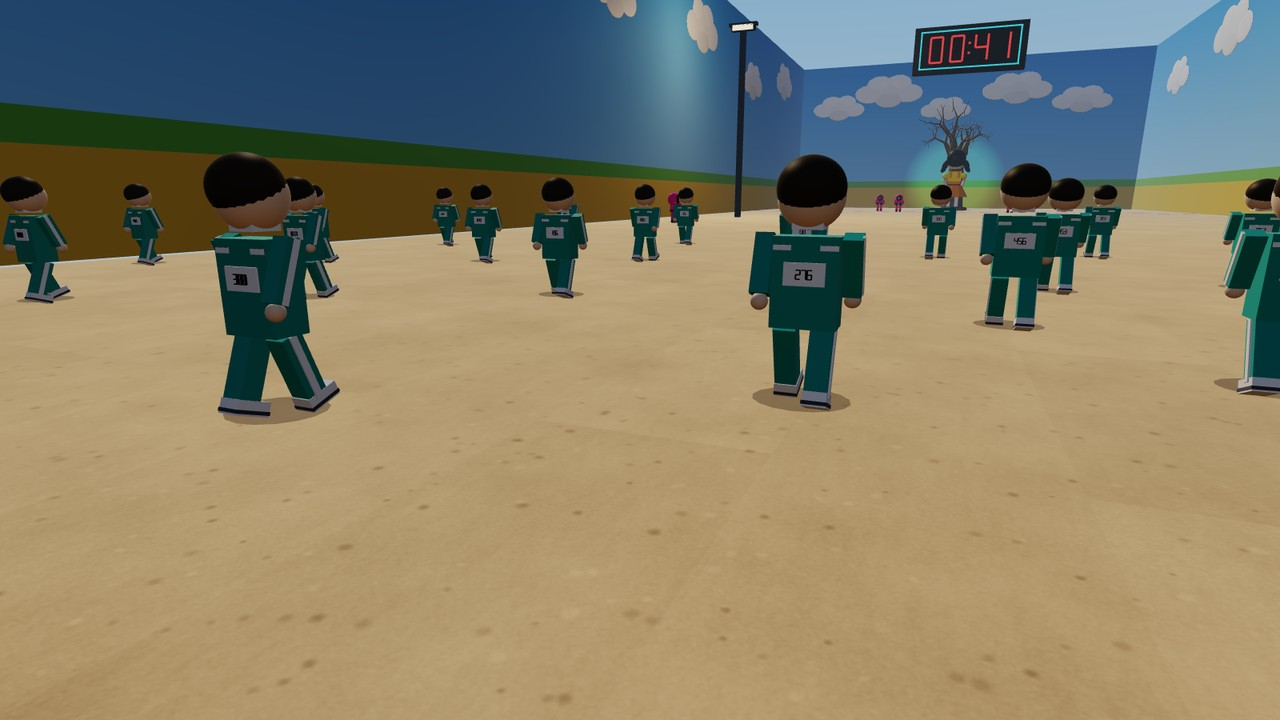
\includegraphics[width=\linewidth]{figures/tex_sand.jpg}\caption{Sand floor}\end{subfigure}\hfill
\begin{subfigure}{0.325\linewidth}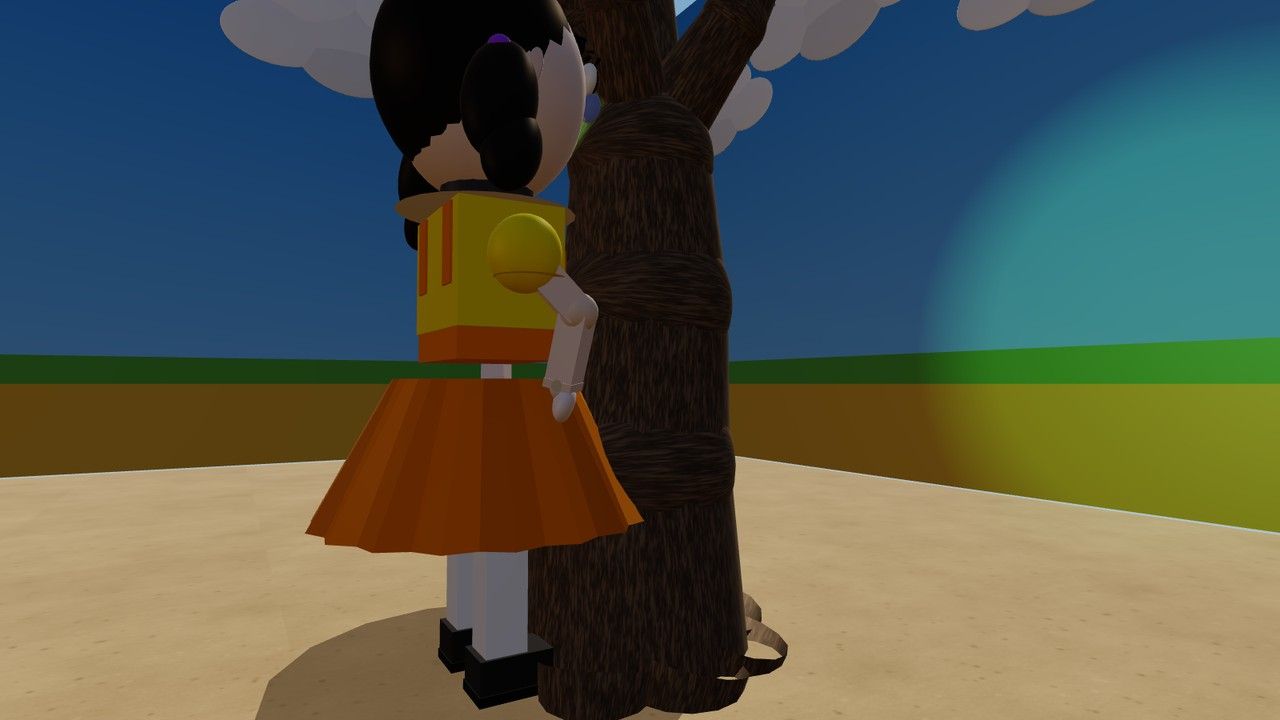
\includegraphics[width=\linewidth]{figures/tex_tree.jpg}\caption{Bark on the tree}\end{subfigure}\hfill
\begin{subfigure}{0.325\linewidth}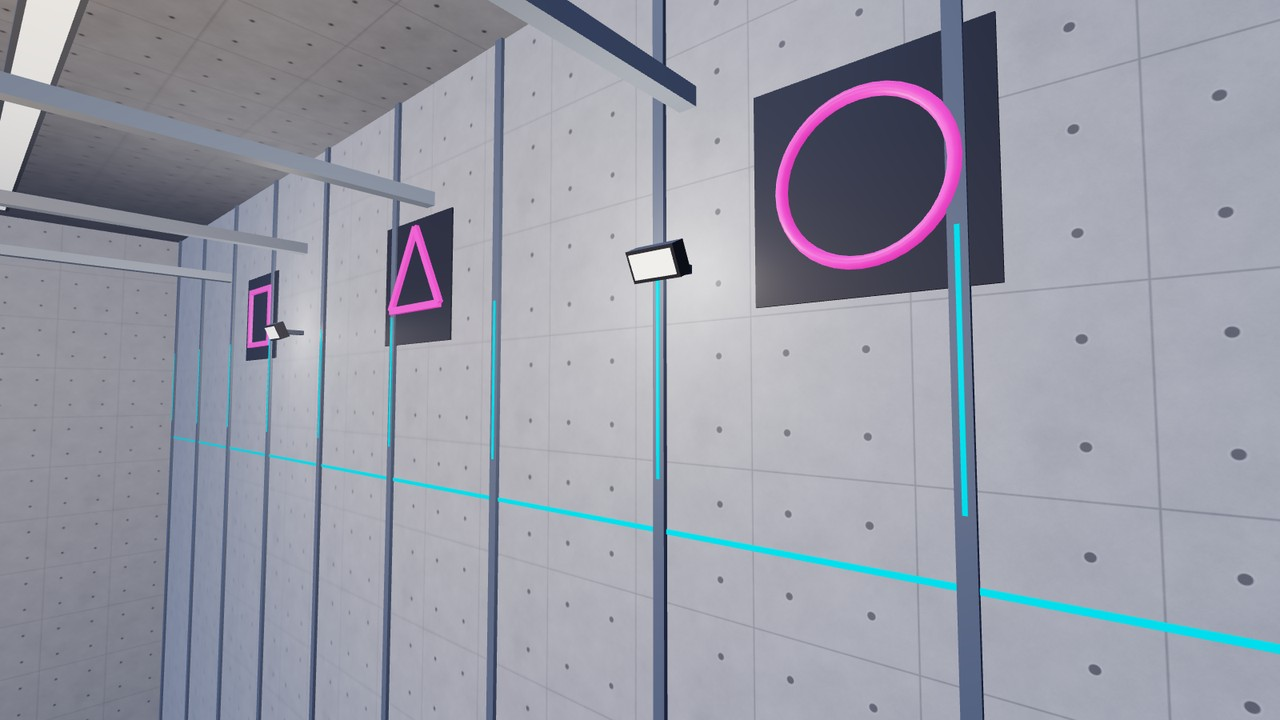
\includegraphics[width=\linewidth]{figures/tex_wall.jpg}\caption{Concrete hall wall}\end{subfigure}
\caption{The textures inside the game.}
\end{figure}

% =====================================================================================
\section{Animation and Game Logic}\label{sec:anim}
% =====================================================================================
\begin{table}[H]
\centering\small
\rowcolors{2}{white}{rowgray}
\begin{tabularx}{\linewidth}{p{3.2cm} L >{\raggedright\arraybackslash}p{5.2cm}}
\toprule
\rowcolor{white}\textbf{What moves} & \textbf{How} & \textbf{Formula} \\ \midrule
Walking legs and arms & Legs swing forward and back like a pendulum; arms swing the other way. & $\theta_{\text{leg}} = 28^\circ\sin(10\,t)$,\ $\theta_{\text{arm}}=-\theta_{\text{leg}}$ \\
Doll's head & Turns smoothly to the target angle ($0^\circ$ = singing, $180^\circ$ = looking). & $\text{angle} \mathrel{+}= (\text{target}-\text{angle})\cdot15\,\Delta t$ \\
Glass bridge jump & Moves straight to the next pane and rises in an arc. & $y = 16 + 1.3\sin(\pi p)$,\ $p: 0\to1$ in $0.42$\,s \\
Falling player & Speed grows every frame (gravity). & $v \mathrel{+}= 32\,\Delta t$,\ $y \mathrel{-}= v\,\Delta t$ \\
Glass shards (55) & Random start speed and spin, then gravity. & $v_y \mathrel{-}= 28\,\Delta t$;\ $\vec p \mathrel{+}= \vec v\,\Delta t$ \\
Blood drops (30) & Burst outward, fall, fade out. & $v_y \mathrel{-}= 9.8\,\Delta t$;\ alpha $=1-\text{life}/\text{max}$ \\
\bottomrule
\end{tabularx}
\end{table}

\textbf{Round 1 rules.}
\begin{itemize}
  \item 60 seconds to reach the finish line ($z=45$).
  \item Green light: the doll sings for 4.8--6.2 seconds. Red light: she looks for 3.2--5.2 seconds.
  \item If Player 456 moves while her head is turned past $80^\circ$, a guard shoots and the game is over.
  \item Each red light, every other contestant has an 18\% chance to be caught.
\end{itemize}

\textbf{Round 2 rules.}
\begin{itemize}
  \item 16 players take turns. Player 456 gets a random place in the queue.
  \item For every step, the strong side is chosen at random (50/50). Once a pane is proven, later players follow it.
  \item The other players choose randomly. Player 456 chooses with \keybox{A} / \keybox{D}. 16 minutes in total.
\end{itemize}

% =====================================================================================
\section{Cameras and Viewport Pipeline}\label{sec:cameras}
% =====================================================================================
The project implements a modern dual-layer camera system combining the core engine
\texttt{Camera} class in \texttt{src/engine/Camera.cpp} and the high-level game director
\texttt{CameraManager} in \texttt{src/camera/Camera.cpp}. It supports 7 real-time cinematic perspectives,
interactive 360$^\circ$ mouse orbiting, dynamic scroll zoom, exponential smoothing, and multi-pass
Picture-in-Picture (PiP) rendering.

\subsection{Camera Architecture and Mathematical Mechanism}
The camera pipeline converts 3D world-space coordinates into 2D screen coordinates using the standard
Model-View-Projection (MVP) matrix transformation:
\begin{equation}
\vec{v}_{\text{clip}} = P \cdot V \cdot M \cdot \vec{v}_{\text{local}}
\end{equation}

\textbf{1. View Matrix ($V$):} Derived from an eye position $\vec{P}_{\text{eye}}$, a look-at target
$\vec{P}_{\text{target}}$, and a world up vector $\vec{U} = (0, 1, 0)$ via \texttt{glm::lookAt}:
\begin{equation}
\vec{F} = \frac{\vec{P}_{\text{target}} - \vec{P}_{\text{eye}}}{\|\vec{P}_{\text{target}} - \vec{P}_{\text{eye}}\|}, \quad
\vec{R} = \frac{\vec{F} \times \vec{U}}{\|\vec{F} \times \vec{U}\|}, \quad
\vec{U}' = \vec{R} \times \vec{F}
\end{equation}
\begin{equation}
V = \begin{bmatrix}
R_x & R_y & R_z & -\vec{R} \cdot \vec{P}_{\text{eye}} \\
U'_x & U'_y & U'_z & -\vec{U}' \cdot \vec{P}_{\text{eye}} \\
-F_x & -F_y & -F_z & \vec{F} \cdot \vec{P}_{\text{eye}} \\
0 & 0 & 0 & 1
\end{bmatrix}
\end{equation}

\textbf{2. Perspective Projection Matrix ($P$):} Defined by the vertical field of view ($\text{fov}_y$),
viewport aspect ratio ($\text{aspect} = W/H$), near clipping plane ($z_n = 0.1$), and far clipping
plane ($z_f = 280.0$):
\begin{equation}
P = \begin{bmatrix}
\dfrac{1}{\text{aspect} \cdot \tan(\text{fov}/2)} & 0 & 0 & 0 \\[6pt]
0 & \dfrac{1}{\tan(\text{fov}/2)} & 0 & 0 \\[6pt]
0 & 0 & -\dfrac{z_f + z_n}{z_f - z_n} & -\dfrac{2 z_f z_n}{z_f - z_n} \\[6pt]
0 & 0 & -1 & 0
\end{bmatrix}
\end{equation}

The core camera matrix update implemented in \texttt{src/engine/Camera.cpp}:
\begin{lstlisting}
void Camera::SetView(const glm::vec3& eye, const glm::vec3& target, const glm::vec3& up,
                     float fovDeg, float nearPlane, float farPlane) {
    Position    = eye;
    Orientation = glm::normalize(target - eye);
    Up          = up;
    view        = glm::lookAt(eye, target, up);
    projection  = glm::perspective(glm::radians(fovDeg),
                                   (float)width / (float)height,
                                   nearPlane, farPlane);
}
\end{lstlisting}

\subsection{Screen Dimensions, Aspect Ratio, and Viewport Calculation}
A fundamental requirement in 3D graphics is ensuring that objects retain their true geometric proportions
regardless of screen resolution or window resizing. Without continuous aspect ratio recalculation, spheres
and character heads would distort into stretched ellipsoids.

\textbf{Resolution Handling and GLFW Callbacks:}
The game defaults to a $1600 \times 900$ desktop window and scales seamlessly to Full HD $1920 \times 1080$,
$2560 \times 1440$, or user-resized dimensions. Physical framebuffer dimensions are tracked via GLFW:
\begin{lstlisting}
void framebufferSizeCallback(GLFWwindow*, int w, int h) {
    windowWidth  = (w > 0) ? w : 1;
    windowHeight = (h > 0) ? h : 1;
}
\end{lstlisting}

\textbf{Split-Screen HUD Viewport Calculation:}
The game UI features two persistent sidebar panels:
\begin{itemize}
  \item \textbf{Left Sidebar ($W_{\text{left}} = 300$\,px):} Houses the live CCTV doll camera feed, countdown timer, contestant counters, and arena mini-radar.
  \item \textbf{Right Sidebar ($W_{\text{right}} = 300$\,px):} Houses camera mode buttons, speed controls, and interactive lighting toggles.
\end{itemize}

Rather than rendering the 3D scene underneath the HUD overlays, the 3D rendering pipeline calculates
an independent center viewport:
\begin{equation}
W_{\text{center}} = W_{\text{window}} - W_{\text{left}} - W_{\text{right}}, \qquad
\text{Aspect}_{\text{3D}} = \frac{W_{\text{center}}}{H_{\text{window}}}
\end{equation}

For example, on a standard Full HD display of $1920 \times 1080$:
\begin{itemize}
  \item Total screen: $W_{\text{window}} = 1920$, $H_{\text{window}} = 1080$. Fullscreen aspect ratio: $\frac{1920}{1080} = \frac{16}{9} \approx 1.778$.
  \item Center 3D viewport: $W_{\text{center}} = 1920 - 300 - 300 = 1320$\,px.
  \item Rendered 3D aspect ratio: $\text{Aspect}_{\text{3D}} = \frac{1320}{1080} \approx 1.222$.
\end{itemize}

The viewport and projection matrices are dynamically updated every frame in \texttt{src/main\_modern.cpp}:
\begin{lstlisting}
int leftBarW = UI_LEFT_BAR_WIDTH, rightBarW = UI_RIGHT_BAR_WIDTH;
int centerW  = (drawUI && windowWidth > 600) ? (windowWidth - leftBarW - rightBarW) : windowWidth;
glViewport(drawUI ? leftBarW : 0, 0, centerW, windowHeight);
camera.width = centerW; camera.height = windowHeight;
camera.SetView(glm::vec3(eyeX, eyeY, eyeZ), glm::vec3(lookX, lookY, lookZ),
               glm::vec3(upX, upY, upZ), fov, 0.1f, 280.0f);
\end{lstlisting}
When the user toggles the HUD off (\keybox{H}), the sidebars collapse to 0, expanding $W_{\text{center}} = 1920$
and restoring the native $16:9$ ($1.778$) aspect ratio without any geometric stretching.

\subsection{Smooth Camera Easing and Interactive Orbiting}
To prevent abrupt camera snapping when switching perspectives or moving rapidly, the camera interpolates
its coordinates using exponential damping:
\begin{equation}
\vec{P}_{\text{cam}}(t + \Delta t) = \vec{P}_{\text{cam}}(t) + \big(\vec{P}_{\text{target}} - \vec{P}_{\text{cam}}(t)\big) \cdot \big(1 - e^{-k\,\Delta t}\big)
\end{equation}
where $k = 12.0$ for close-up tracking and $k = 8.0$ for wide arena perspectives.

\textbf{Mouse Orbit Controls:}
Users can freely orbit $360^\circ$ around the player or the doll by dragging the mouse. The pitch ($\theta$)
and yaw ($\phi$) spherical coordinates are translated into Cartesian eye offsets:
\begin{equation}
\Delta x = d \cos\theta \sin\phi, \quad \Delta y = d \sin\theta, \quad \Delta z = d \cos\theta \cos\phi
\end{equation}
Mouse scroll wheel deltas dynamically scale distance $d$, clamped within safety limits ($1.8 \le d \le 18.0$
for 3rd person; $2.0 \le d \le 38.0$ for the doll).

\subsection{Camera Perspectives and Multi-Pass CCTV Rendering}
The game features 7 primary camera perspectives and an independent secondary rendering pass:

\begin{table}[H]
\centering\small
\rowcolors{2}{white}{rowgray}
\begin{tabularx}{\linewidth}{c >{\bfseries}p{3.2cm} c L}
\toprule
\rowcolor{white}\textbf{Key} & \textbf{Camera Mode} & \textbf{FOV} & \textbf{Behavior and Target} \\ \midrule
\keybox{1} & 3rd Person Follow & $55^\circ$ & Follows Player 456; supports $360^\circ$ mouse orbit and arena collision clamping \\
\keybox{2} & Overhead Drone & $55^\circ$ & High stadium overview ($d=58$); full arena free-orbit and zoom \\
\keybox{3} & Top-Down Aerial & $58^\circ$ & Plan view centered at $(0, 110, -3.5)$ with north aligned forward \\
\keybox{4} & Doll $360^\circ$ Orbit & $55^\circ$ & Orbiting camera anchored at the doll's head $(0, 8.5, 58)$ \\
\keybox{5} & Left Broadcast & $55^\circ$ & Elevated broadcast perspective from the left wall $(-20.5, 12, z_{\text{player}}+5)$ \\
\keybox{6} & Right Broadcast & $55^\circ$ & Symmetrical broadcast perspective from the right wall $(+20.5, 12, z_{\text{player}}+5)$ \\
\keybox{7} & Finish Line POV & $55^\circ$ & Located at $z=45$ facing backwards to watch oncoming contestants \\
\bottomrule
\end{tabularx}
\caption{The 7 dynamic camera modes available in the game.}
\end{table}

\textbf{Multi-Pass CCTV Doll Camera:}
In addition to the main viewport, the engine executes a dedicated secondary rendering pass in Round 1:
\begin{enumerate}
  \item \textbf{Pass 1 (Main Scene):} Renders the central 3D viewport using the player's active camera mode.
  \item \textbf{Pass 2 (HUD):} Draws ImGui sidebars and panels over the window.
  \item \textbf{Pass 3 (CCTV Doll Cam):} Renders an over-the-shoulder POV ($\text{FOV} = 48^\circ$) into the left panel frame via \texttt{glViewport}.
\end{enumerate}

\begin{figure}[H]
\centering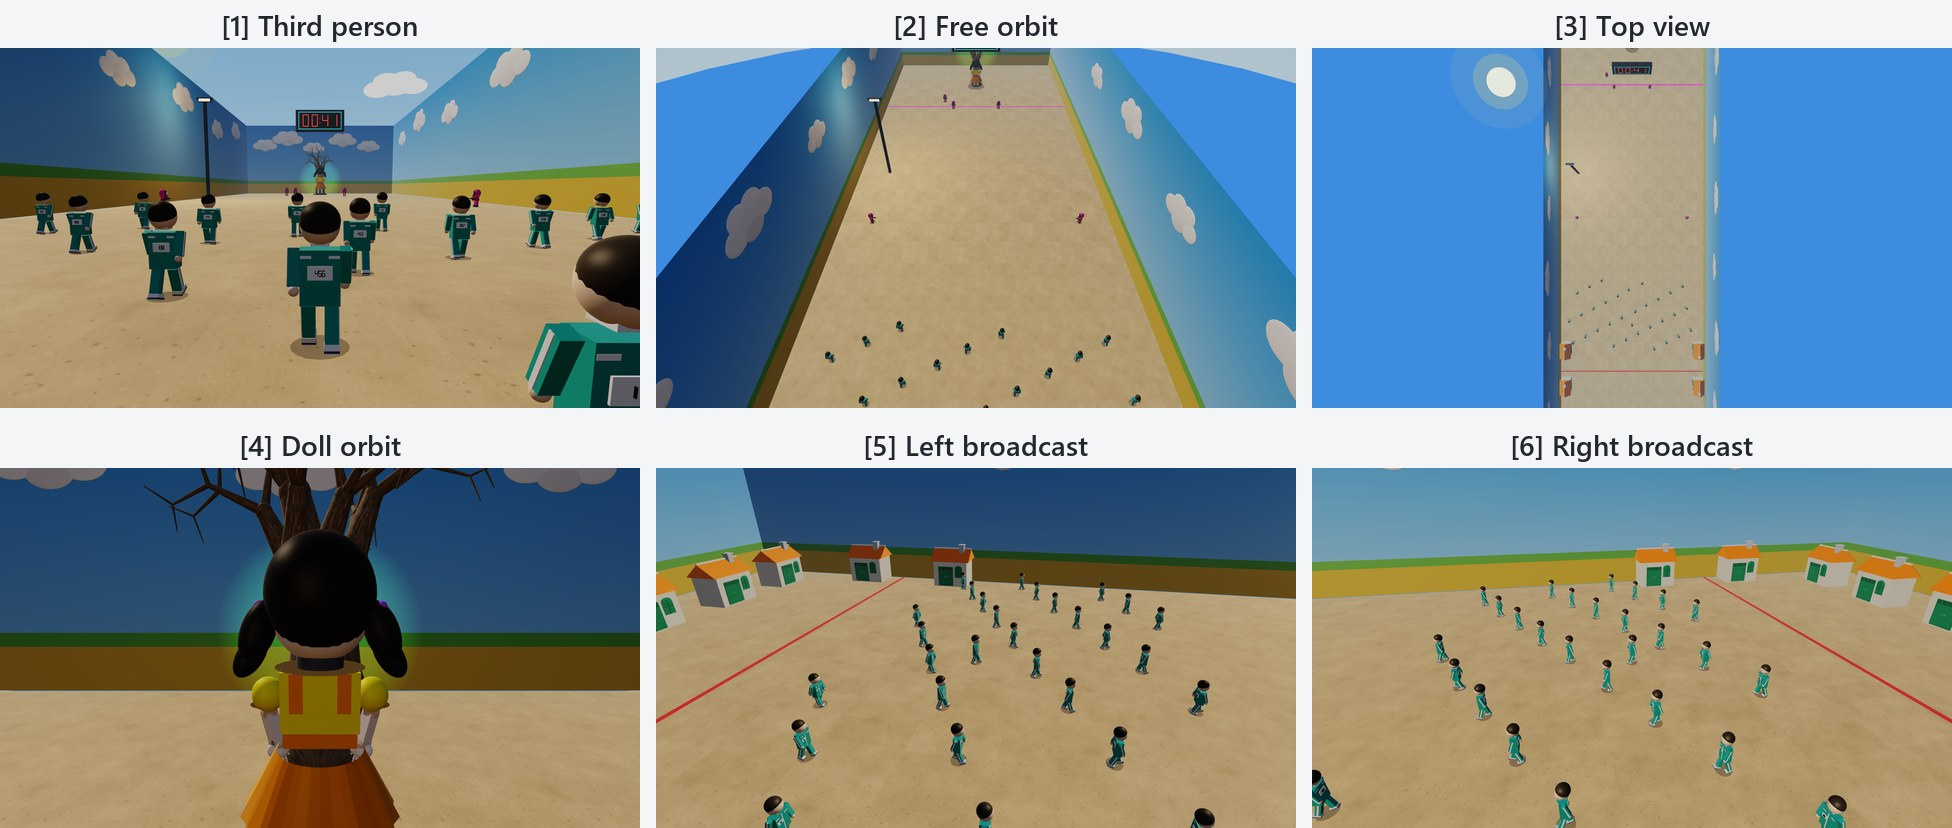
\includegraphics[width=\linewidth]{figures/cameras_rlgl.jpg}
\caption{Round 1 camera modes (keys 1--6).}
\end{figure}

\begin{figure}[H]
\centering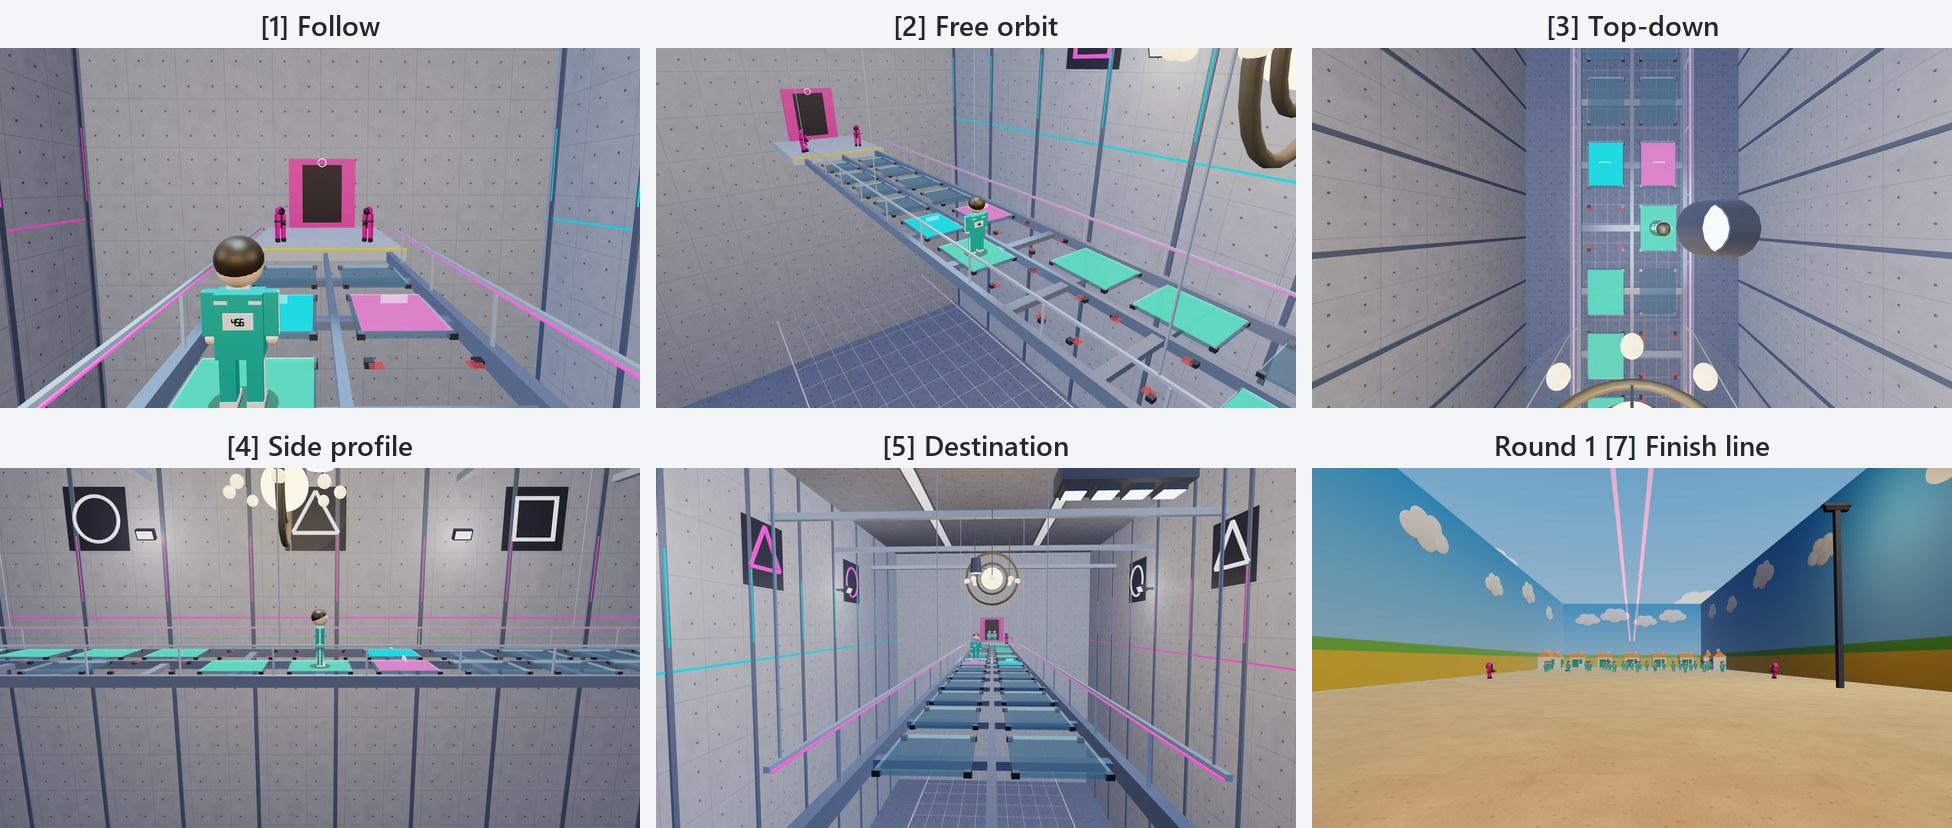
\includegraphics[width=\linewidth]{figures/cameras_gb.jpg}
\caption{Round 2 camera modes (keys 1--5) and Round 1's finish-line camera (key 7, during red light).}
\end{figure}

% =====================================================================================
\section{Conclusion}
% =====================================================================================
This project builds a complete two-round 3D game without loading a single 3D model. Seven basic shapes,
placed with translate, rotate and scale and organised in parent--child groups, make every object -- from a
contestant (53 parts) to the giant doll (147 parts) and the recursive tree (313 parts). The scenes are lit by
directional, point and spot lights, shaded per pixel with Phong shading, and three textures add surface detail.
The new capture and shape-view tools make it easy to see, check and explain how everything is built.

\end{document}
